% !TeX program = xelatex
\PassOptionsToPackage{table}{xcolor}
\documentclass[aspectratio=169,10pt]{beamer}
\usepackage[UTF8,fontset=fandol]{ctex}
\usepackage{amsmath,amssymb,booktabs,array,graphicx,tabularx,xurl}
\usepackage[most]{tcolorbox}
\definecolor{navy}{HTML}{173A55}
\definecolor{teal}{HTML}{087C87}
\definecolor{muted}{HTML}{566574}
\definecolor{line}{HTML}{AFC3D0}
\definecolor{zebra}{HTML}{EAF3F7}
\setbeamercolor{normal text}{fg=black,bg=white}
\setbeamercolor{frametitle}{fg=navy,bg=white}
\setbeamercolor{structure}{fg=teal}
\setbeamerfont{frametitle}{size=\fontsize{14.5}{18}\selectfont,series=\bfseries}
\setbeamerfont{normal text}{size=\fontsize{9.2}{11.7}\selectfont}
\setbeamersize{text margin left=7mm,text margin right=7mm}
\setbeamertemplate{navigation symbols}{}
\setbeamertemplate{frametitle}{\vspace{1.6mm}\noindent{\color{teal}\rule[-0.35mm]{1.2mm}{4.3mm}}\hspace{1.6mm}\insertframetitle\par\vspace{0.9mm}{\color{line}\hrule height .6pt}\vspace{1.2mm}}
\setbeameroption{hide notes}
\hypersetup{colorlinks=true,urlcolor=teal,pdftitle={群体智能的主动感知：30篇论文的方法、架构与实验研究报告},pdfauthor={研究汇报}}
\def\slidesource{}
\newcommand{\lead}[1]{\par\vspace{0.4mm}\noindent\hangindent=2.6mm\hangafter=1{\color{teal}\rule[-0.45mm]{0.9mm}{4.4mm}}\hspace{1.6mm}{\fontsize{10.1}{13}\selectfont\bfseries\color{navy}#1}\par\vspace{1.5mm}}
\newtcolorbox{takebox}{enhanced,colback=teal!6,colframe=teal,boxrule=0pt,leftrule=1.1pt,arc=0pt,outer arc=0pt,left=2.2mm,right=2.2mm,top=0.7mm,bottom=0.7mm,before skip=1.2mm,after skip=0.2mm}
\newcommand{\takeaway}[1]{\par\begin{takebox}\fontsize{9.1}{11.5}\selectfont\bfseries\color{navy}#1\end{takebox}}
\newcommand{\ph}[1]{{\color{teal}\rule[-0.35mm]{0.8mm}{3.1mm}}\hspace{1.1mm}\textbf{\color{navy}#1}}
\newcommand{\thd}[1]{\textcolor{white}{\bfseries #1}}
\newcolumntype{Y}[1]{>{\hsize=#1\hsize\linewidth=\hsize\raggedright\arraybackslash}X}
\newcolumntype{Z}[1]{>{\hsize=#1\hsize\linewidth=\hsize\centering\arraybackslash}X}
\newcommand{\bline}[2]{\par\ph{#1}\quad #2\par\vspace{1.5mm}}
\newcommand{\refentry}[5]{\par\textcolor{teal}{[#1]} #2. \emph{#3}. \href{#5}{arXiv:#4}.\par\vspace{1.5mm}}
\setbeamertemplate{footline}{\leavevmode\hbox{\begin{beamercolorbox}[wd=.92\paperwidth,ht=3mm,dp=1.5mm,leftskip=7mm]{normal text}\color{muted}\fontsize{6}{7}\selectfont\slidesource\end{beamercolorbox}\begin{beamercolorbox}[wd=.08\paperwidth,ht=3mm,dp=1.5mm,rightskip=4mm plus1fil]{normal text}\hfill\color{muted}\fontsize{7.5}{8}\selectfont\insertframenumber\end{beamercolorbox}}}
\setlength{\tabcolsep}{3.5pt}
\renewcommand{\arraystretch}{1.14}
\setlength{\extrarowheight}{0.35pt}
\arrayrulecolor{line}
\setlength{\heavyrulewidth}{0.85pt}
\setlength{\lightrulewidth}{0.45pt}
\setlength{\parskip}{1pt}
\setlength{\abovedisplayskip}{3pt}
\setlength{\belowdisplayskip}{3pt}
\emergencystretch=2em

\begin{document}
\section{问题与技术脉络}
\gdef\slidesource{研究汇报：\href{https://arxiv.org/html/2609.33581v1}{[18] ForeFly}；\href{https://arxiv.org/html/2603.20804v2}{[26] Co-VLN}}
\begin{frame}[plain,label=title]
\relax
\vspace{1mm}
{\color{white}\colorbox{teal}{\fontsize{7.6}{9}\selectfont\bfseries\ \ 研究汇报\ \ }}\par
\vspace{2mm}
{\fontsize{23}{29}\selectfont\bfseries\color{navy}群体智能的主动感知\par}
\vspace{1.2mm}{\fontsize{13}{17}\selectfont\color{muted}以VLA / WAM为单体能力，以robotic harness连接执行\par}
\vspace{2mm}{\color{teal}\rule{\linewidth}{1.1pt}}\par
\vspace{2.5mm}

\noindent\begin{minipage}[t]{0.485\linewidth}\vspace{0pt}\raggedright \par\begingroup\centering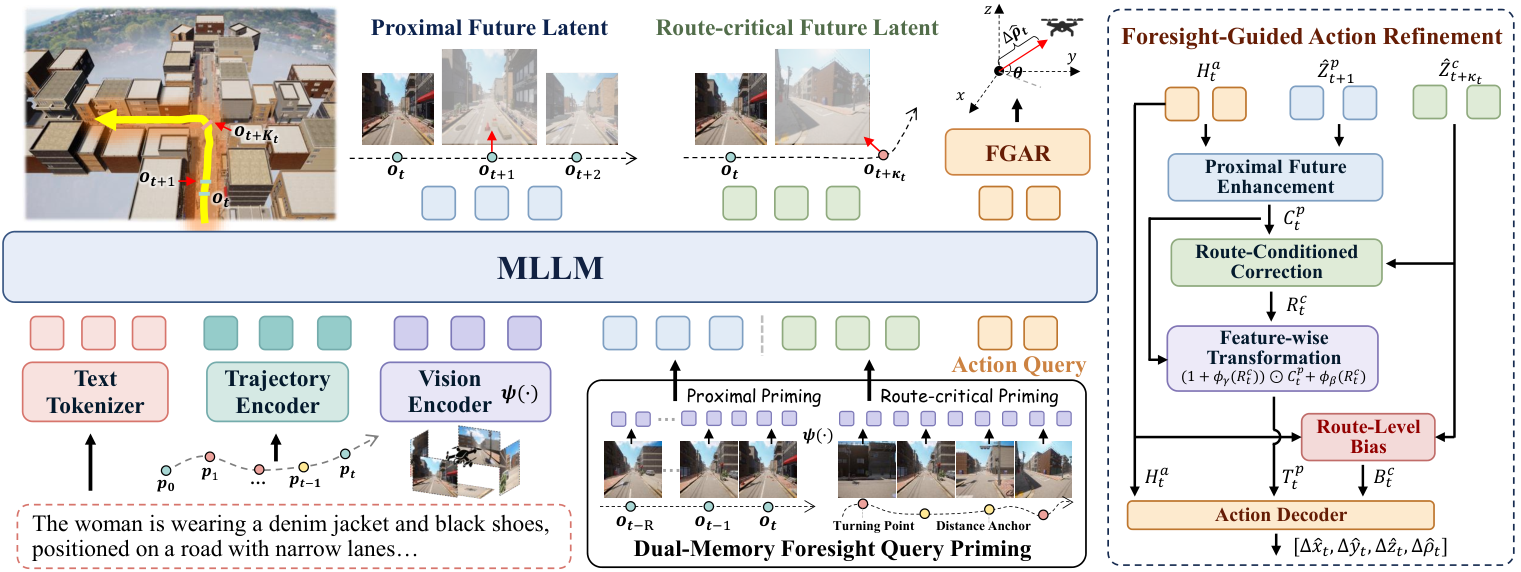
\includegraphics[width=\linewidth,height=22mm,keepaspectratio]{figures/p_forefly.png}\par{\fontsize{6.6}{8}\selectfont\color{muted}ForeFly Fig.2：任务条件未来}\par\endgroup\vspace{1mm}
\end{minipage}\hfill
\begin{minipage}[t]{0.485\linewidth}\vspace{0pt}\raggedright \par\begingroup\centering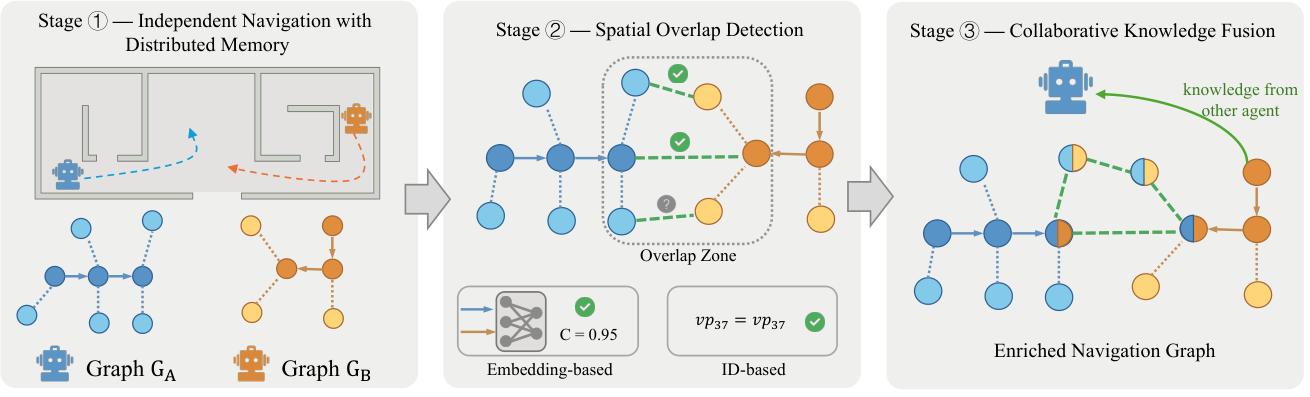
\includegraphics[width=\linewidth,height=22mm,keepaspectratio]{figures/p_covln.png}\par{\fontsize{6.6}{8}\selectfont\color{muted}Co-VLN Fig.2：多智能体记忆共享}\par\endgroup\vspace{1mm}
\end{minipage}\par
\vspace{2mm}
无人机与移动无人系统：技术演进、方法比较与研究设计\par
{\color{muted}\fontsize{8}{10}\selectfont 30篇论文的方法、架构与实验分析 · 2024—2026 · 2026年10月28日}

\note{报告围绕一个技术链条展开：语言任务如何决定要保留的历史、要取得的新视角和要生成的动作；这些能力如何通过运行系统形成闭环，又如何扩展到多机器人。正文对30篇论文分别给出方法页，重点论文进一步分析训练、消融和执行机制。最后根据已有方法提出群体任务条件主动感知方案。}
\end{frame}
\gdef\slidesource{\href{https://arxiv.org/html/2502.18041v7}{[1] OpenFly}；\href{https://arxiv.org/html/2606.14772v1}{[12] ScoutVLA}；\href{https://arxiv.org/html/2605.15964v1}{[16] WorldVLN}；\href{https://arxiv.org/html/2603.12908v2}{[25] GoalSwarm}}
\begin{frame}[t,label=question]{研究主线：任务理解、观察决策与飞行执行}
\relax
\lead{无人系统研究正在把“理解指令、选择观察、生成运动”接成同一个闭环。}{\fontsize{8.5}{10.8}\selectfont\rowcolors{2}{white}{zebra}
\begin{tabularx}{\linewidth}{@{}Y{0.65}Y{1.25}Y{1.1}@{}}\toprule\rowcolor{navy}\thd{技术问题} & \thd{代表论文} & \thd{核心机制}\\\midrule
数据与视觉动作对齐 & OpenFly、TravelUAV、UAV-Flow；AerialVLA、VLA-AN & 关键帧、层级航点、动作编码与渐进训练\\
任务条件主动观察 & USS-Nav、RAVEN、AirHunt、APEX；Scout、ActiveFly、FlyCo & 持久空间记忆、语义搜索、问答取景与表面补全\\
世界预测到运动 & ANWM、WorldFly、ForeFly、WorldVLN、ImagineUAV、DiffWAM & 候选评价、联合生成、特征预测、几何动作读出\\
闭环学习与运行 & RefineFly、EG-GRPO、X-Fly、AeroDASH；两篇RoboHarness & 失败恢复、意图奖励、停止监督、异步接轨与策略交接\\
协作与群体感知 & Air-Ground、GoalSwarm、Co-VLN、SurveilNav、AGC-VLN & 共享地图、前沿竞拍、拓扑融合与跨视角规划\\
\bottomrule\end{tabularx}\par}
\takeaway{研究趋势：观测从模型输入变成可规划资源，动作从单步输出变成带时序和反馈的执行过程。}
\end{frame}
\gdef\slidesource{原文依据：\href{https://arxiv.org/html/2512.15258v2}{[6] VLA-AN}；\href{https://arxiv.org/html/2601.12742v1}{[8] AirHunt}；\href{https://arxiv.org/html/2609.33581v1}{[18] ForeFly}；\href{https://arxiv.org/html/2606.14772v1}{[12] ScoutVLA}}
\begin{frame}[t,label=teams]{代表团队及技术积累}
\relax
{\fontsize{8.7}{11.1}\selectfont
\rowcolors{2}{white}{zebra}
\begin{tabularx}{\linewidth}{@{}Y{0.99}Y{1.02}Y{0.99}@{}}\toprule
\rowcolor{navy}\thd{团队／合作线} & \thd{代表工作} & \thd{技术主线}\\\midrule
浙江大学高飞／周鑫合作线 & VLA-AN、EG-GRPO、DiffWAM & 专家后训练、生成先验、动作读出\\
清华SIGS—南科大STAR & AirHunt、AeroDASH & 搜索确认、慢推理、连续飞行接轨\\
清华等世界模型合作线 & ANWM、WorldVLN、WorldFly、ActiveFly & 动作条件未来、联合生成、观察任务\\
CASIA／国科大／鹏城等 & ForeFly；ImagineUAV为另一合作线 & 双时域预测、视觉运动恢复\\
国防科大—GigaAI & ScoutVLA & 问题驱动取景、语义／动作适配\\
CMU AirLab／UPenn GRASP & RAVEN／Air-Ground & 持久空间证据、真实空地系统\\
\bottomrule\end{tabularx}\par}
\par\ph{两条RoboHarness}\quad 同名但作者不同：一条做策略编排与接管，一条做几何工具与可验证状态；后面分开讲。\par\vspace{1mm}
\takeaway{值得持续跟踪的技术积累：三维空间表征、观察行为学习、世界动作模型和真实闭环系统。}

\note{按技术积累而非论文数量组织团队。浙江大学合作线涉及导航专用训练、专家引导强化学习以及生成表征中的几何运动读出；清华SIGS与南科大STAR相关工作强调语义与几何规划的异步协作；CASIA的ForeFly研究双时域未来特征。CMU的RAVEN和UPenn的空地系统提供空间记忆和真实运行经验。团队归属依论文作者机构，合作关系不等同于共享所有技术实现。}
\end{frame}
\gdef\slidesource{原文依据：\href{https://arxiv.org/html/2502.18041v7}{[1] OpenFly}；\href{https://arxiv.org/html/2410.07087v2}{[2] TravelUAV}；\href{https://arxiv.org/html/2505.15725v2}{[3] UAV-Flow}；\href{https://arxiv.org/html/2506.02896v3}{[4] FlySearch}；\href{https://arxiv.org/html/2601.07558v1}{[14] FlyCo}}
\begin{frame}[t,label=protocol]{任务定义与评价尺度}
\relax
{\fontsize{8.7}{11.1}\selectfont
\rowcolors{2}{white}{zebra}
\begin{tabularx}{\linewidth}{@{}Y{0.69}Y{1.29}Y{1.02}@{}}\toprule
\rowcolor{navy}\thd{任务／基准} & \thd{评价什么} & \thd{协议里必须固定的}\\\midrule
长程VLN：OpenFly／TravelUAV & SR、OSR、SPL、NE & OpenFly停止半径20m；TravelUAV分三级辅助，oracle路线单列\\
原子指令：UAV-Flow & 穿越／环绕等行为完成率 & 和长程搜索不同任务；固定词表与开放词表分开\\
目标搜索：FlySearch／AirHunt & 正确实例与自主结束 & 到过、FOUND、距离阈值、确认条件逐项记录\\
问题取景：Scout／ActiveFly & 可见性、答案、联合成功 & 用固定回答器隔离观察贡献；各表分母不同\\
表面扫描：FlyCo & 几何完整性、无碰撞完成 & 覆盖率不等于语言任务SR；交互时间单列\\
群体任务 & 任一到达／全部完成／证据充分 & 先定事件再跑实验；能量、墙钟、通信分开报\\
\bottomrule\end{tabularx}\par}
\takeaway{长程导航看目标到达，原子飞行看指令执行，主动感知看信息获取，群体任务看共同目标的完成。}

\note{这些论文的成功率分母和成功事件不同。OpenFly采用20米终点阈值并计碰撞失败；UAV-Flow同时评价语义动作和轨迹相似度；FlySearch要求目标入视锥、接近目标并发出FOUND；ScoutVLA则联合评价取景和回答。方法比较主要依据同一论文中的同协议对照，横向比较关注架构和训练机制。}
\end{frame}
\section{数据、表征与单体导航}
\gdef\slidesource{\href{https://arxiv.org/html/2502.18041v7}{[1] OpenFly} · §3–6；Fig.4；Tables 2–3}
\begin{frame}[t,label=openfly]{OpenFly：关键帧记忆与视觉 token 压缩}
\relax
\par\begingroup\centering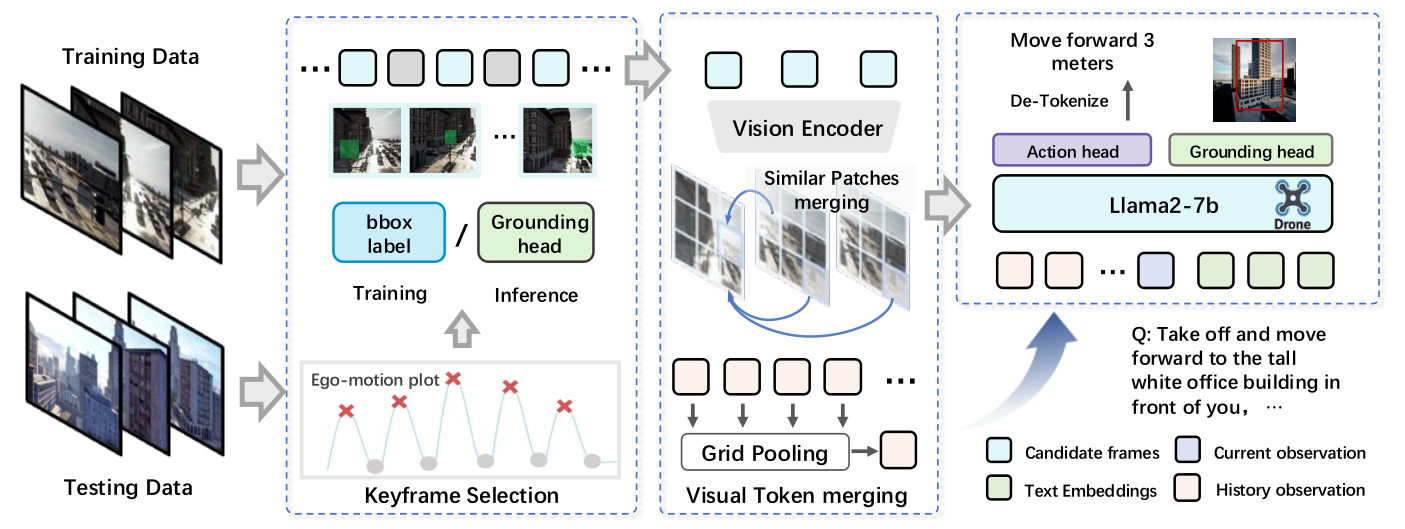
\includegraphics[width=\linewidth,height=27.0mm,keepaspectratio]{figures/p_openfly.png}\par{\fontsize{6.6}{8}\selectfont\color{muted}OpenFly Fig.4：关键帧感知的 OpenFly-Agent}\par\endgroup\vspace{1mm}

\noindent\begin{minipage}[t]{.323\linewidth}\vspace{0pt}\raggedright \ph{问题与输入}\quad 长航程视频高度冗余。以OpenVLA为底座，输入指令、当前图和压缩历史；转向变化与地标显著性共同筛关键帧。\par\end{minipage}\hfill\begin{minipage}[t]{.323\linewidth}\vspace{0pt}\raggedright \ph{架构与训练}\quad 三层cross-attention预测地标框；大框图作参考，跨帧相似token合并，再做grid pooling。当前图保留256 token，历史库容量2。\par\end{minipage}\hfill\begin{minipage}[t]{.323\linewidth}\vspace{0pt}\raggedright \ph{实验发现}\quad 18场景、100K轨迹。Seen / Unseen SR为34.3 / 22.6；均匀历史＋合并16.6，关键帧＋合并34.3（Seen）。\par\end{minipage}
\takeaway{方法要点：历史选择与压缩必须配合，突出地标事件比平均保存所有过去画面更有效。}
\note{数据工具链连接UE、GTA V、Google Earth和3DGS，统一位姿控制、图像和点云获取接口，自动完成语义实例、轨迹和指令生成。OpenFly-Agent的地标框使用训练工具链产生的框做GIoU监督；推理时由网络预测框。候选关键帧来自运动变化及其相邻帧，并由框面积阈值筛选。参考图选择地标框最大者，以余弦相似度合并跨帧token，历史再做网格池化，保留当前图的细节。Table3中单独关键帧SR9.2，单独均匀历史与合并16.6，二者结合34.3，说明有效历史表征是系统收益的关键。}
\end{frame}
\gdef\slidesource{\href{https://arxiv.org/html/2410.07087v2}{[2] TravelUAV / OpenUAV} · §5–7；Fig.3；Tables 2–3}
\begin{frame}[t,label=traveluav]{TravelUAV：语义目标姿态与局部轨迹分层解码}
\relax
\par\begingroup\centering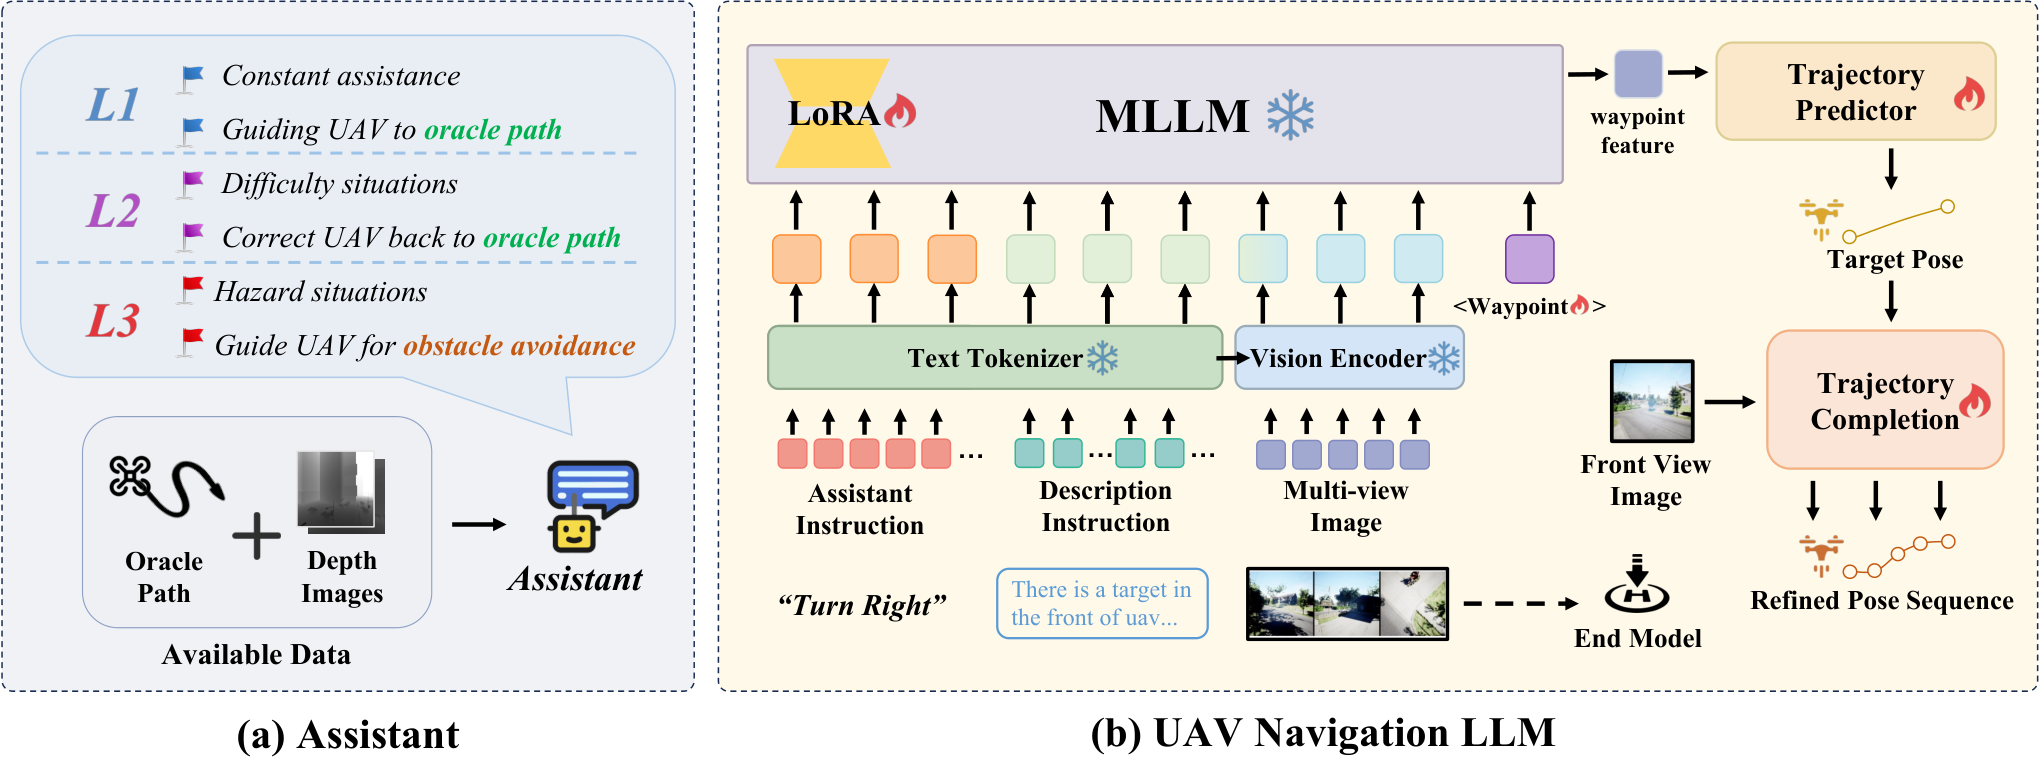
\includegraphics[width=\linewidth,height=28mm,keepaspectratio]{figures/p_traveluav.png}\par{\fontsize{6.6}{8}\selectfont\color{muted}TravelUAV Fig.3：辅助机制与 UAV Navigation LLM}\par\endgroup\vspace{1mm}

\noindent\begin{minipage}[t]{.323\linewidth}\vspace{0pt}\raggedright \ph{任务与数据}\quad OpenUAV提供22类场景、12,149条轨迹。目标描述与五视角RGB-D、飞行状态输入模型，生成连续位姿序列。\par\end{minipage}\hfill\begin{minipage}[t]{.323\linewidth}\vspace{0pt}\raggedright \ph{层级架构}\quad EVA-CLIP＋Q-former编码视觉，Vicuna-7B融合指令；可学习轨迹query先预测远端目标姿态，再结合前视特征细化局部轨迹。\par\end{minipage}\hfill\begin{minipage}[t]{.323\linewidth}\vspace{0pt}\raggedright \ph{学习与效果}\quad 回溯采样聚合偏航后的恢复样本。L1下Seen SR由16.10升至17.45；辅助等级L1 / L2 / L3分别提供不同强度的导航纠正。\par\end{minipage}
\takeaway{方法要点：用语义模型选远端状态，用局部视觉补轨迹细节，并从实际偏航状态补恢复监督。}
\note{TravelUAV是方法与基准的常用简称，完整题名为Towards Realistic UAV Vision-Language Navigation: Platform, Benchmark, and Methodology。视觉图像分别压成1个全局context token与16个局部content token，轨迹query从多模态LLM中提取目标姿态特征，局部解码器再结合前视视觉生成细轨迹。训练中的回溯采样在失败或偏移状态重新连接参考路径，缓解只学专家状态的分布偏移。原任务区分L1高频路径辅助、L2偏离或危险时辅助、L3仅避障辅助。这里17.45对应L1加数据聚合；这种分层结构为后续世界动作模型提供了可替换的目标姿态与局部运动接口。}
\end{frame}
\gdef\slidesource{\href{https://arxiv.org/html/2505.15725v2}{[3] UAV-Flow} · §2–4；Fig.6；Appendix B}
\begin{frame}[t,label=uavflow]{UAV-Flow：把语言对齐到细粒度飞行行为}
\relax
\par\begingroup\centering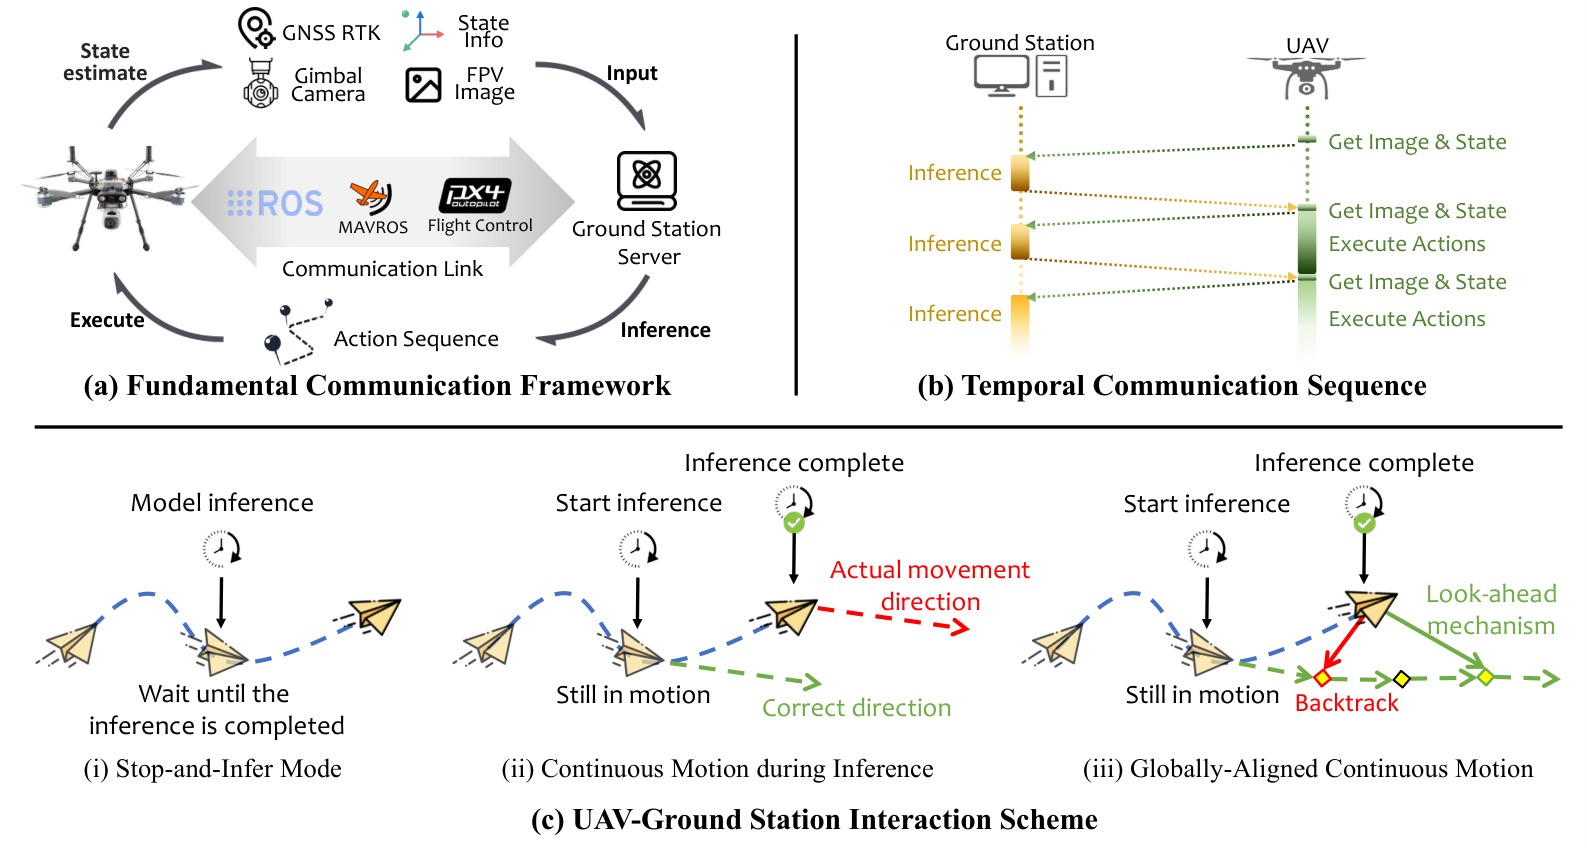
\includegraphics[width=\linewidth,height=28mm,keepaspectratio]{figures/p_uavflow.png}\par{\fontsize{6.6}{8}\selectfont\color{muted}UAV-Flow Fig.6：地面推理与无人机连续执行}\par\endgroup\vspace{1mm}

\noindent\begin{minipage}[t]{.323\linewidth}\vspace{0pt}\raggedright \ph{研究问题}\quad 将“绕过、穿越、环绕、悬停”等短程指令映射为飞行动作。数据含30K真实与10K仿真轨迹，覆盖10类主要运动。\par\end{minipage}\hfill\begin{minipage}[t]{.323\linewidth}\vspace{0pt}\raggedright \ph{建模方式}\quad 按5Hz对齐图像与6-DoF状态，设固定和开放指令集。OpenVLA以离散token输出位姿；\ensuremath{\pi}0用flow matching生成动作块。\par\end{minipage}\hfill\begin{minipage}[t]{.323\linewidth}\vspace{0pt}\raggedright \ph{执行与评价}\quad 地面站推理返回局部目标，结合采样位姿转为全局参考，剔除已越过点；用语义SR与nDTW同时评价行为和路径。\par\end{minipage}
\takeaway{方法要点：同一句指令可以对应多条合理轨迹；动作意图、视觉目标和执行时延必须一起处理。}
\note{UAV-Flow的贡献主要是任务定义、真实飞行数据和统一部署基准。真实数据由专业飞手在三个校园采集，先将GPS和姿态变为起始局部坐标，再按时间插值对齐视频；固定模板经语言扩写形成开放词表。基线适配包括将传统VLN分类头换成连续位姿回归，以及给\ensuremath{\pi}0加入初始和当前双帧输入。Globally-Aligned Continuous Motion将查询时刻的预测与实际执行状态关联，并过滤已走过目标，减少通信和推理延迟造成的控制错位。后续ImagineUAV和AeroDASH都沿用这类短程动作任务。}
\end{frame}
\gdef\slidesource{\href{https://arxiv.org/html/2506.02896v3}{[4] FlySearch} · §3–4；Tables 2、4}
\begin{frame}[t,label=flysearch]{FlySearch：在闭环搜索中检验视觉空间推理}
\relax
\par\begingroup\centering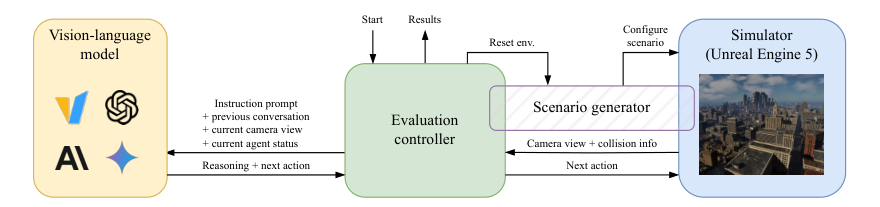
\includegraphics[width=\linewidth,height=28mm,keepaspectratio]{figures/p_flysearch.png}\par{\fontsize{6.6}{8}\selectfont\color{muted}FlySearch Fig.2：场景生成、模型决策与闭环评价}\par\endgroup\vspace{1mm}

\noindent\begin{minipage}[t]{.323\linewidth}\vspace{0pt}\raggedright \ph{输入与动作}\quad 俯视RGB图叠坐标网格并给高度；VLM直接输出米制相对位移或FOUND，自动驾驶器负责基本运动与碰撞阻断。\par\end{minipage}\hfill\begin{minipage}[t]{.323\linewidth}\vspace{0pt}\raggedright \ph{任务设计}\quad FS-1检验接近和识别，FS-Anomaly-1检验异常语义，FS-2扩大搜索空间。正确FOUND要求目标在视锥内且高度差不超过10m。\par\end{minipage}\hfill\begin{minipage}[t]{.323\linewidth}\vspace{0pt}\raggedright \ph{实验发现}\quad FS-1中Gemini 2.0 Flash为42.0\%，FS-2仅6.0\%；FS-1从10步增至20步，整体SR由42.0降至39.5。\par\end{minipage}
\takeaway{研究发现：增加动作机会仍会因空间记忆和停止判断出错而失效，闭环信息利用比单张图理解更难。}
\note{FlySearch通过UE5程序化生成城市和森林环境，以控制器连接多模态模型和模拟器；模型使用可解析XML描述相对位移。FS-1初始视锥覆盖目标，但目标可能因尺度太小而难辨认，因此主要考验缩放、接近与识别；FS-2不要求初始可见，真正扩大探索负担。实验对比显示主流VLM在FS-2远低于人类60.8\%参考，FS-1的人类参考为66.7\%。多步预算实验说明探索链越长，重复访问、误认和未及时FOUND的错误越容易累积。}
\end{frame}
\gdef\slidesource{\href{https://arxiv.org/html/2603.14363v1}{[5] AerialVLA} · §3–4；Tables 2–4；固定v1}
\begin{frame}[t,label=aerialvla]{AerialVLA：双视角输入与统一导航／降落输出}
\relax
\par\begingroup\centering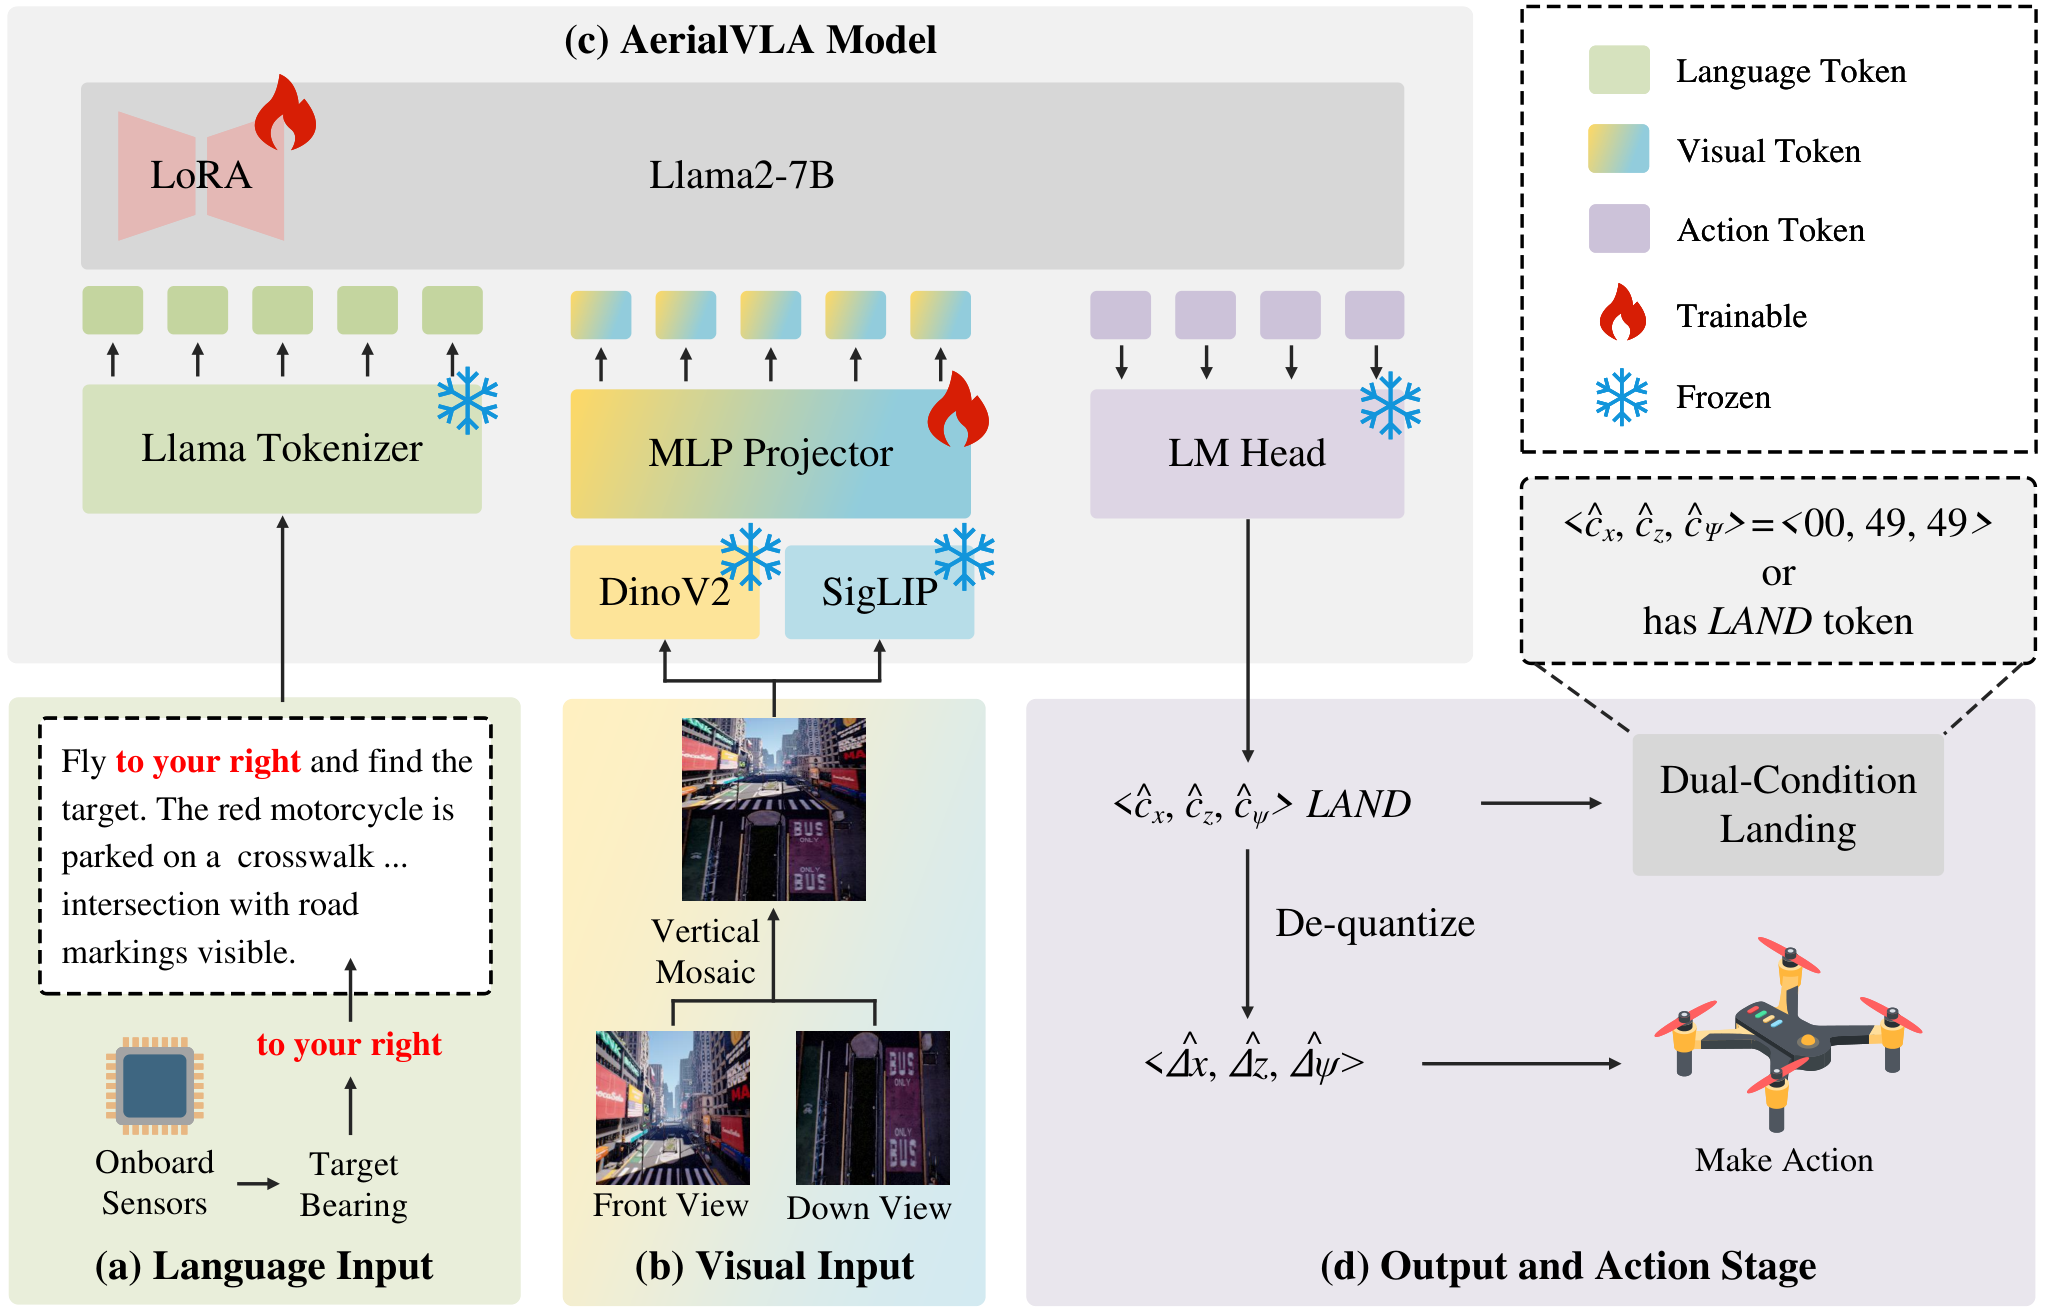
\includegraphics[width=\linewidth,height=28mm,keepaspectratio]{figures/p_aerialvla.png}\par{\fontsize{6.6}{8}\selectfont\color{muted}AerialVLA Fig.2：视觉、方向提示与数值动作编码}\par\endgroup\vspace{1mm}

\noindent\begin{minipage}[t]{.323\linewidth}\vspace{0pt}\raggedright \ph{核心思路}\quad 减少模块间语义断层。前视图负责前进与目标识别，下视图负责对准和降落；两图拼接后送入SigLIP＋DINOv2与LLaMA 2。\par\end{minipage}\hfill\begin{minipage}[t]{.323\linewidth}\vspace{0pt}\raggedright \ph{输出与训练}\quad 粗方向提示代替逐步路径辅助；自回归输出前向、垂向、yaw三类控制及LAND。冻结视觉编码器，训练投影层与LoRA。\par\end{minipage}\hfill\begin{minipage}[t]{.323\linewidth}\vspace{0pt}\raggedright \ph{结果与分析}\quad TravelUAV Seen / 未见对象 / 未见地图SR为47.96 / 56.60 / 37.58\%。反应式控制简洁，显式记忆由后续方法扩展。\par\end{minipage}
\takeaway{方法要点：把“什么时候结束”纳入同一策略学习，使视觉到控制的路径更短。}
\note{本页采用AerialVLA的arXiv v1；作者项目后续使用AeroVLA名称。模型将前视和下视竖直拼接为224×224输入，以语义和几何互补的双视觉编码器提取特征。方向提示将相对目标方位分成直行、左右前方、左右和左右后方等桶；因此系统仍使用目标方位先验。数值动作token经反归一化成为连续控制，LAND或近零位移触发终止。训练包含几何一致性筛选，以排除无障碍但方向提示与示范动作相冲突的样本。结果对应论文自己的协议与引用基线；架构启示在于统一动作与终止，而跨论文效果比较仍需匹配辅助条件。}
\end{frame}
\gdef\slidesource{\href{https://arxiv.org/html/2512.15258v2}{[6] VLA-AN} · §3.2–3.5；Fig.2；Tables 2–3}
\begin{frame}[t,label=vlaan]{VLA-AN：渐进训练与几何约束动作模块}
\relax
\par\begingroup\centering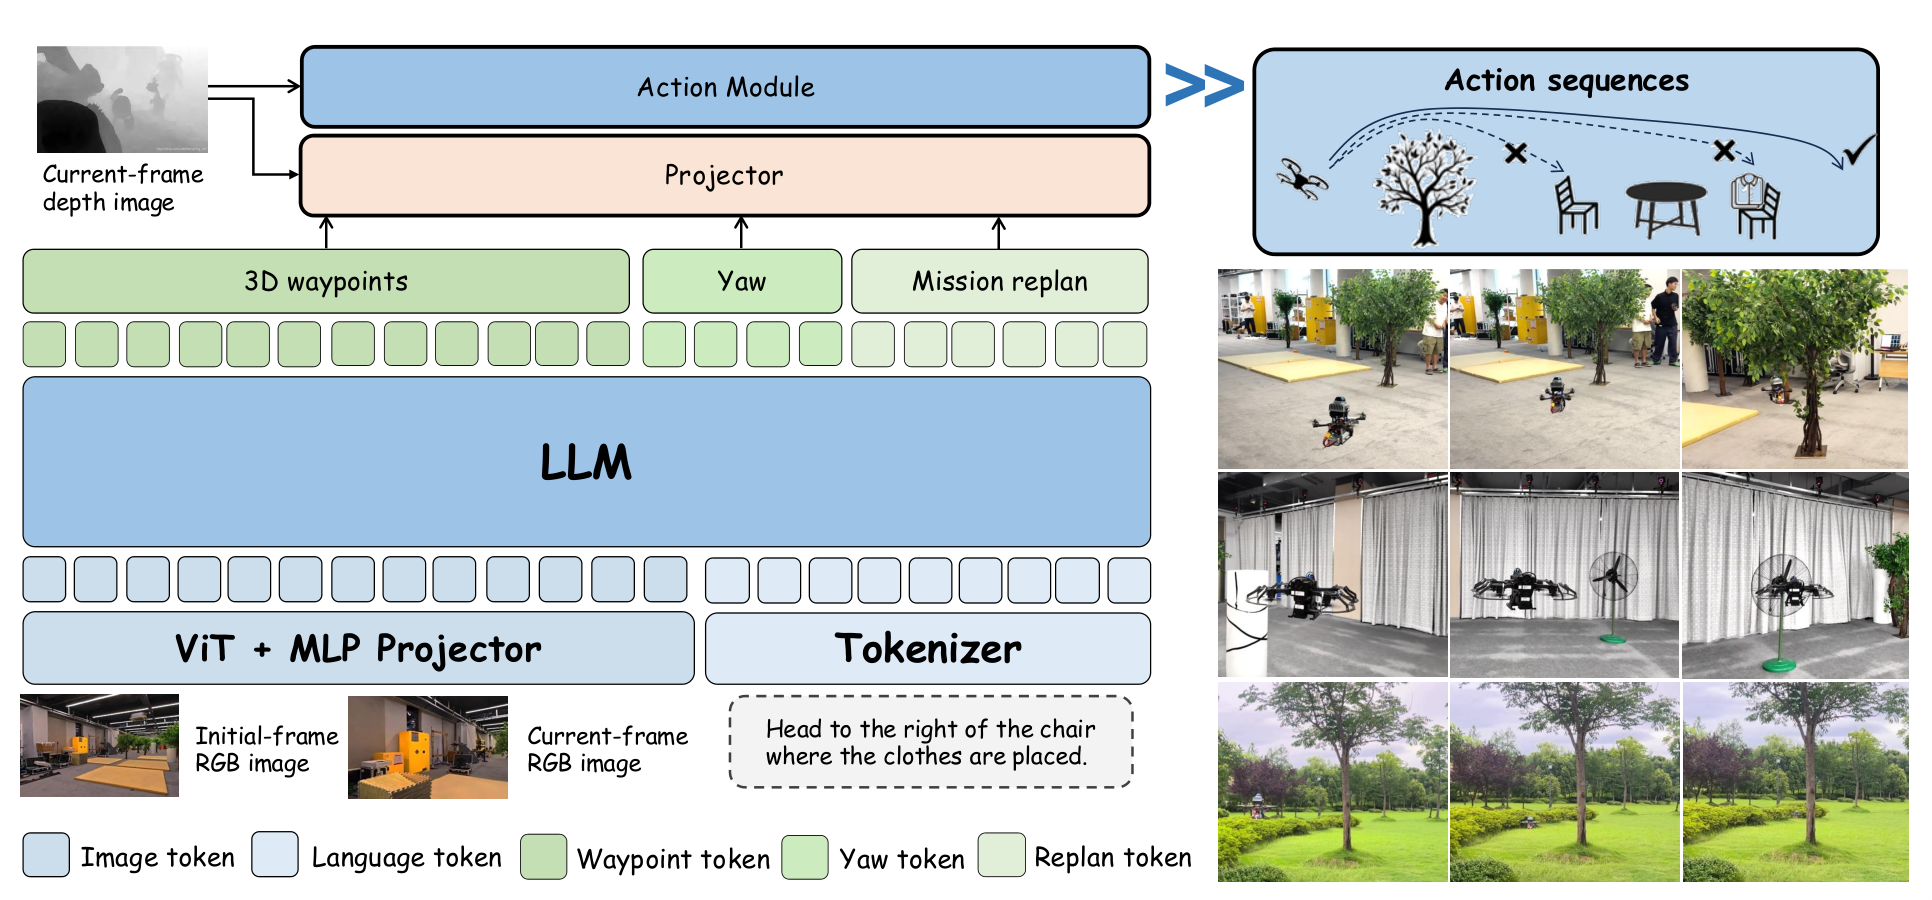
\includegraphics[width=\linewidth,height=28mm,keepaspectratio]{figures/p_vlaan.png}\par{\fontsize{6.6}{8}\selectfont\color{muted}VLA-AN Fig.2：多模态推理与鲁棒动作模块}\par\endgroup\vspace{1mm}

\noindent\begin{minipage}[t]{.323\linewidth}\vspace{0pt}\raggedright \ph{任务与表征}\quad 将目标实体、属性和空间关系解析为3D航点及yaw；初始／当前视图比较任务进度，形成导航—重规划—完成状态机。\par\end{minipage}\hfill\begin{minipage}[t]{.323\linewidth}\vspace{0pt}\raggedright \ph{模型与执行}\quad ViT、投影层与LLM负责语义到目标；动作模块将目标变成轨迹，碰撞段由深度几何提供斥力修正，并重新分配执行时间。\par\end{minipage}\hfill\begin{minipage}[t]{.323\linewidth}\vspace{0pt}\raggedright \ph{数据与部署}\quad 3DGS真实重建＋可编辑mesh混合数据；三阶段学习推理、导航及GRPO。Orin NX进行量化和推理优化，报告2–3Hz闭环。\par\end{minipage}
\takeaway{方法要点：航点作为跨数据、跨平台的中间接口，语义学习与局部轨迹约束各自发挥作用。}
\note{VLA-AN完整题名为An Efficient and Onboard Vision-Language-Action Framework for Aerial Navigation in Complex Environments。自动数据管线将真实视频重建为3DGS场景并导入Unity，人工给任务元数据后随机化起终点，用动力学规划生成飞行示范，按10Hz同步多视图、深度和位姿。模型输出语义航点而非电机命令，有利于复用不同机器人导航经验。动作模块对与障碍相交的参考轨迹构造几何表面锚和斥力梯度，修正后重估时间以满足运动约束。部署优化包括AWQ、注意力和算子融合、KV cache以及CUDA graph。}
\end{frame}
\gdef\slidesource{\href{https://arxiv.org/html/2512.15258v2}{[6] VLA-AN} · §3.3；Table 3（SR，\%）}
\begin{frame}[t,label=vlaan_training]{VLA-AN：先保留推理能力，再注入导航与奖励}
\relax
\bline{阶段I：理解与推理}{通用VQA、空间grounding、推理和多帧数据做全参数SFT，建立实体、空间关系与场景理解。}
\bline{阶段II：导航专门化}{加入高质量飞行示范，同时混入VQA，学习3D航点、yaw与重规划，并维持语义推理。}
\bline{阶段III：GRPO}{对多候选回答做组内相对优化；答案匹配、空间IoU及输出格式提供奖励，强化指令与空间约束的对齐。}{\fontsize{8.5}{10.8}\selectfont\rowcolors{2}{white}{zebra}
\begin{tabularx}{\linewidth}{@{}Y{1.2}Y{0.95}Y{0.95}Y{0.95}Y{0.95}@{}}\toprule\rowcolor{navy}\thd{Table 3配置} & \thd{场景推理} & \thd{空间grounding} & \thd{对象导航} & \thd{长程导航}\\\midrule
基线 & 77.4 & 68.2 & 34.2 & 20.4\\
导航SFT & 75.6 & 64.3 & 95.3 & 74.9\\
两阶段SFT & 82.3 & 91.1 & 92.9 & 72.2\\
完整训练 & 85.5 & 94.6 & 98.1 & 85.7\\
\bottomrule\end{tabularx}\par}
\takeaway{导航数据决定行动能力，通用推理数据与奖励训练帮助保留复杂任务所需的语义能力。}
\note{Table3给出四类能力的训练消融。仅导航训练对象导航95.3、长程74.9，但场景推理与空间grounding低于加入通用理解训练的配置；完整训练在导航与空间任务上取得更好平衡。这里98.1是该表完整模型的对象导航SR，Table2不同数据配方出现99.2，二者分别属于训练策略与数据构成消融，不合并成一个统一结果。}
\end{frame}
\section{空间记忆与主动感知}
\gdef\slidesource{文献分析：\href{https://arxiv.org/html/2602.00708v2}{[7] USS-Nav}；\href{https://arxiv.org/html/2509.23563v1}{[10] RAVEN}；\href{https://arxiv.org/html/2601.12742v1}{[8] AirHunt}}
\begin{frame}[t,label=persistent]{持久空间记忆：几何、语义与任务状态}
\relax
{\fontsize{8.7}{11.1}\selectfont
\rowcolors{2}{white}{zebra}
\begin{tabularx}{\linewidth}{@{}Y{0.6}Y{1.08}Y{1.12}Y{1.2}@{}}\toprule
\rowcolor{navy}\thd{方法} & \thd{状态怎样保存} & \thd{如何驱动行动} & \thd{表征的作用}\\\midrule
USS-Nav & 自由空间—区域—对象层级图 & 语义选区域，几何分配可达前沿 & 层级空间结构压缩全局规划\\
RAVEN & 近端语义体素＋远端方向射线 & 行为树切换定位、探查与回退 & 远处方向引导与近处定位衔接\\
AirHunt & 覆盖帧／目标帧＋三维值图 & 区域搜索与实例核验分工 & 区域偏好与目标确认独立更新\\
\bottomrule\end{tabularx}\par}
\par\ph{共同机制}\quad 三者都把一次观察写进可追溯的空间状态：哪里看过、看到什么、还缺什么。下一步动作由“缺什么”决定，而不是由“哪里没去过”决定。\par\vspace{1mm}
\par\ph{群体启示}\quad 交换时带上测量类型、来源、捕获时间、坐标精度和支持的命题。带来源的空间记录支持队友复查与状态更新。\par\vspace{1mm}
\takeaway{三条路线分别压缩空间拓扑、远近语义和任务线索，使历史观察能持续影响下一步动作。}

\note{USS-Nav将局部栅格、全局自由空间拓扑、区域及对象统一在场景图中；RAVEN同时保留深度覆盖内的语义体素和深度外的语义射线；AirHunt用带位姿的关键帧把语义值写入三维地图。三者分别回答全局怎么走、远处往哪找、任务相关区域优先看哪里。下面逐篇分析这些状态如何建立、更新并驱动行动。}
\end{frame}
\gdef\slidesource{\href{https://arxiv.org/html/2602.00708v2}{[7] USS-Nav} · §IV–VI；Figs.2–5}
\begin{frame}[t,label=ussnav]{USS-Nav：自由空间骨架上的层级语义决策}
\relax
\par\begingroup\centering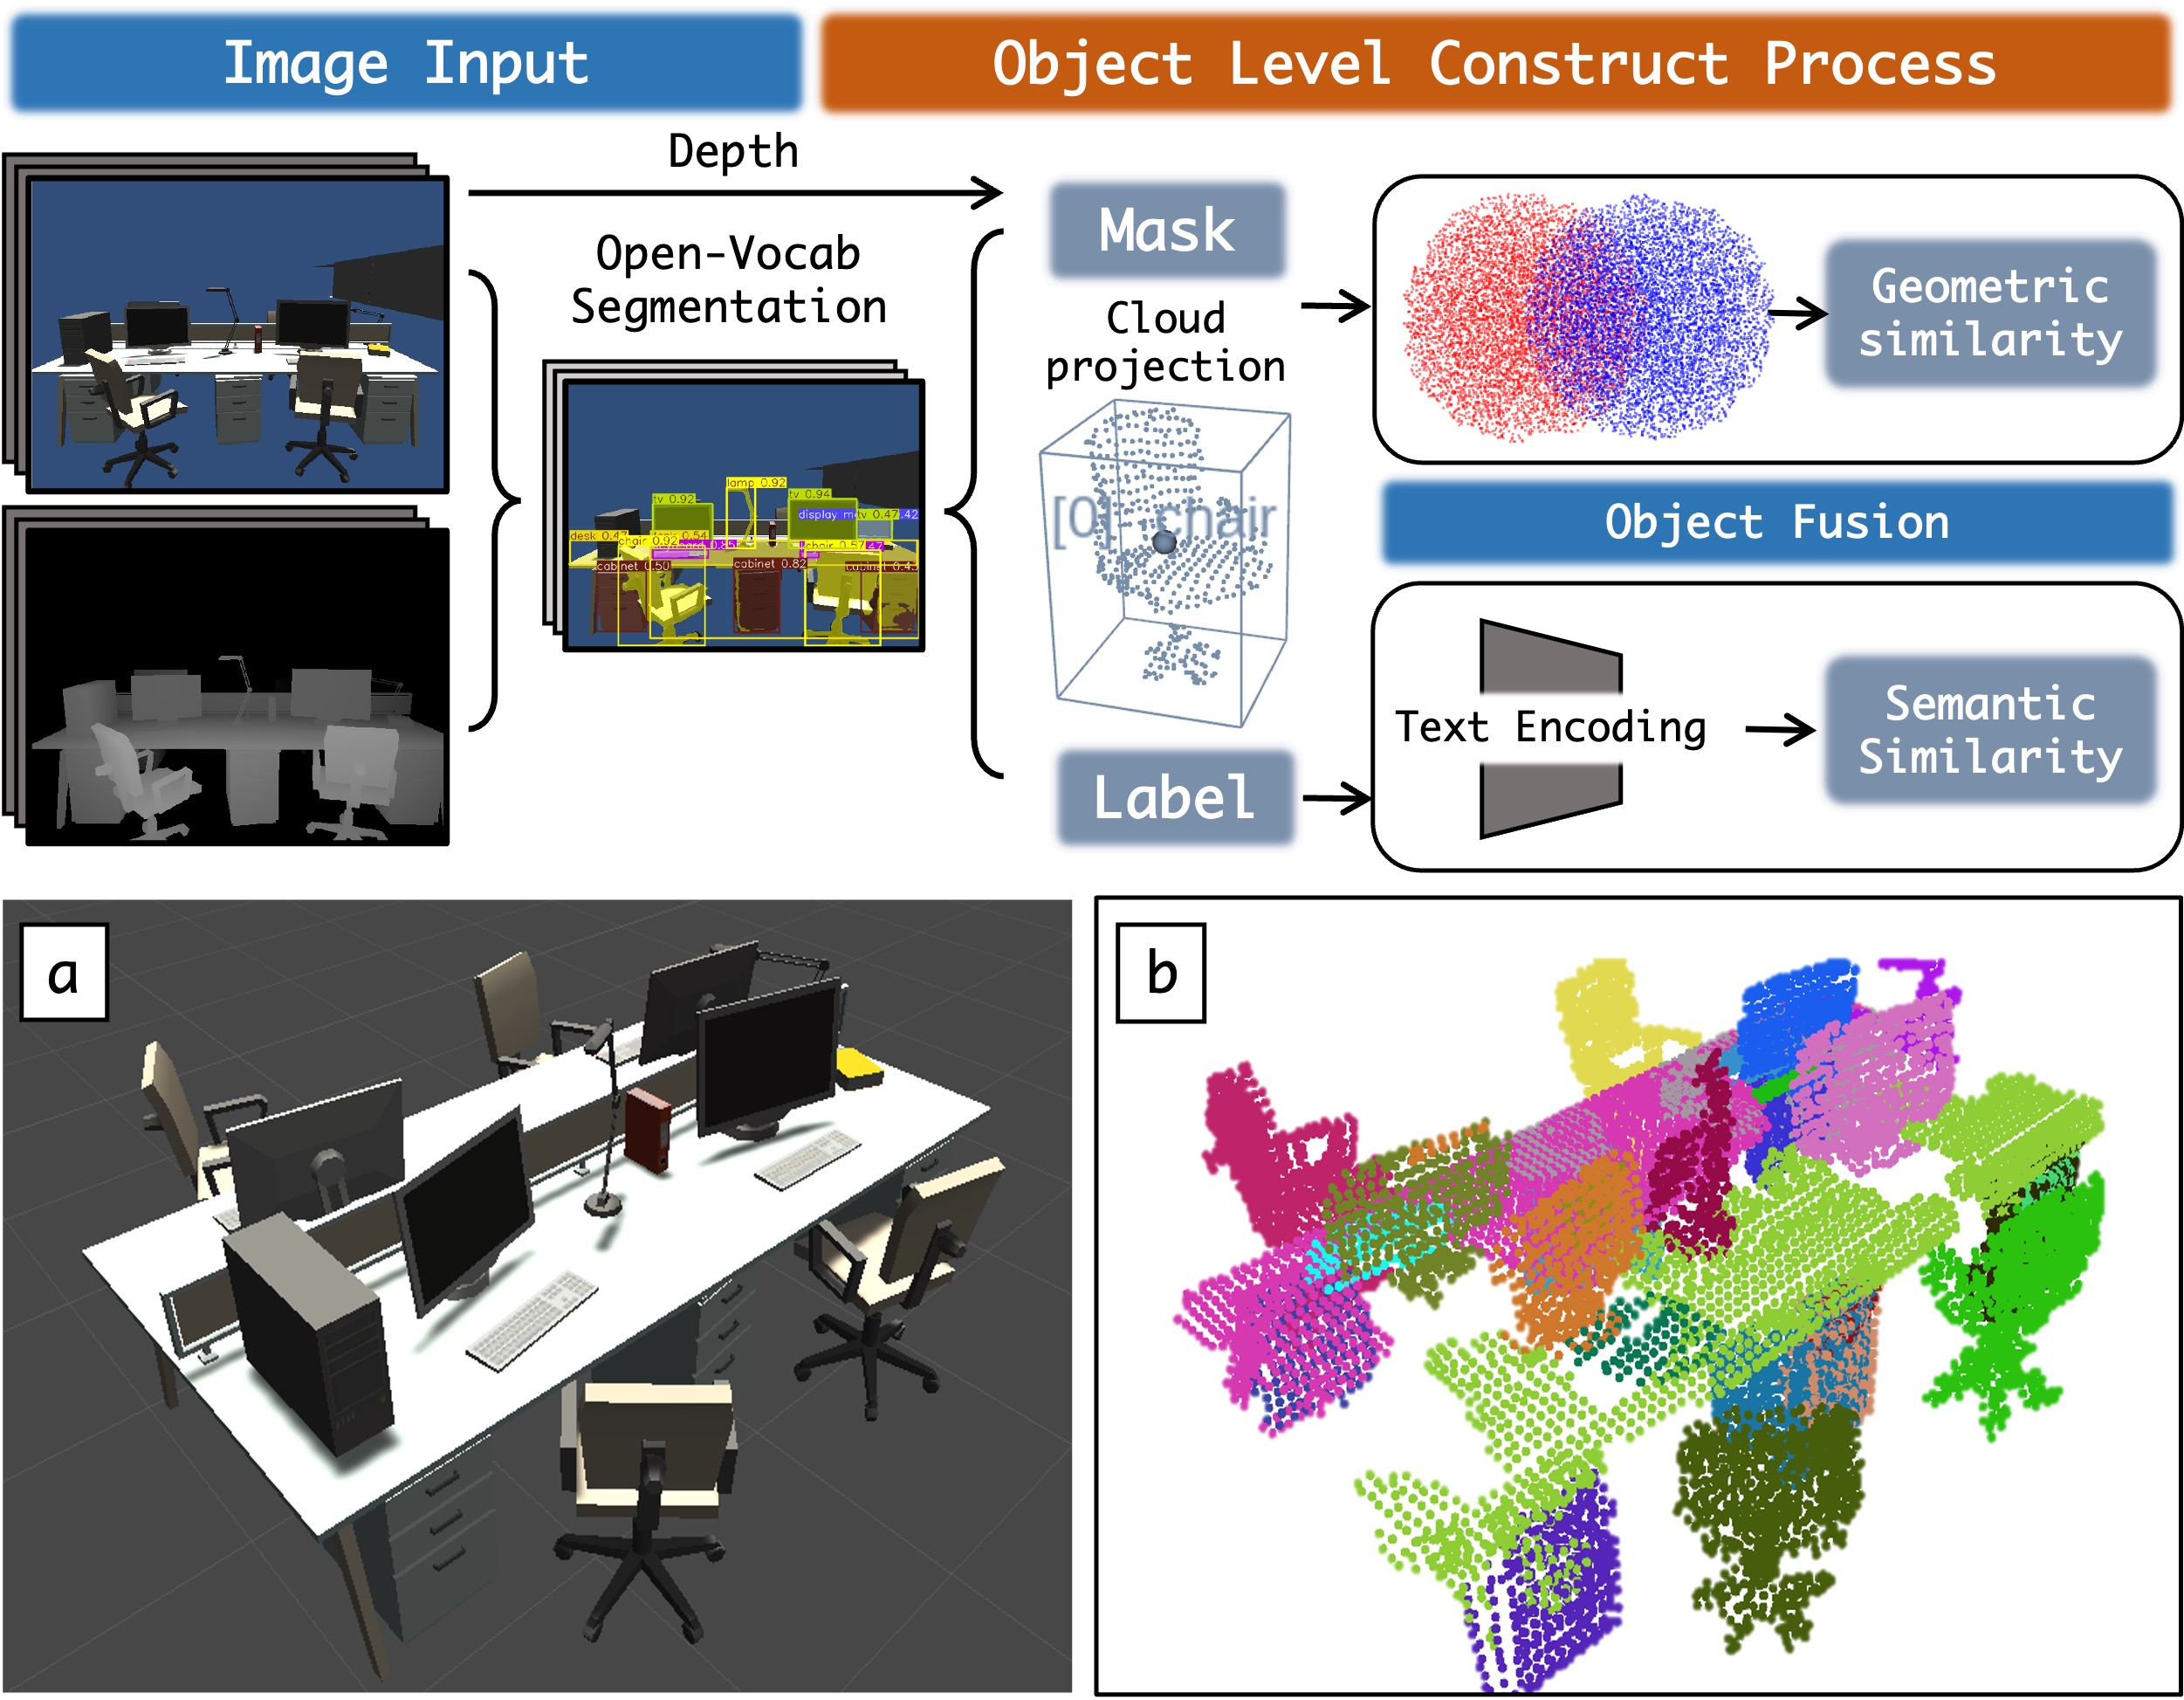
\includegraphics[width=\linewidth,height=28mm,keepaspectratio]{figures/p_ussnav.jpg}\par{\fontsize{6.6}{8}\selectfont\color{muted}USS-Nav Fig.4：几何一致的对象关联与语义实例化}\par\endgroup\vspace{1mm}

\noindent\begin{minipage}[t]{.323\linewidth}\vspace{0pt}\raggedright \ph{空间骨架}\quad 滚动占据栅格中扩张自由空间多面体，以父子、相交与可见关系增量连图；Leiden局部聚类得到稳定的语义区域。\par\end{minipage}\hfill\begin{minipage}[t]{.323\linewidth}\vspace{0pt}\raggedright \ph{对象与决策}\quad YOLO-E分割、深度反投影，按几何重叠及Mobile-CLIP相似度关联对象；LLM粗选区域，TSP安排区域内前沿访问。\par\end{minipage}\hfill\begin{minipage}[t]{.323\linewidth}\vspace{0pt}\raggedright \ph{效率来源}\quad GCM保存历史覆盖，避免局部地图滚动后重复探索；8×8×4m局部图、0.1m分辨率，Orin NX地图更新约15Hz。\par\end{minipage}
\takeaway{方法要点：以稀疏可达拓扑承载语义，使语言推理在区域尺度工作，几何搜索在局部尺度工作。}
\note{多面体以当前自由空间为种子，沿边界继续扩张，将几何连接和历史运动产生的弱连接分开赋权。区域更新只重聚类新节点及相关相邻区域，保持远处区域ID稳定。对象关联先在ikd-tree内检索2米邻域，再综合语义相似度和双向点云重叠进行合并。全局覆盖掩码记录固定空间块中的未知体素量，将已覆盖块从前沿候选中排除。LLM通过区域和对象描述选择目标区域，区域内调用TSP与几何路径规划。15Hz对应地图更新；Qwen-3推理使用外部API。}
\end{frame}
\gdef\slidesource{\href{https://arxiv.org/html/2509.23563v1}{[10] RAVEN} · §III–V；Tables I–II}
\begin{frame}[t,label=raven]{RAVEN：语义射线把远处线索接到近端定位}
\relax
\par\begingroup\centering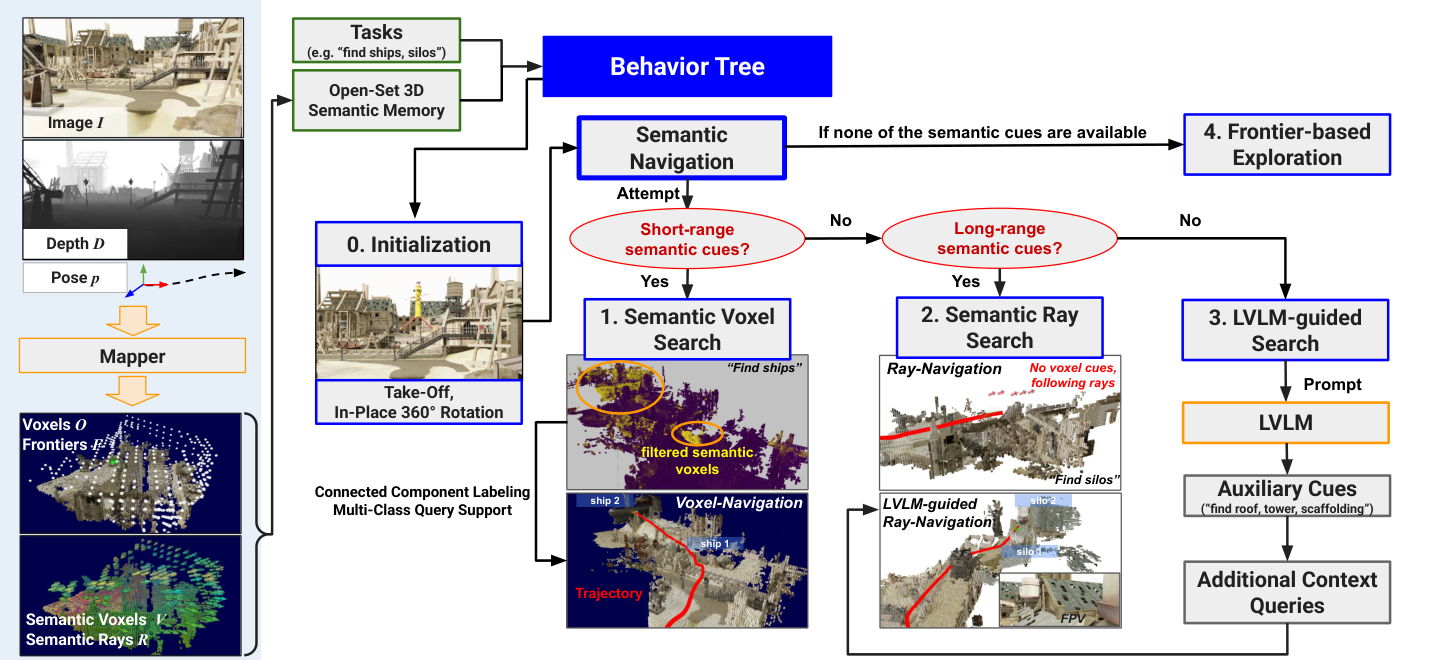
\includegraphics[width=\linewidth,height=28mm,keepaspectratio]{figures/p_raven.png}\par{\fontsize{6.6}{8}\selectfont\color{muted}RAVEN Fig.2：voxel-ray记忆与自适应行为树}\par\endgroup\vspace{1mm}

\noindent\begin{minipage}[t]{.323\linewidth}\vspace{0pt}\raggedright \ph{远近双表征}\quad RGB特征投影到有深度的近端体素；超出深度范围的可见语义保存为带原点与方向的射线，支持之后更换查询目标。\par\end{minipage}\hfill\begin{minipage}[t]{.323\linewidth}\vspace{0pt}\raggedright \ph{行为切换}\quad 先查相关体素，缺近端定位则沿语义射线接近；无线索时使用LVLM辅助地标或几何前沿，逐步转入精确目标搜索。\par\end{minipage}\hfill\begin{minipage}[t]{.323\linewidth}\vspace{0pt}\raggedright \ph{实验发现}\quad 100任务总体Progress / PPL为50.14 / 31.89\%；仅体素14.63，仅射线34.47，体素＋射线无LVLM为47.85。\par\end{minipage}
\takeaway{方法要点：把远处“看见过但测不准”的语义保存为方向线索，接近后再升级为可定位对象。}
\note{RAVEN基于RayFronts编码与SIGLIP对齐，地图不预绑定当前目标类别，因此新任务能重新查询既有记忆。体素按语义相似度筛选后做连通域聚类；射线按角度分桶，综合接近性和密度选方向。行为树把前沿探索、语义体素、语义射线与稀疏LVLM调用接成可回退流程。消融显示在大尺度室外场景中远端射线贡献明显，体素提供接近后的准确定位。真实平台使用AGX Orin和ZED X，地图4.8Hz；实机未接入LVLM分支。Progress衡量多实例目标完成进度，PPL进一步结合路径长度。}
\end{frame}
\gdef\slidesource{原文依据：\href{https://arxiv.org/html/2601.12742v1}{[8] AirHunt}}
\begin{frame}[t,label=airhunt]{AirHunt：语义搜索与几何确认分工}
\relax
\par\begingroup\centering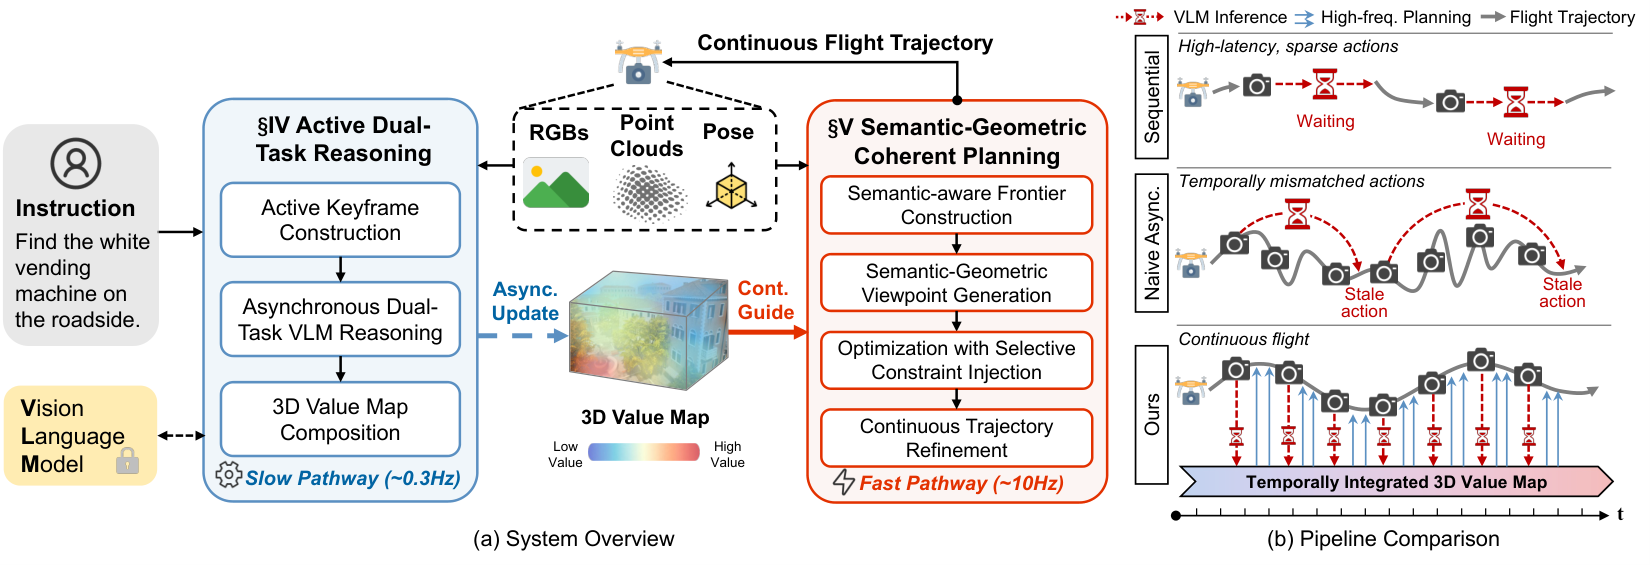
\includegraphics[width=\linewidth,height=30mm,keepaspectratio]{figures/p_airhunt.png}\par{\fontsize{6.6}{8}\selectfont\color{muted}AirHunt · 2（论文原图）}\par\endgroup\vspace{1mm}

\noindent\begin{minipage}[t]{0.3233333333333333\linewidth}\vspace{0pt}\raggedright \par\ph{状态与推理}\quad 覆盖关键帧管区域语义，ADTR任务关键帧管候选目标；Qwen-VL-Max结果带采样位姿写进三维值图，慢线程不直接控飞机。\par\vspace{1mm}
\end{minipage}\hfill
\begin{minipage}[t]{0.3233333333333333\linewidth}\vspace{0pt}\raggedright \par\ph{行动与反馈}\quad 前沿按语义排序，访问顺序再做全局优化；局部轨迹连续飞，新观测回来就更新候选和确认状态。\par\vspace{1mm}
\end{minipage}\hfill
\begin{minipage}[t]{0.3233333333333333\linewidth}\vspace{0pt}\raggedright \par\ph{数据与效果}\quad AirSim，LiDAR 10m、三路$90^{\circ}\times60^{\circ}$相机；85任务\ensuremath{\times}3次，5m阈值、50次Qwen-VL调用；SR/\allowbreak{}OSR/\allowbreak{}SPL=73.1/\allowbreak{}80.5/\allowbreak{}42.0。\par\vspace{1mm}
\end{minipage}\par
\takeaway{架构核心：低频VLM生成语义地图，高频规划持续飞行；地图承担跨频率的信息交接。}

\note{AirHunt的关键是把语义和几何拆成两条线程：VLM在关键帧上给区域和候选目标打分，结果带着采样位姿写进三维值图；前沿排序和轨迹优化仍由几何层完成，所以慢模型不会卡住飞控。85个任务各跑3次，5米搜索半径、50次VLM调用，SR/OSR/SPL分别是73.1/80.5/42.0。}
\end{frame}
\gdef\slidesource{原文依据：\href{https://arxiv.org/html/2601.12742v1}{[8] AirHunt}}
\begin{frame}[t,label=airhunt_detail]{AirHunt：覆盖关键帧、目标关键帧与全局访问顺序}
\relax

\noindent\begin{minipage}[t]{0.49\linewidth}\vspace{0pt}\raggedright \par\begingroup\centering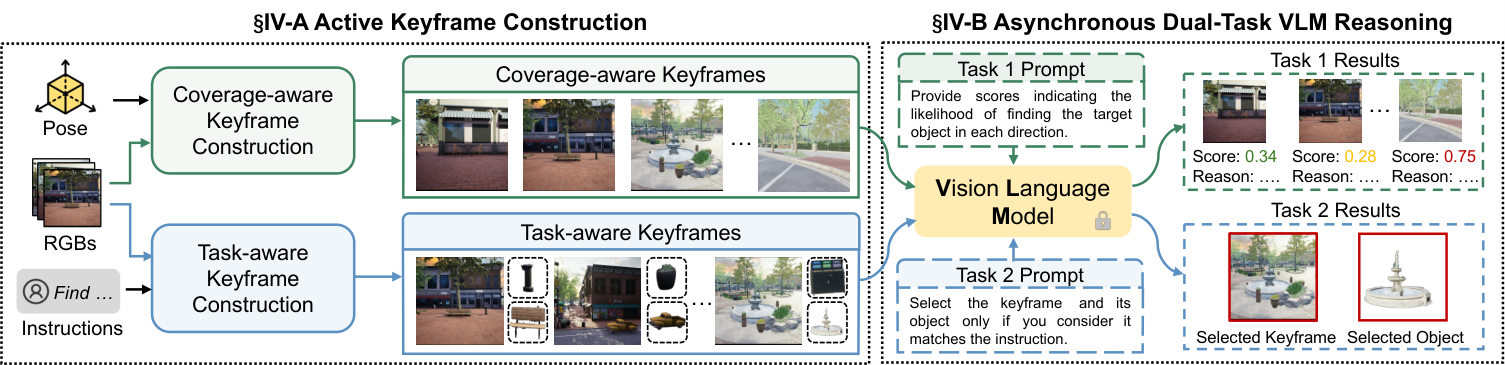
\includegraphics[width=\linewidth,height=27mm,keepaspectratio]{figures/p_airhunt_keyframes.png}\par{\fontsize{6.6}{8}\selectfont\color{muted}AirHunt · Figure 3（论文原图）}\par\endgroup\vspace{1mm}
\end{minipage}\hfill
\begin{minipage}[t]{0.49\linewidth}\vspace{0pt}\raggedright \par\begingroup\centering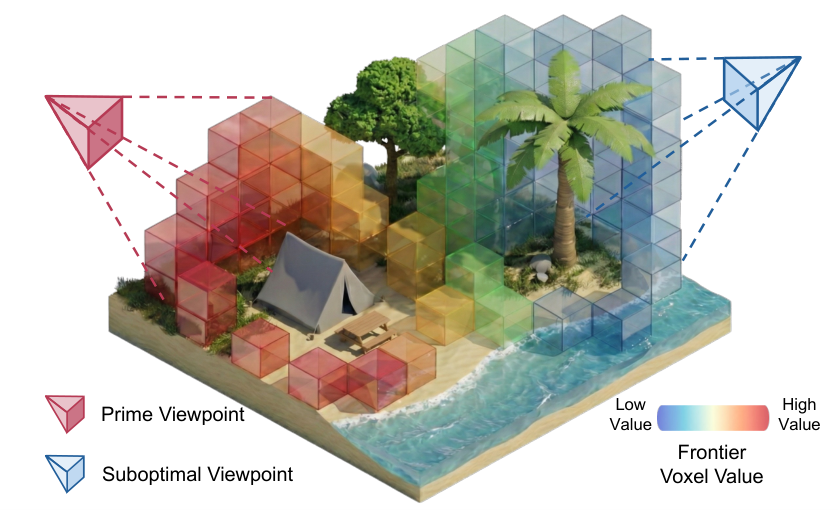
\includegraphics[width=\linewidth,height=27mm,keepaspectratio]{figures/p_airhunt_viewpoints.png}\par{\fontsize{6.6}{8}\selectfont\color{muted}AirHunt · Figure 4（论文原图）}\par\endgroup\vspace{1mm}
\end{minipage}\par
{\fontsize{8.0}{10.1}\selectfont
\rowcolors{2}{white}{zebra}
\begin{tabularx}{\linewidth}{@{}Y{0.78}Z{0.54}Y{1.68}@{}}\toprule
\rowcolor{navy}\thd{同协议配置} & \thd{SR（\%）} & \thd{变化来自哪里}\\\midrule
完整／最近帧 & 73.1 ／ 59.3 & 覆盖帧加目标帧，比只看最近帧多14个点\\
RecTask2 & 31.2 & 保留确认，改用原图直接判断可见性与距离\\
语义贪心 & 16.2 & 去掉全局访问优化，只按语义值贪心\\
\bottomrule\end{tabularx}\par}
\takeaway{关键帧提高语义信号质量，几何核验提高实例判断，全局访问优化抑制多个高值区域之间的往返。}

\note{覆盖关键帧按体素视域重叠筛选，使VLM在有限调用内保留较广的区域语义；任务关键帧保留有候选目标的局部细节。语义前沿同时按空间接近与语义相似性聚类，候选视点聚合可见前沿的语义价值。全局规划给高价值区域注入选择性的访问优先约束，保留几何旅行优化的自由度，局部轨迹持续根据实测地图更新。最近帧59.3、原图直接判断目标可见性与距离31.2、语义贪心16.2，与完整73.1共同说明三层机制各有作用。}
\end{frame}
\gdef\slidesource{原文依据：\href{https://arxiv.org/html/2602.00551v1}{[9] APEX}}
\begin{frame}[t,label=apex]{APEX：持久三维图与独立grounding}
\relax

\noindent\begin{minipage}[t]{0.58\linewidth}\vspace{0pt}\raggedright \par\begingroup\centering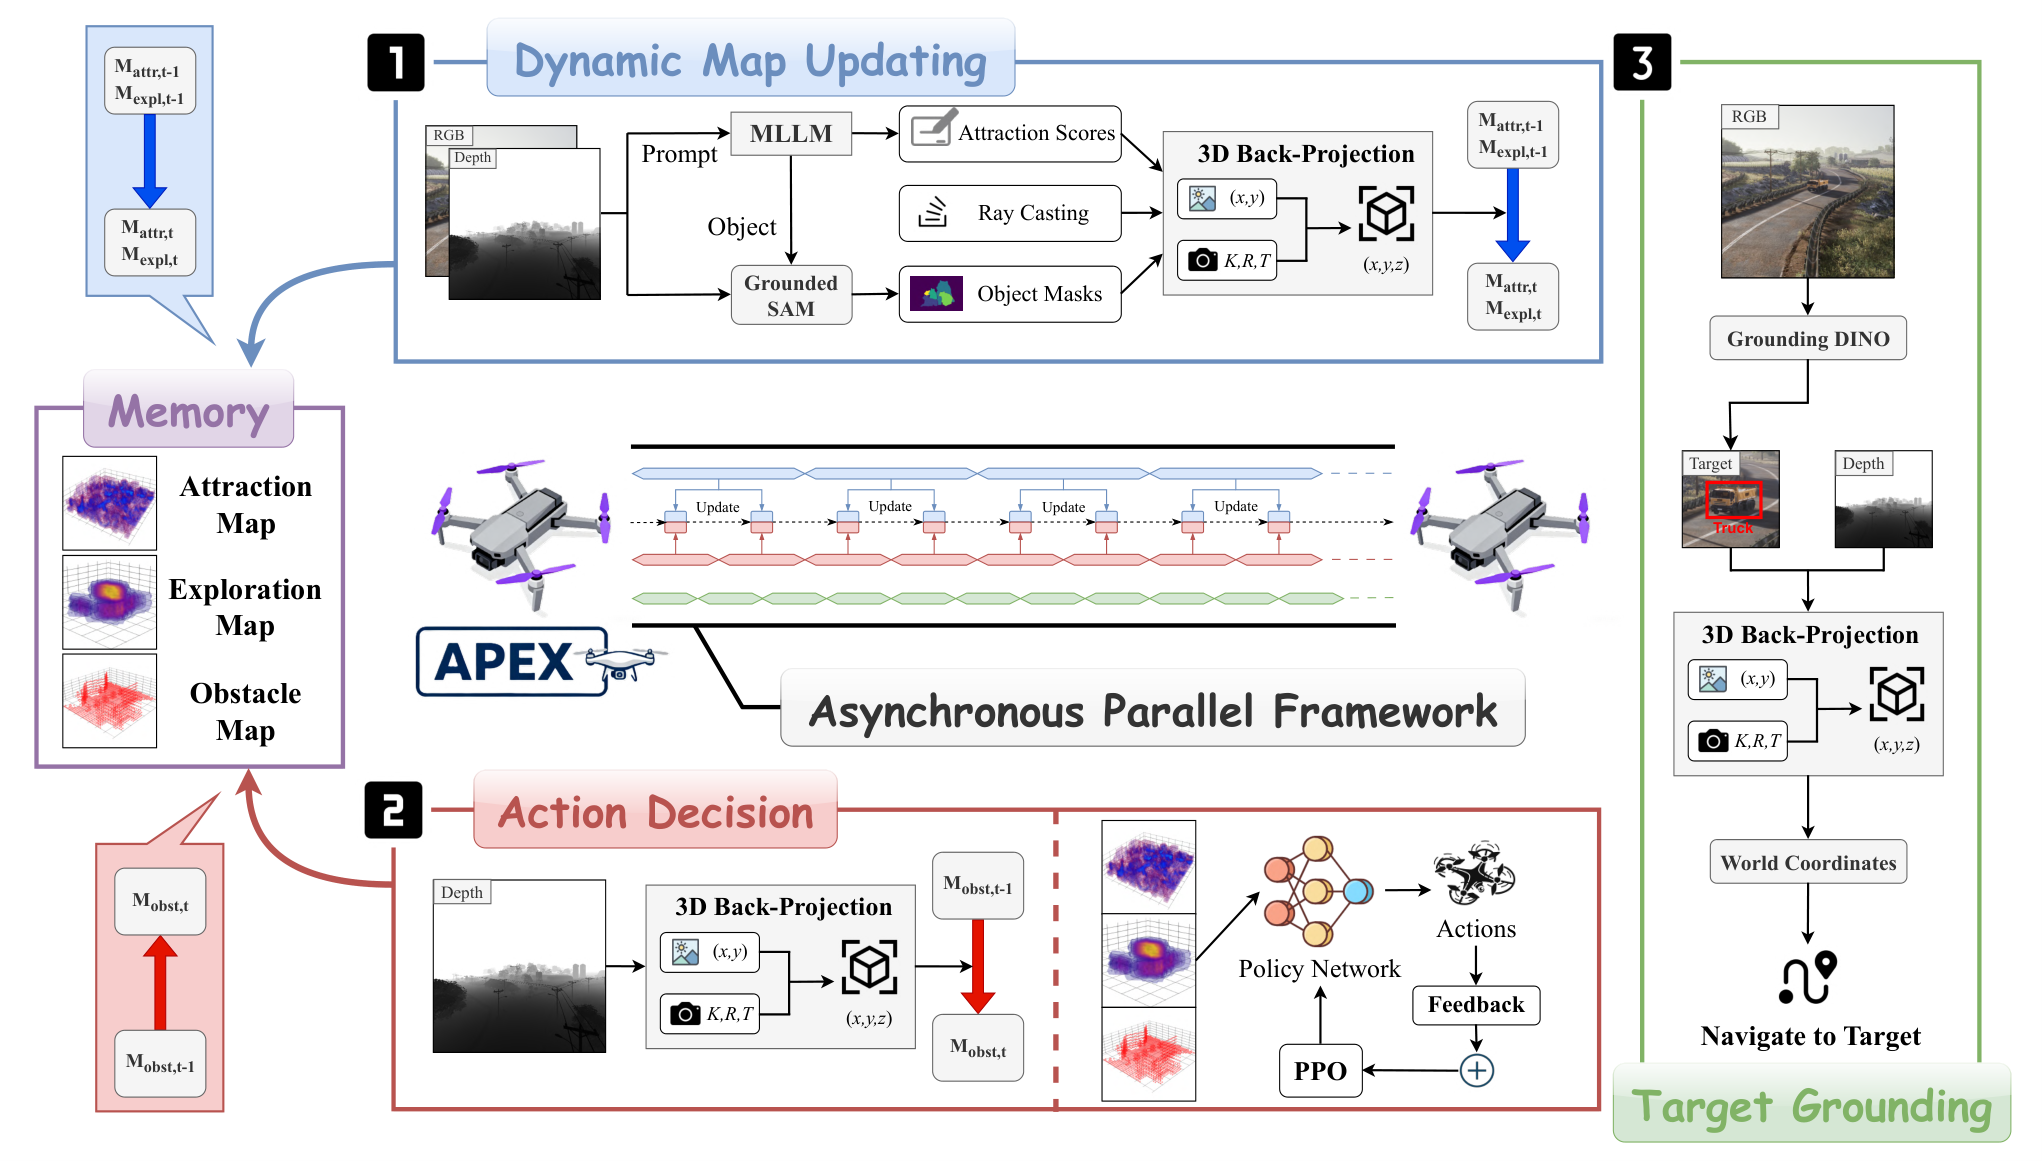
\includegraphics[width=\linewidth,height=36.5mm,keepaspectratio]{figures/p_apex.png}\par{\fontsize{6.6}{8}\selectfont\color{muted}APEX · Figure 2（论文原图）}\par\endgroup\vspace{1mm}
\end{minipage}\hfill
\begin{minipage}[t]{0.4\linewidth}\vspace{0pt}\raggedright {\fontsize{8.9}{11.0}\selectfont\par\ph{模块与训练}\quad 三张三维图（吸引、探索、障碍）经CNN融合，PPO输出离散动作；grounding独立线程持续跑，架构允许异步。\par\vspace{0.6mm}
\par\ph{训练条件}\quad 9环境\ensuremath{\times}4任务=36，4并行环境、每任务10回合；两阶段PPO（先纯探索，再加吸引／成功奖励）。\par\vspace{0.6mm}
\par\ph{消融怎么读}\quad 无RL与完整只差0.83点，无3D图掉到1.67；主因是地图和grounding。三维记忆和终端grounding贡献最大。\par\vspace{0.6mm}}
\end{minipage}\par
{\fontsize{8.0}{10.1}\selectfont
\rowcolors{2}{white}{zebra}
\begin{tabularx}{\linewidth}{@{}Y{1.0}Z{1.0}Z{1.0}Z{1.0}Z{1.0}@{}}\toprule
\rowcolor{navy}\thd{同篇消融} & \thd{完整} & \thd{无RL} & \thd{替换TG} & \thd{无3D图}\\\midrule
SR /\allowbreak{} SPL（\%） & 13.33 /\allowbreak{} 10.14 & 12.50 /\allowbreak{} 10.11 & 5.00 /\allowbreak{} 4.17 & 1.67 /\allowbreak{} 0.73\\
\bottomrule\end{tabularx}\par}
\takeaway{三张地图分别提供目标吸引、已观测密度与障碍约束；独立grounding将区域探索切换为目标接近。}

\note{吸引图先让MLLM输出对象及与目标的相关分数，分割后反投影到世界体素；每个体素由投影像素最多的对象占有，并优先更新更近的观测。探索图用深度射线累计观测密度，障碍图快速更新碰撞占据。CNN融合地图与自身状态，PPO学习离散运动；独立Grounding DINO线程发现目标后触发接近。训练先纯探索再引入目标吸引与成功奖励，语义地图可离线预计算；部署时在线更新语义。整体SR13.33，无RL12.50，无地图1.67，替换grounding5.00，说明持久地图和最后阶段的目标定位是主要贡献。}
\end{frame}
\gdef\slidesource{原文依据：\href{https://arxiv.org/html/2606.14772v1}{[12] ScoutVLA}}
\begin{frame}[t,label=scout]{ScoutVLA：取景与回答共享上下文}
\relax
\par\begingroup\centering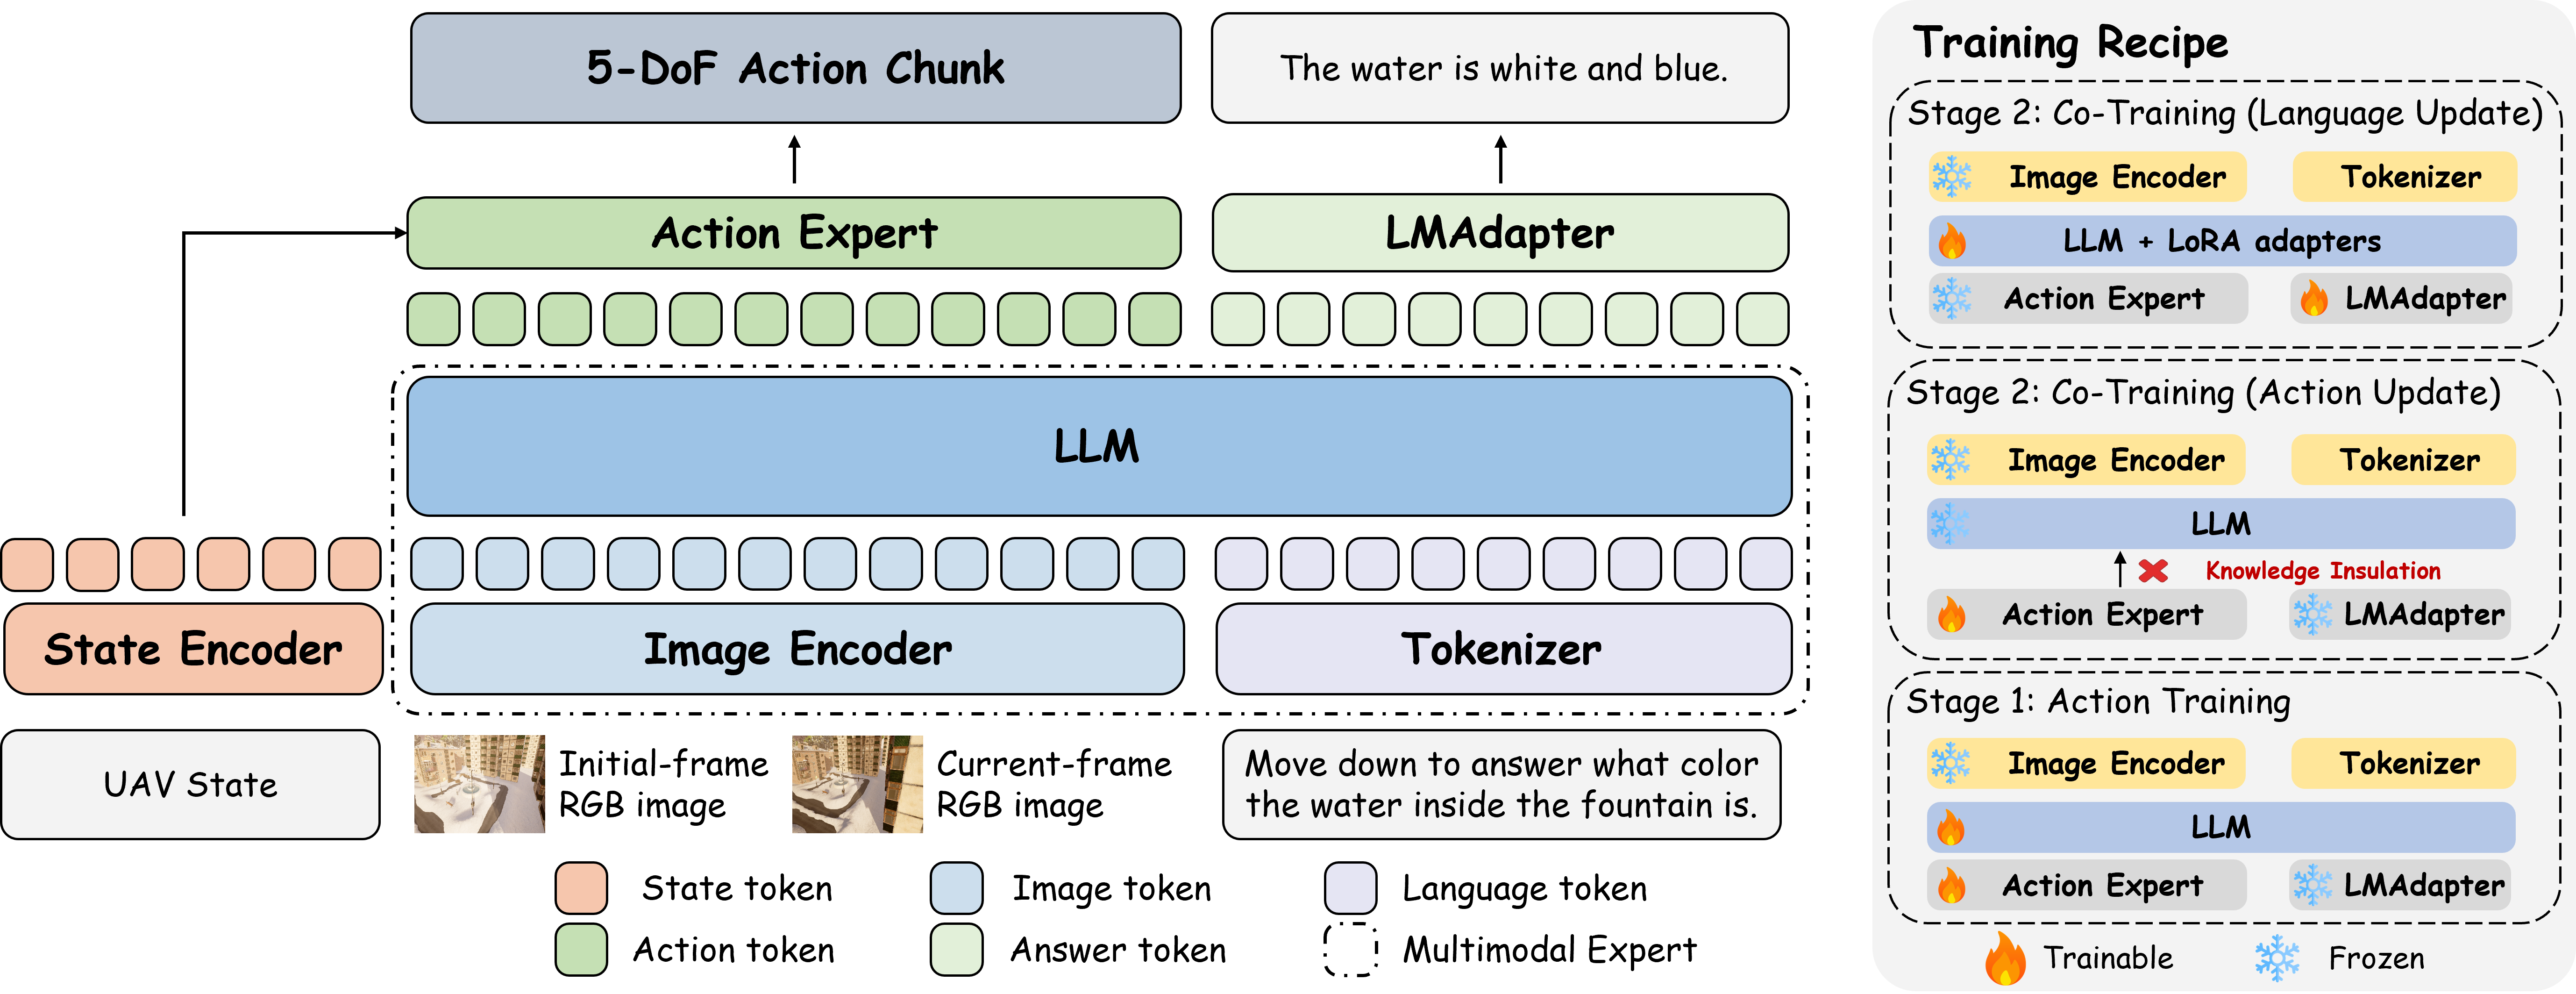
\includegraphics[width=\linewidth,height=30.0mm,keepaspectratio]{figures/p_scout.png}\par{\fontsize{6.6}{8}\selectfont\color{muted}ScoutVLA · Figure 2（论文原图）}\par\endgroup\vspace{1mm}

\noindent\begin{minipage}[t]{0.3233333333333333\linewidth}\vspace{0pt}\raggedright \par\ph{输入与动作}\quad 当前／初始图像、问题和状态；动作专家输出平移、yaw、云台pitch和STOP，五自由度用七个网络通道编码。\par\vspace{1mm}
\end{minipage}\hfill
\begin{minipage}[t]{0.3233333333333333\linewidth}\vspace{0pt}\raggedright \par\ph{训练分工}\quad PaliGemma 2双专家；第二阶段冻结语义主干，动作批与QA批按3:1交替；动作网络、LoRA、语言适配器分别更新。\par\vspace{1mm}
\end{minipage}\hfill
\begin{minipage}[t]{0.3233333333333333\linewidth}\vspace{0pt}\raggedright \par\ph{推理与结果}\quad 先取景，停止后生成短答案。TDR/\allowbreak{}QAC/\allowbreak{}SSR=80.99/\allowbreak{}72.70/\allowbreak{}71.90\%，三个指标测的不是同一个事件。\par\vspace{1mm}
\end{minipage}\par
\takeaway{架构核心：用问题语义条件化机体与云台控制，再在取得的终端视图上生成短答案。}

\note{PaliGemma 2多模态专家提供图像和问题上下文，flow matching动作专家生成五自由度视角调整。动作编码含三维平移、yaw与云台pitch以及停止相关通道。第一阶段以动作去噪学习视觉到控制映射，第二阶段冻结语义主干并加入LoRA和LMAdapter，按3:1交替动作与语言批次，以知识隔离约束梯度更新范围。移除LoRA几乎不改变TDR却让QAC降到12.32，说明飞到合适位置与领域问答能力都需要训练。}
\end{frame}
\gdef\slidesource{原文依据：\href{https://arxiv.org/html/2606.14772v1}{[12] ScoutVLA}}
\begin{frame}[t,label=scout_data]{ScoutVLA：专家终端视图如何形成监督}
\relax

\noindent\begin{minipage}[t]{0.54\linewidth}\vspace{0pt}\raggedright \par\begingroup\centering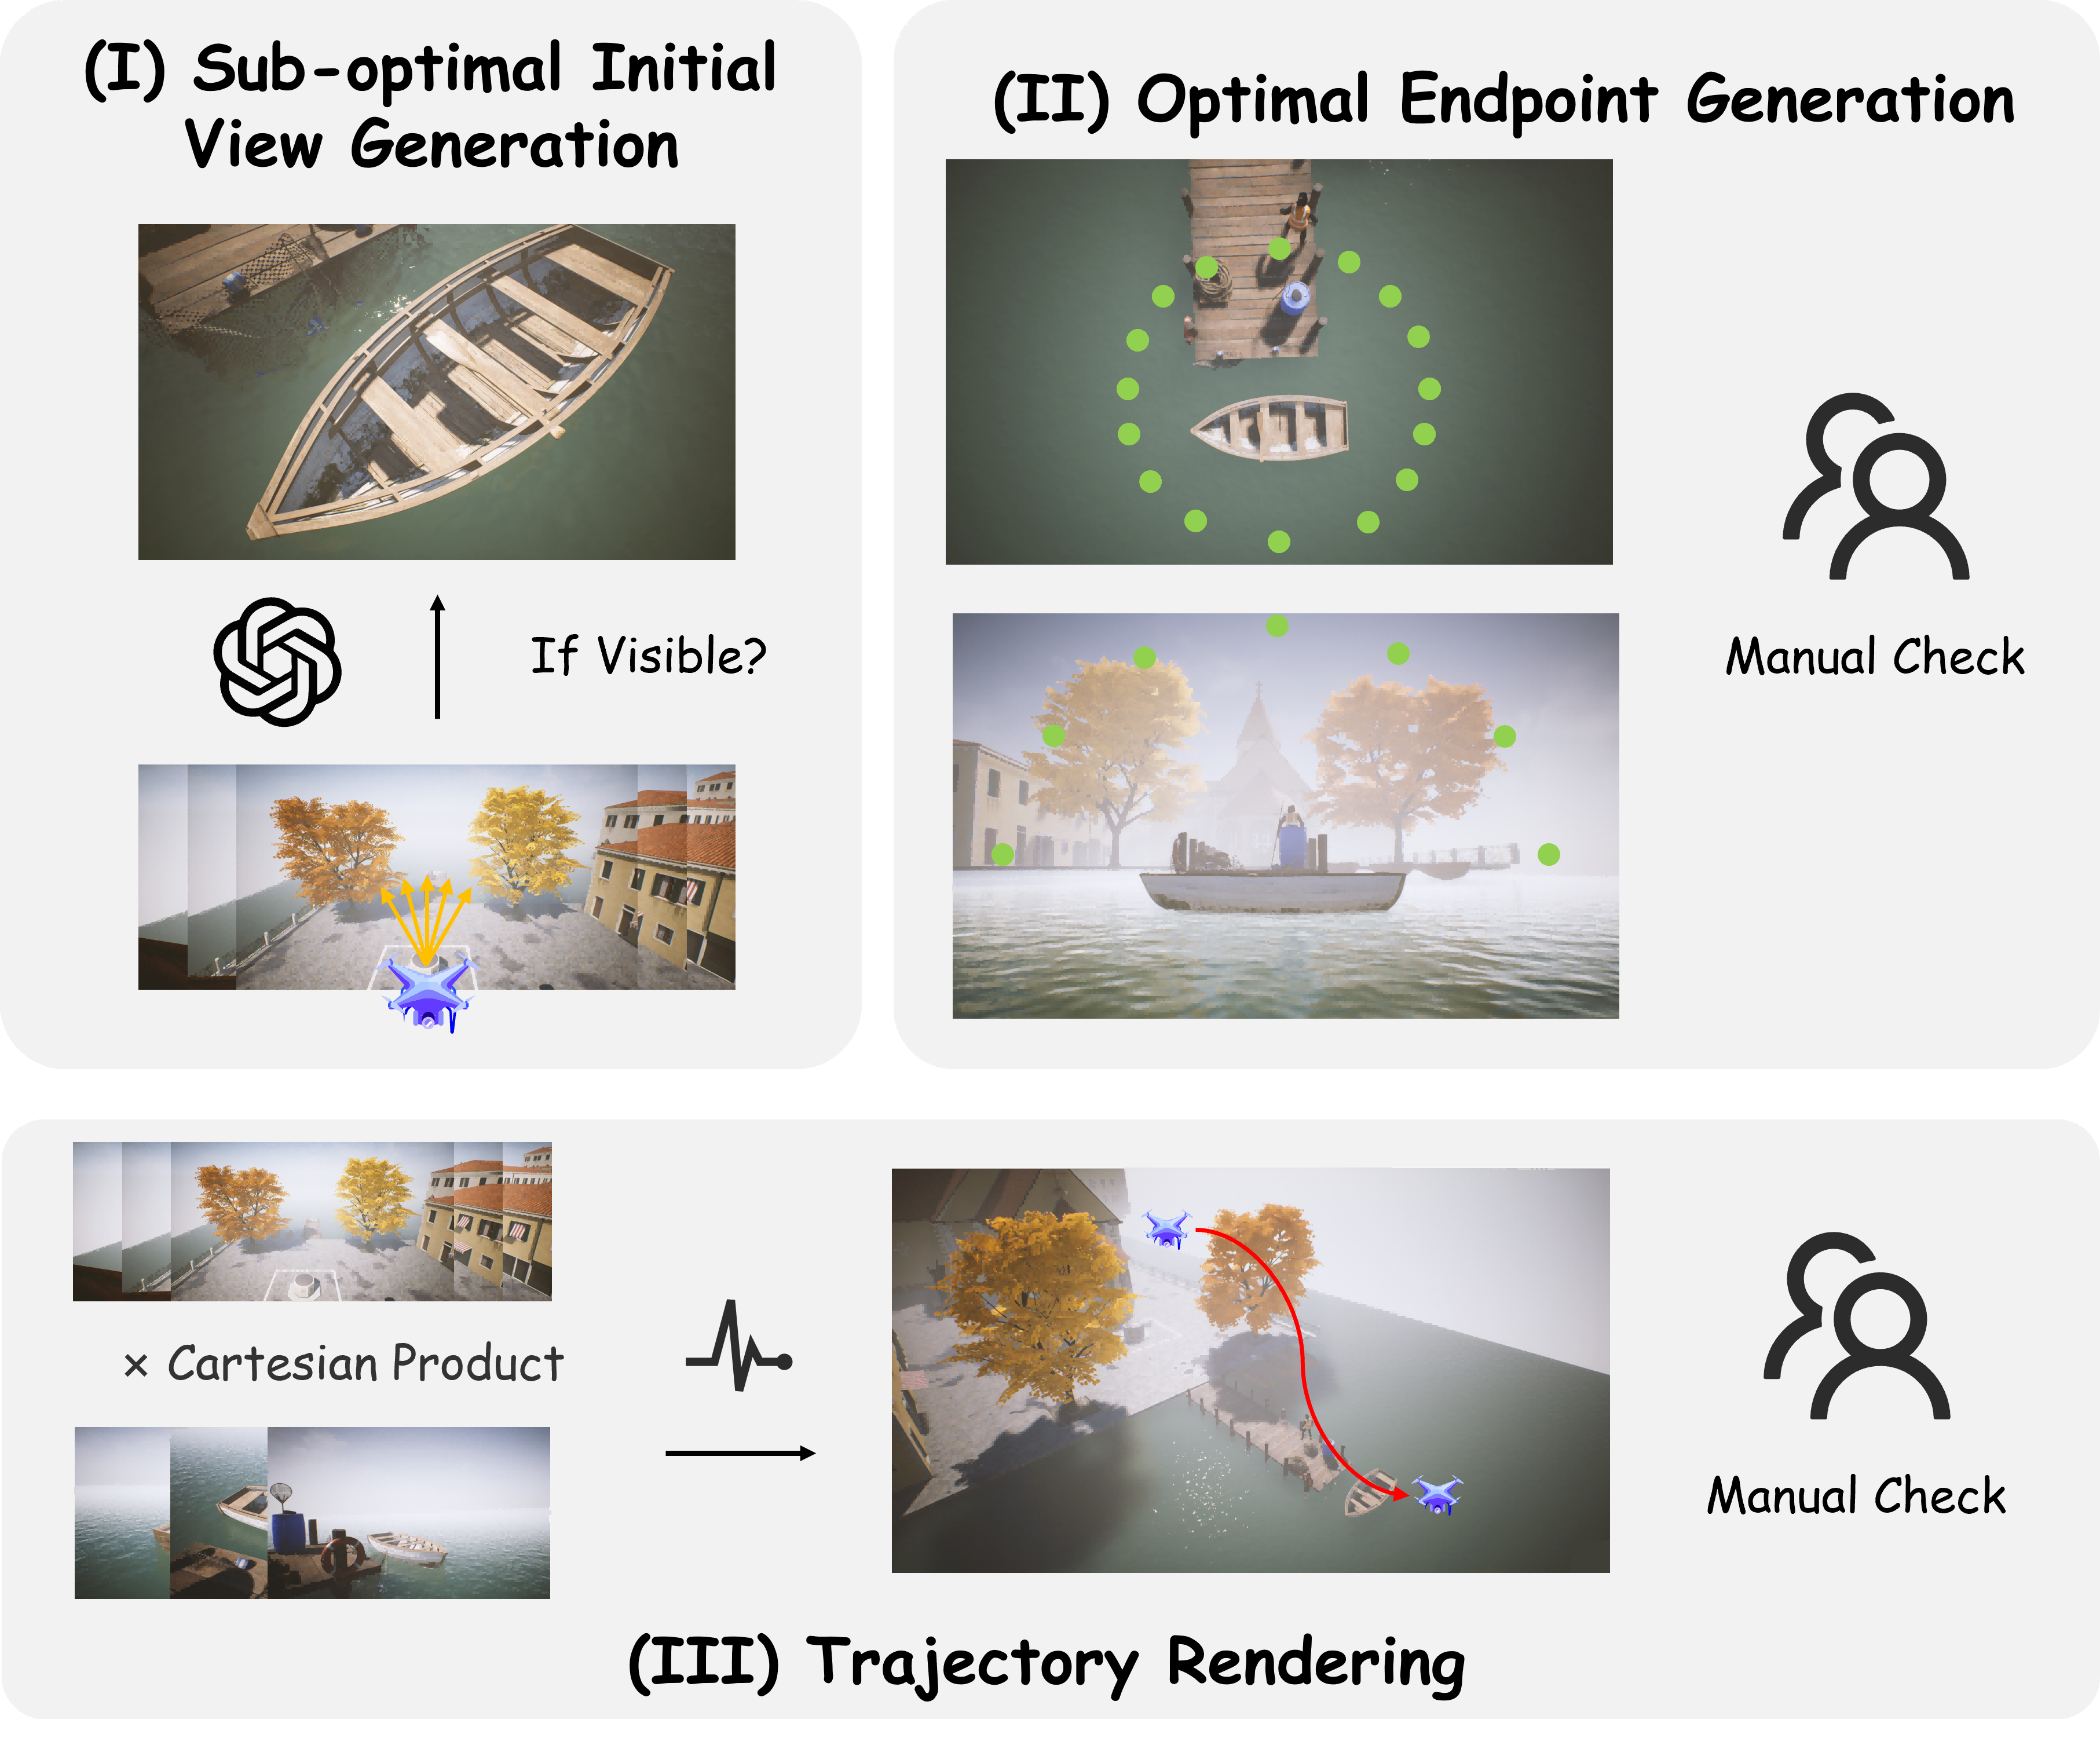
\includegraphics[width=\linewidth,height=36mm,keepaspectratio,trim=0.000bp 250.039bp 0.000bp 0.000bp,clip]{figures/p_scout_pipeline.png}\par{\fontsize{6.6}{8}\selectfont\color{muted}ScoutVLA · Figure 4（原图局部放大）}\par\endgroup\vspace{.5mm}
\end{minipage}\hfill
\begin{minipage}[t]{0.44\linewidth}\vspace{0pt}\raggedright \par\ph{监督怎么来}\quad 40K仿真＋1K真实轨迹；从目标可见起点，在上半球采候选，由专家选可回答终点并生成轨迹。\par\vspace{.5mm}
\par\ph{恢复样本}\quad 30\%轨迹加入姿态扰动，补偏移后的视角恢复。\par\vspace{.5mm}
\par\ph{实验分解}\quad 表3固定外部VQA：Pi05终端视图QAC 36.27，Pi0为34.43；通用VLM终端视图为3.96–9.30。\par\vspace{.5mm}
\par\ph{另一能力}\quad 表4独立VQA为95.40；去掉LoRA后TDR 80.85、QAC 12.32，回答适配同样关键。\par\vspace{.5mm}
\end{minipage}\par
\takeaway{固定外部回答器后，ScoutVLA取得的视图仍更容易回答问题；收益同时来自取景学习与领域问答适配。}

\note{FG-EQA包含40K仿真与1K真实轨迹，从目标可见或部分可见的初始视角出发，在上半球采样终端候选并由专家筛选可回答位置。30\%轨迹增加姿态扰动以学习恢复。Table3将不同策略的终端FPV图固定后交给同一外部VQA模型面板，Pi05终端视图平均QAC36.27，Pi0为34.43，通用VLM策略的终端视图为3.96–9.30。Table4则在留出的无人机VQA样本上测试回答模型，Pi05达到95.40。两组实验分别支持视图获取和回答能力的贡献。}
\end{frame}
\gdef\slidesource{\href{https://arxiv.org/html/2607.10180v2}{[13] ActiveFly-Bench} · §3–5；Figs.1–3}
\begin{frame}[t,label=activefly_arch]{ActiveFly：观察计划、五自由度执行与历史问答}
\relax
\par\begingroup\centering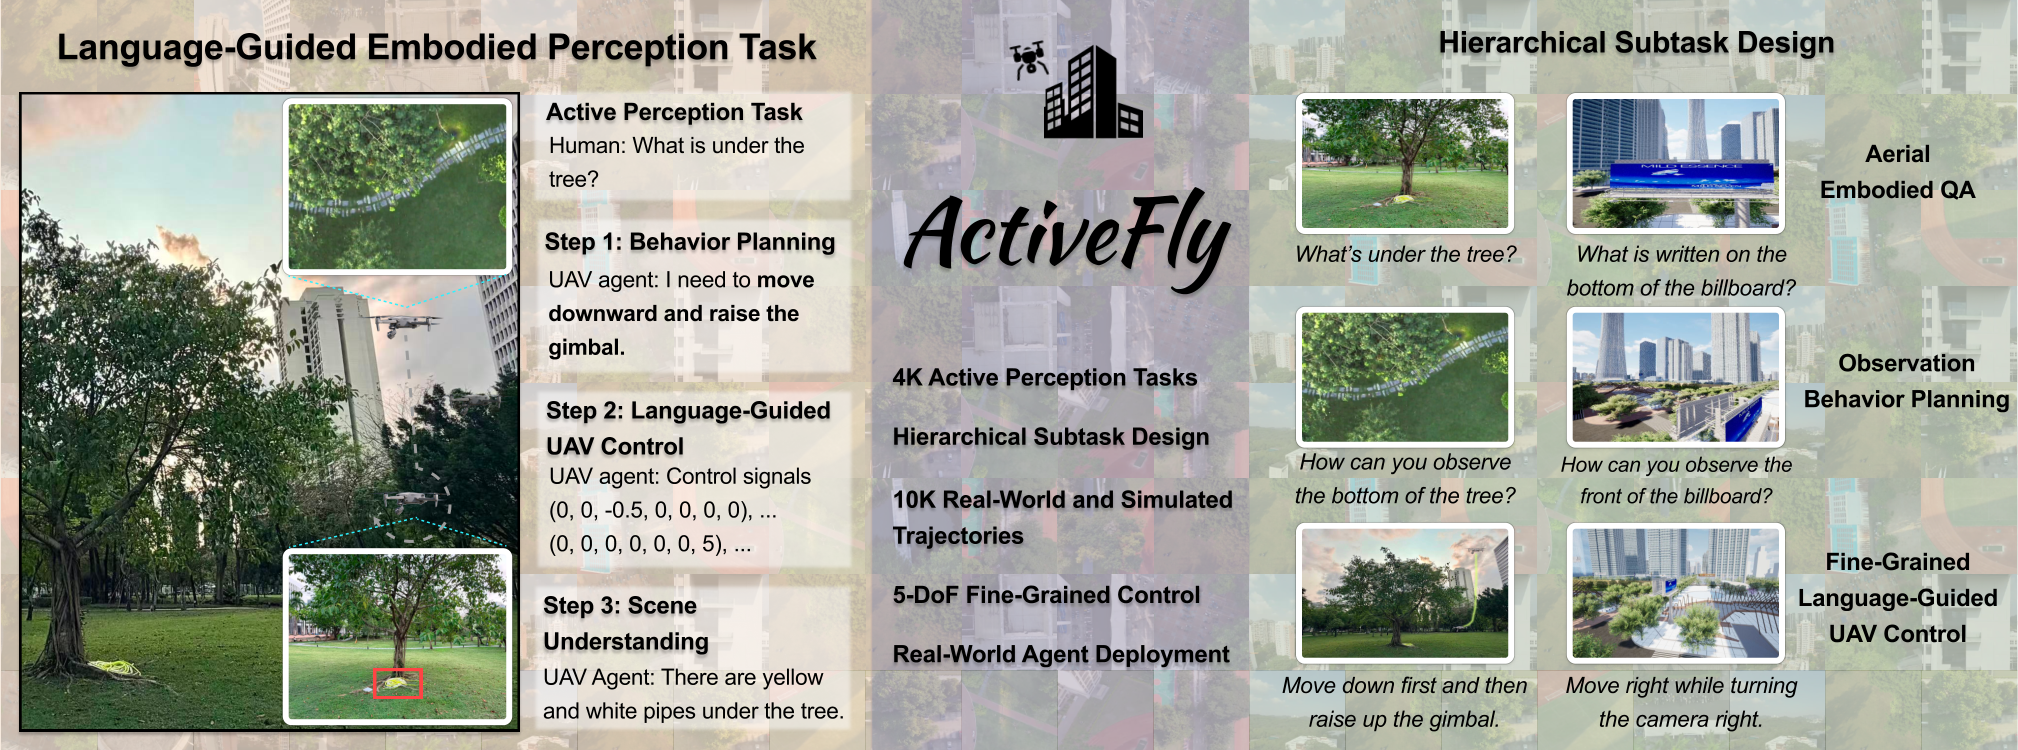
\includegraphics[width=\linewidth,height=28mm,keepaspectratio]{figures/p_activefly.png}\par{\fontsize{6.6}{8}\selectfont\color{muted}ActiveFly-Bench Fig.1：Air-EQA、OBP与FLUC三级任务}\par\endgroup\vspace{1mm}

\noindent\begin{minipage}[t]{.323\linewidth}\vspace{0pt}\raggedright \ph{高层观察规划}\quad VLM根据初始图与问题生成文字观察行为，如绕到正面、接近标牌、抬云台；OBP检验问题到观察意图的转换。\par\end{minipage}\hfill\begin{minipage}[t]{.323\linewidth}\vspace{0pt}\raggedright \ph{低层执行与回答}\quad VLA将观察描述、当前图像及状态变为平移、yaw和云台pitch；执行后从历史采16帧，由VLM汇总回答。\par\end{minipage}\hfill\begin{minipage}[t]{.323\linewidth}\vspace{0pt}\raggedright \ph{数据与诊断}\quad 10K轨迹，含10种基本与4种复杂观察行为，覆盖遮挡、非正面、视野边缘及远距模糊；三级独立评价定位误差来源。\par\end{minipage}
\takeaway{方法要点：文字观察行为把“要获取什么信息”与“怎样调整机体和云台”连接起来。}
\note{ActiveFly采用分层系统而非一体双专家。问题与初始观察先送VLM产生观察行为描述；VLA依据该描述执行连续五自由度运动；停止后VLM读16帧历史给答案。数据从真实校园、真实室内以及两个高保真城市环境采集，初始图存在至少一种观察限制，终端图应能看清目标。部署时VLM和VLA运行在RTX A6000地面服务器，机载运行SLAM与路径规划，采用stop-and-infer等待策略。该分解允许单独替换高层、执行器和问答模型，对系统瓶颈进行定位。}
\end{frame}
\gdef\slidesource{原文依据：\href{https://arxiv.org/html/2607.10180v2}{[13] ActiveFly}；\href{https://arxiv.org/html/2606.14772v1}{[12] ScoutVLA}}
\begin{frame}[t,label=activefly]{ActiveFly实验：观察计划正确仍受执行与问答约束}
\relax
{\fontsize{8.7}{11.1}\selectfont
\rowcolors{2}{white}{zebra}
\begin{tabularx}{\linewidth}{@{}Y{0.69}Y{1.29}Y{1.02}@{}}\toprule
\rowcolor{navy}\thd{配置（每行独立）} & \thd{论文报告（\%）} & \thd{说明}\\\midrule
GPT-5.4＋\ensuremath{\pi}0.5 & FLUC SR 31，OSR 71；EP 47.8 & 能到目标附近，停止和答题拖后腿\\
Gemini＋\ensuremath{\pi}0.5 & EP 49.4 & 换高层模型，低层仍是同一个\ensuremath{\pi}0.5\\
Human＋\ensuremath{\pi}0.5 & EP 60.3 & 高层对了，执行与答题仍损失约四成\\
Human Agent & EP 97.3 & 完整人类上界，用来定位瓶颈\\
\bottomrule\end{tabularx}\par}
\[S_{\rm EP}=S_{\rm OBP}\;OS_{\rm FLUC}\;S_{\rm EQA}\]\par\ph{时延构成}\quad 390ms不含高层规划与QA，120ms是传输开销；整机闭环要把这几段相加。\par\vspace{1mm}
\par\ph{实验范式}\quad 固定回答器、观察计划、执行器中的两个，只换一个，比较新视图是否改变任务判定。\par\vspace{1mm}
\takeaway{Human＋\ensuremath{\pi}0.5达到60.3，完整Human为97.3：高层计划和低层执行需要协同改进。}

\note{表2的EP是闭环感知综合指标，FLUC与Air-EQA分别测低层执行和问答。GPT-5.4＋\ensuremath{\pi}0.5的FLUC SR31、OSR71，说明到过适合区域而未正确结束是重要损失；EP为47.8。把高层换成人类后EP60.3，完整人类97.3，显示仅提高高层规划不能消除执行和问答误差。不同模型行保持各自配置，公式表示各环节组合关系。390ms指VLA相关时延，端到端还包括高层规划、通信和最终回答。}
\end{frame}
\gdef\slidesource{原文依据：\href{https://arxiv.org/html/2601.07558v1}{[14] FlyCo}}
\begin{frame}[t,label=flyco]{FlyCo：预测未见表面，执行后补实测}
\relax

\noindent\begin{minipage}[t]{0.57\linewidth}\vspace{0pt}\raggedright \par\begingroup\centering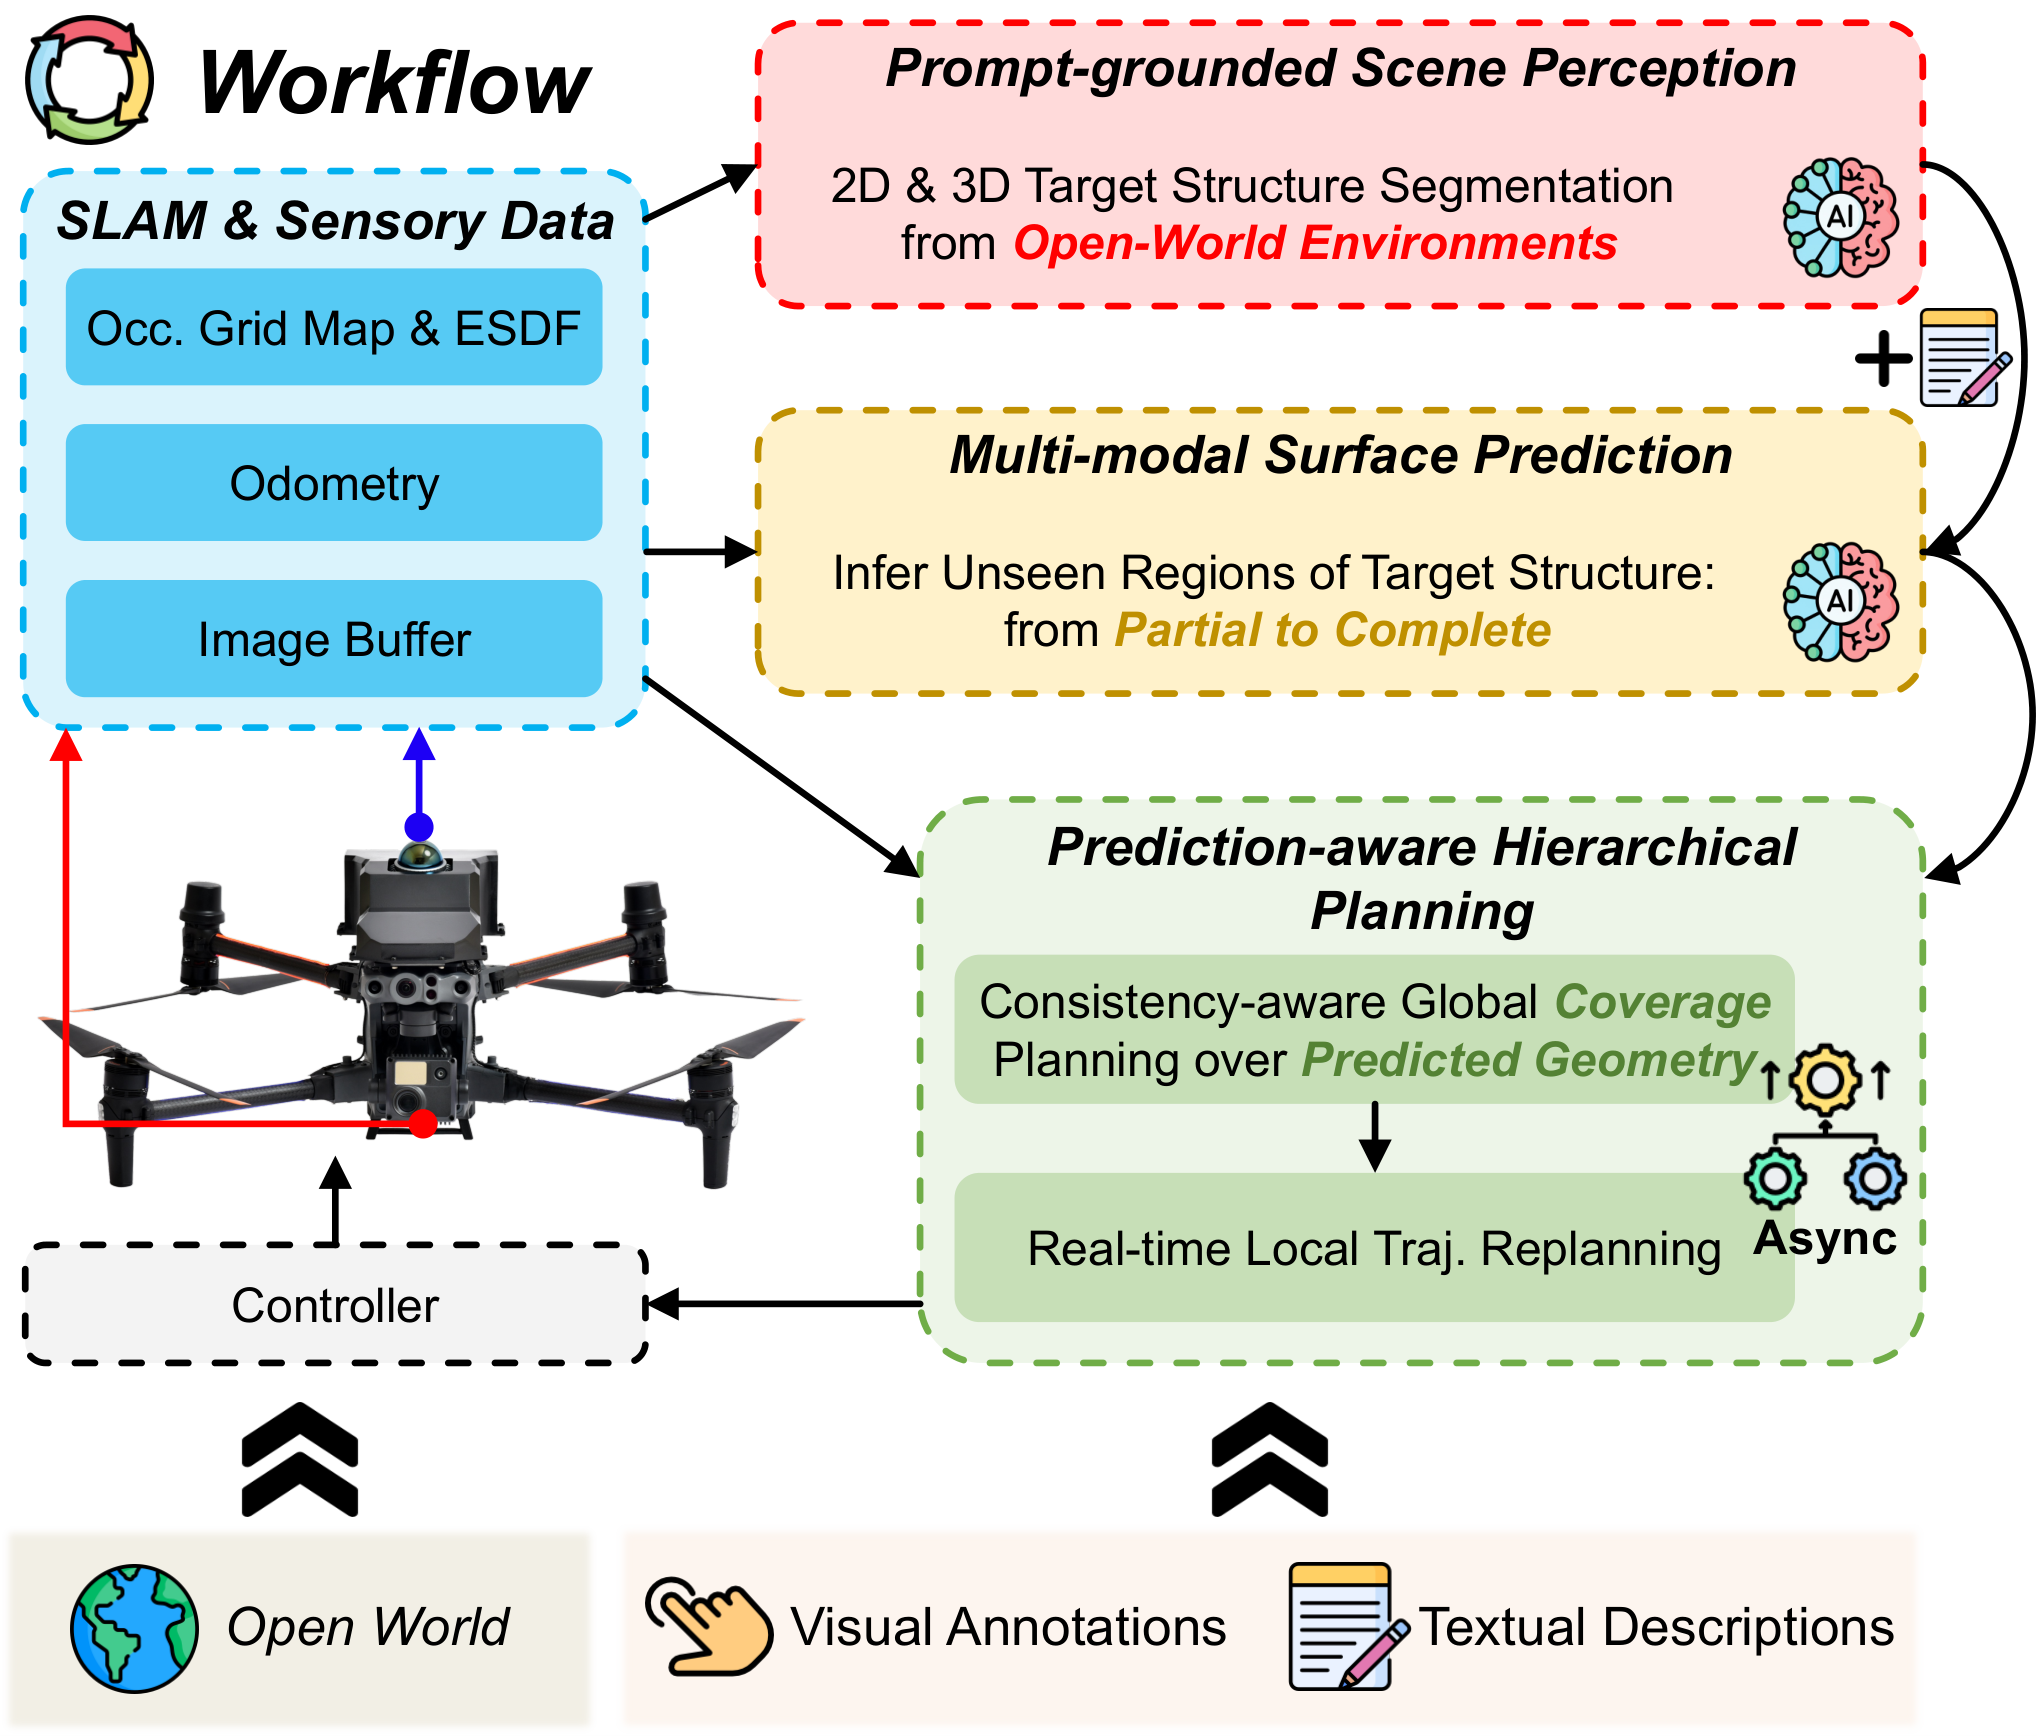
\includegraphics[width=\linewidth,height=48mm,keepaspectratio]{figures/p_flyco.png}\par{\fontsize{6.6}{8}\selectfont\color{muted}FlyCo · Figure 3（论文原图）}\par\endgroup\vspace{1mm}
\end{minipage}\hfill
\begin{minipage}[t]{0.41\linewidth}\vspace{0pt}\raggedright \par\ph{启动与表征}\quad 文本加一张起始图像的一次粗2D标注；RGB-LiDAR观测结合多模态表面预测，初始化目标的2D／3D对应。\par\vspace{1mm}
\par\ph{闭环规划}\quad 预测几何用来选全局覆盖视点，实测地图和当前状态管局部轨迹；预测与实测分开存。\par\vspace{1mm}
\par\ph{数据与效果}\quad 7万个结构资产训练预测器；4类结构各20次，完整性93.83–96.50\%，完成79/\allowbreak{}80。\par\vspace{1mm}
\par\ph{计算与尺度}\quad 以0.05m体素统计表面完整性；感知、预测、全局覆盖与局部规划异步运行。\par\vspace{1mm}
\end{minipage}\par
\takeaway{核心闭环：用预测完整结构规划尚未观察的表面，再由新实测持续修正结构与覆盖路线。}

\note{FlyCo从人类给定的文本及一次稀疏2D提示初始化目标。感知模块用视觉分割和LiDAR几何双向校正，预测模块融合点云、图像、相机参数和文本补全结构，规划模块对未观测表面生成覆盖视点，并保持多轮路径一致性。实测地图承担局部避障，新增扫描持续更新目标几何。完整性采用体素表面覆盖统计，79/80为四种结构各20次试验的完成数量。}
\end{frame}
\gdef\slidesource{\href{https://arxiv.org/html/2601.07558v1}{[14] FlyCo} · §5.2–5.3；Fig.4、7；§6}
\begin{frame}[t,label=flyco_predict]{FlyCo：多模态形状补全与一致性覆盖规划}
\relax
\bline{几何、图像与文本融合}{目标点云用FPS下采样，选择与3D目标最一致的图像；DINO图像特征、文本和点云特征投影至共同空间，经交替注意力补全结构。}
\bline{训练约束}{约7万结构资产产生多模态样本；partial与completion Chamfer损失分别保持已见表面一致并恢复完整形状，推理后再做几何增密。}
\bline{全局覆盖}{对预测网格中未观察表面选少量覆盖视点，再优化访问次序；引入历史路径一致性，抑制每次补全更新引起的路线反转。}
\bline{局部执行}{从全局路径截取有限时域片段，用最新占据／ESDF地图和A*修正，再优化平滑、动态可行且满足观察方向的轨迹。}\takeaway{预测的作用是提前组织覆盖，实测的作用是更新真实表面与局部障碍；两者通过分层规划形成闭环。}
\note{FlyCo的预测器以归一化的局部点云、带相机参数的目标图像和文本为输入，输出补全点集。10层交替注意力在几何与语义之间融合；partial与completion Chamfer损失强调观测忠实度与完整性。感知侧采用固定窗口SAM2，并用LiDAR目标点云重投影检查分割一致性：不一致时从3D目标采样虚拟提示点重启2D分割。规划侧在视点生成和路径次序两阶段都维持时间一致性，兼顾更新效率；局部地图决定即时避障。4类结构80次试验79次完成，表面完整性93.83–96.50\%。}
\end{frame}
\section{世界动作模型}
\gdef\slidesource{原文依据：\href{https://arxiv.org/html/2512.21887v2}{[15] ANWM}；\href{https://arxiv.org/html/2609.33581v1}{[18] ForeFly}；\href{https://arxiv.org/html/2605.15964v1}{[16] WorldVLN}；\href{https://arxiv.org/html/2609.39763v1}{[20] DiffWAM}}
\begin{frame}[t,label=wam_interfaces]{世界动作模型的六种预测与解码接口}
\relax
{\fontsize{8.7}{11.1}\selectfont
\rowcolors{2}{white}{zebra}
\begin{tabularx}{\linewidth}{@{}Y{0.6}Y{1.08}Y{1.12}Y{1.2}@{}}\toprule
\rowcolor{navy}\thd{方法} & \thd{预测什么} & \thd{动作接口} & \thd{群体能拿它做什么}\\\midrule
ANWM & 动作条件未来视图 & 五个候选，末端LPIPS选路 & 在给定候选里评后果\\
ForeFly & 下一步／关键事件特征 & attention＋FiLM细化方向和步长 & 提供任务条件提案\\
WorldVLN & 自回归世界token & 预测表征后解码动作 & 短片段执行，执行后重锚\\
WorldFly & 未来／动作latent & 双分支flow联合生成 & 策略耦合，不直接给信息收益\\
ImagineUAV & 生成视频 & VO读运动，动力学规划 & 生成可跟踪的运动参考\\
DiffWAM & 早期DiT表征 & 几何读出米制位姿 & 38个未来位姿参考，本地接轨\\
\bottomrule\end{tabularx}\par}
\takeaway{三条架构路线：动作条件未来评价、任务条件世界／动作联合建模、预测表征的几何运动读出。}

\note{WAM不是唯一架构。ANWM给定候选动作预测后果，比较接近候选评价；ForeFly预测任务特征；WorldVLN和WorldFly连接世界与动作；ImagineUAV和DiffWAM读取几何参考。对群体而言最危险的跳跃，是假定任何WAM都能输入任意候选视角并输出信息收益。任务条件策略不一定有这种反事实接口，需要另行适配预测器或价值模型。}
\end{frame}
\gdef\slidesource{\href{https://arxiv.org/html/2512.21887v2}{[15] ANWM} · §3.3–3.4；Figs.2–3；Table 2}
\begin{frame}[t,label=anwm]{ANWM：用几何投影辅助动作条件未来生成}
\relax
\par\begingroup\centering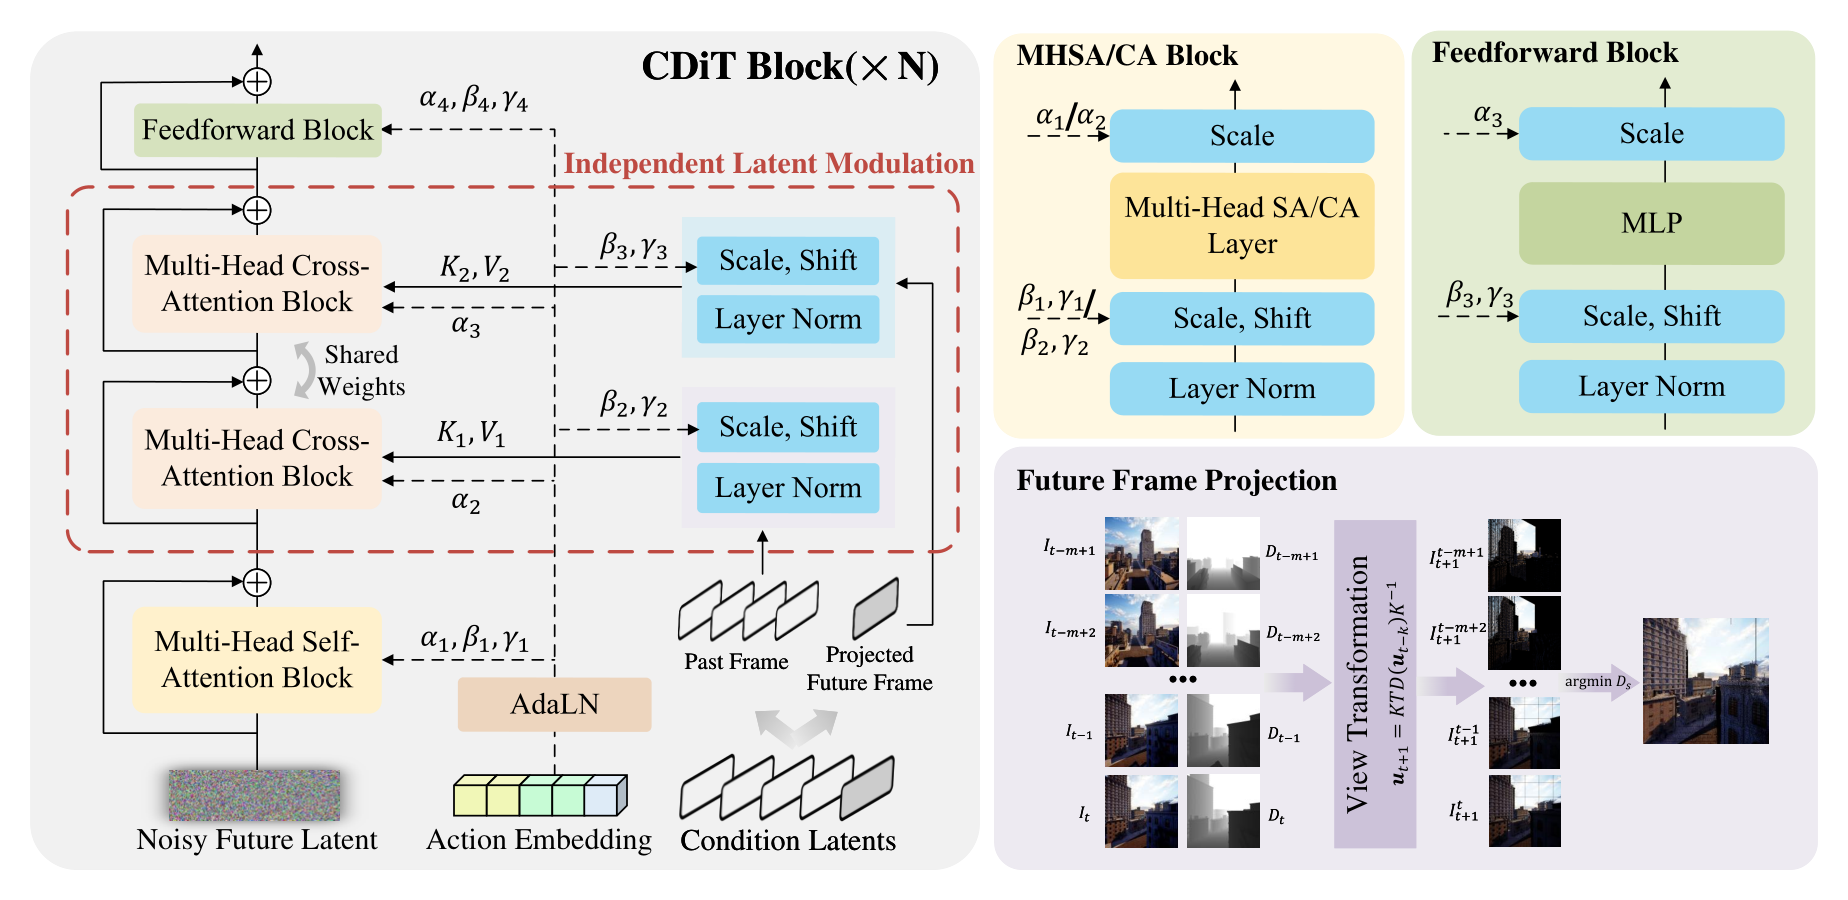
\includegraphics[width=\linewidth,height=28mm,keepaspectratio]{figures/p_anwm.png}\par{\fontsize{6.6}{8}\selectfont\color{muted}ANWM Fig.3：历史帧与投影未来帧的双条件CDiT}\par\endgroup\vspace{1mm}

\noindent\begin{minipage}[t]{.323\linewidth}\vspace{0pt}\raggedright \ph{几何先验}\quad 给定RGB-D历史与候选4D运动，用深度反投影到3D，再变换到未来视角，得到带缺失区域的粗未来图。\par\end{minipage}\hfill\begin{minipage}[t]{.323\linewidth}\vspace{0pt}\raggedright \ph{世界模型}\quad VAE压缩历史／投影图，双条件分支使用独立scale-shift与共享cross-attention；动作正弦编码经AdaLN注入CDiT。\par\end{minipage}\hfill\begin{minipage}[t]{.323\linewidth}\vspace{0pt}\raggedright \ph{导航与结果}\quad 自回归想象5条候选路线，以末端图与目标图的LPIPS选路。100个2D / 3D导航片段SR为73 / 60，NWM为63 / 58。\par\end{minipage}
\takeaway{方法要点：几何投影解释已见区域如何移动，生成模型补未知区域；未来图用于候选路径排序。}
\note{ANWM是图像目标导航：输入当前视觉历史和候选动作，而非直接执行语言指令。数据从现有AVLN轨迹回放，并利用四视角将前进重新解释为横移或后退，得到350K训练片段。Future Frame Projection用历史深度、内参与候选相机变换构成粗未来图，缓解单纯视频生成的跨视角几何漂移。历史与投影条件分别调制后进入共享注意力，动作作为四维相对运动编码。推理从预设动作集采5条路线并加入扰动，逐帧滚动预测，选择目标图LPIPS最低的路线。长距离递归仍有漂移，因此其关键能力是动作后果评价。}
\end{frame}
\gdef\slidesource{\href{https://arxiv.org/html/2606.06147v1}{[17] WorldFly} · §3–5；Fig.1、3；Tables 1–2}
\begin{frame}[t,label=worldfly]{WorldFly：未来视频与动作的双分支耦合生成}
\relax
\par\begingroup\centering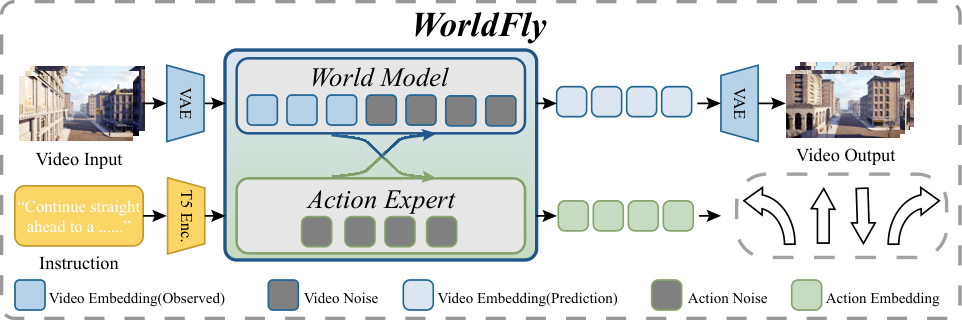
\includegraphics[width=\linewidth,height=28mm,keepaspectratio]{figures/p_worldfly.png}\par{\fontsize{6.6}{8}\selectfont\color{muted}WorldFly Fig.1：双分支coupled flow matching}\par\endgroup\vspace{1mm}

\noindent\begin{minipage}[t]{.323\linewidth}\vspace{0pt}\raggedright \ph{联合建模}\quad T5编码指令，LTX-Video VAE逐帧编码历史。世界分支预测未来latent，动作专家预测动作块，共享同一加噪时刻。\par\end{minipage}\hfill\begin{minipage}[t]{.323\linewidth}\vspace{0pt}\raggedright \ph{耦合机制}\quad 两分支参数独立，间隔插入双向cross-attention；世界特征感知计划动作，动作特征读取预期视觉变化；两种flow损失等权训练。\par\end{minipage}\hfill\begin{minipage}[t]{.323\linewidth}\vspace{0pt}\raggedright \ph{效果与动作接口}\quad 城市路口Easy / Hard SR为87 / 31，去耦合76 / 21；8维连续编码经查表映射为10种飞行原语。\par\end{minipage}
\takeaway{方法要点：在去噪过程中交换世界与动作信息，使两种预测共同对齐同一段未来。}
\note{WorldFly针对低空城市路口大转弯导致的剧烈视角变化构造4K余条路口轨迹。历史latent保持干净，未来视频latent和动作在共享时间上加噪，用两种flow-matching目标恢复。双向耦合层让动作分支利用想象的环境变化，世界分支利用动作约束。动作专家尺寸小于世界模型，采用交叉注意力连接异维特征。实验Easy与Hard各100条，终点阈值12米。删除双分支耦合后SR分别下降11和10个百分点，支持耦合对转弯与未见路口的作用。其8维连续编码是一种动作码，最终执行仍为离散原语。}
\end{frame}
\gdef\slidesource{原文依据：\href{https://arxiv.org/html/2609.33581v1}{[18] ForeFly}}
\begin{frame}[t,label=forefly]{ForeFly：双时域未来在动作中非对称融合}
\relax
\par\begingroup\centering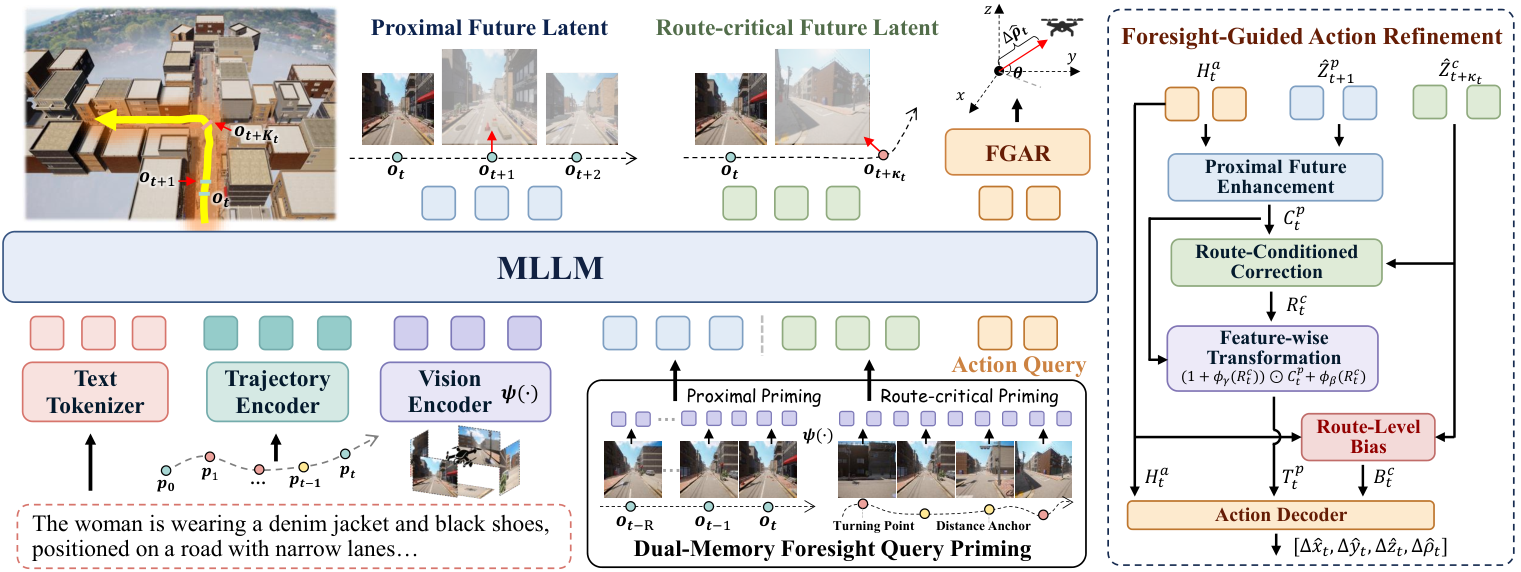
\includegraphics[width=\linewidth,height=26mm,keepaspectratio]{figures/p_forefly.png}\par{\fontsize{6.6}{8}\selectfont\color{muted}ForeFly · Figure 2（论文原图）}\par\endgroup\vspace{1mm}

\noindent\begin{minipage}[t]{0.3233333333333333\linewidth}\vspace{0pt}\raggedright \par\ph{记忆与目标}\quad 当前5个视图，历史只保留前视；近期窗口和转弯／路程锚生成两组各17个查询，远端预测下一个路线关键事件。\par\vspace{0.6mm}
\end{minipage}\hfill
\begin{minipage}[t]{0.3233333333333333\linewidth}\vspace{0pt}\raggedright \par\ph{计算与训练}\quad 动作先读近端未来，再由关键未来做FiLM细化；路线偏置走stop-gradient，主FiLM仍可微。\par\vspace{0.6mm}
\end{minipage}\hfill
\begin{minipage}[t]{0.3233333333333333\linewidth}\vspace{0pt}\raggedright \par\ph{输出与监督}\quad 监督未来特征MSE加方向／步长；输出单位3D方向和步长。未来特征直接服务动作细化，省去RGB重建。\par\vspace{0.6mm}
\end{minipage}\par
\par\ph{实现}\quad LLaMA 2-7B＋EVA-ViT-G，4×RTX 5090；LoRA 5×10$^{-5}$，两阶段训练。\par\vspace{0.3mm}
\takeaway{近端未来提供局部行动线索，关键未来通过FiLM调整这些线索，路线偏置进一步纠正长期方向。}

\note{ForeFly的计算图值得细看：当前5个视图，历史只留前视；近期窗口和转弯／路程锚各生成17个查询。动作网络先读近端未来，再用关键未来做FiLM调制；路线偏置只走stop-gradient，主FiLM仍可微。训练监督是未来特征MSE加方向／步长，在线不生成RGB。}
\end{frame}
\gdef\slidesource{原文依据：\href{https://arxiv.org/html/2609.33581v1}{[18] ForeFly}}
\begin{frame}[t,label=forefly_case]{ForeFly：关键转弯案例与同协议消融}
\relax
\par\begingroup\centering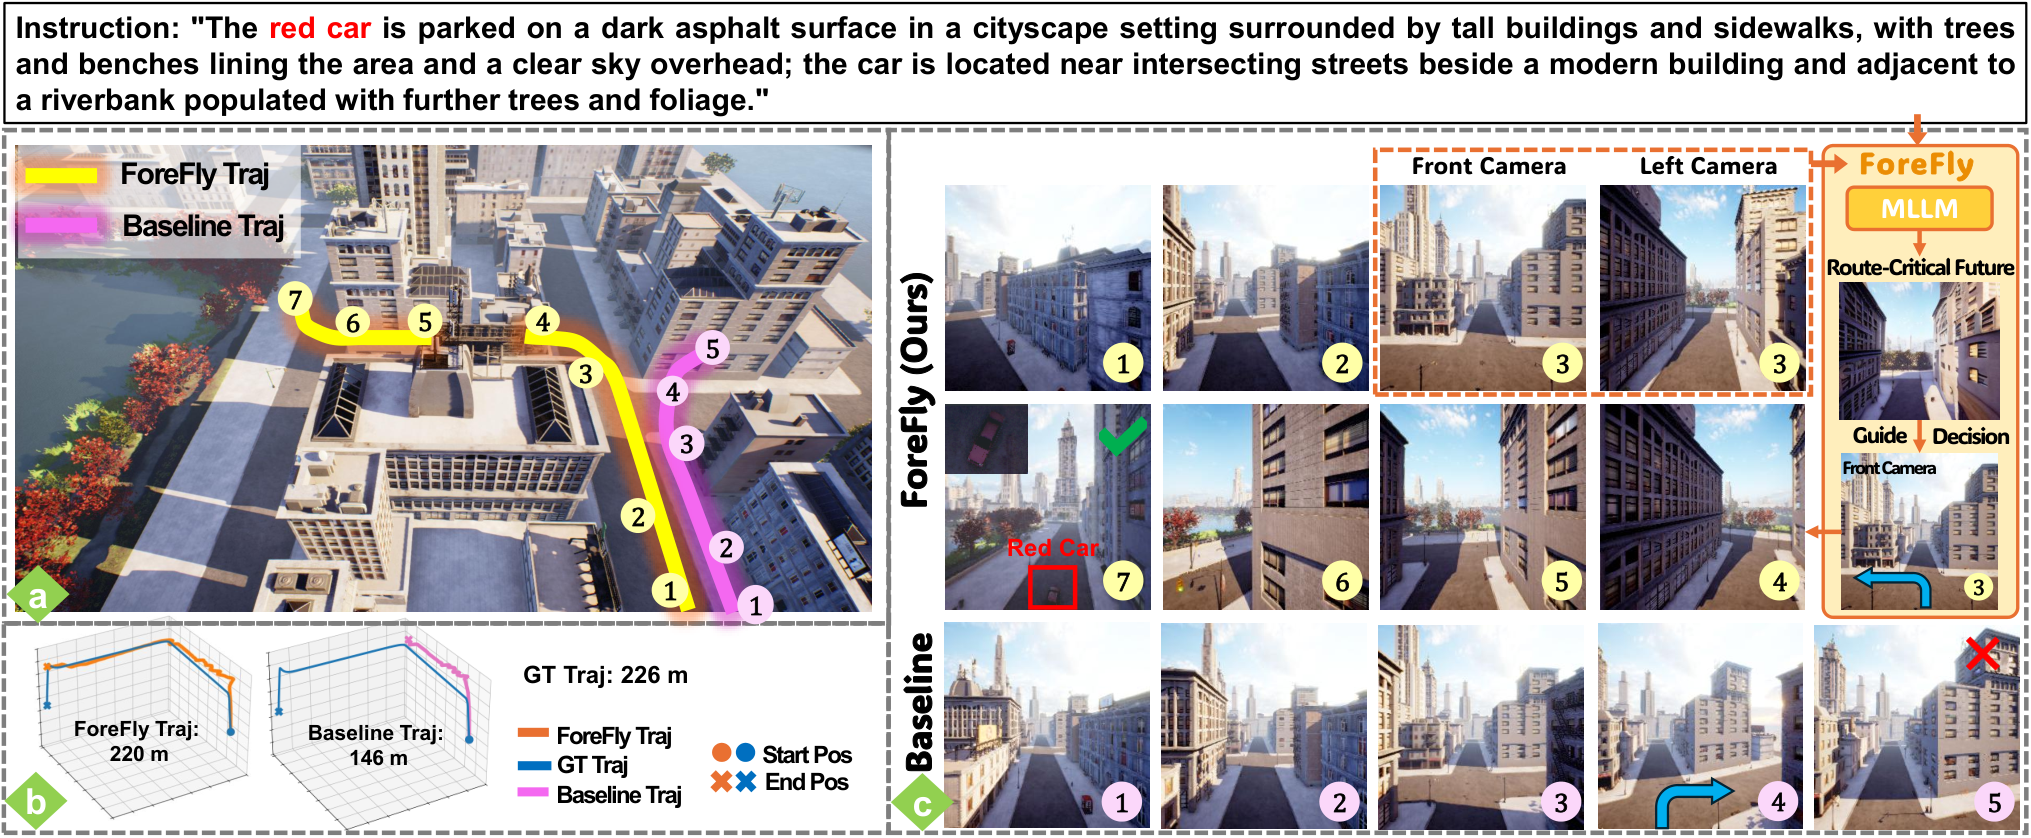
\includegraphics[width=\linewidth,height=26.0mm,keepaspectratio]{figures/p_forefly_case.png}\par{\fontsize{6.6}{8}\selectfont\color{muted}ForeFly · Figure 3（论文原图）}\par\endgroup\vspace{1mm}
{\fontsize{8.0}{10.1}\selectfont
\rowcolors{2}{white}{zebra}
\begin{tabularx}{\linewidth}{@{}Y{1.2}Z{0.69}Y{1.11}@{}}\toprule
\rowcolor{navy}\thd{TravelUAV条件} & \thd{Seen SR（\%）} & \thd{变化}\\\midrule
基线 \ensuremath{\to} 双未来 \ensuremath{\to} ＋query priming & 21.73 \ensuremath{\to} 32.75 \ensuremath{\to} 33.08 & 先加预测，再加记忆初始化\\
直接拼接／去路线bias／完整 & 34.00 ／ 38.35 ／ 41.75 & 融合方式和路线偏置各贡献一截\\
完整Unseen SR & 28.86 & 泛化落差仍在；UAV-ON Seen／Unseen为25.13／22.68\\
\bottomrule\end{tabularx}\par}
\takeaway{同协议中，双未来将SR由21.73升至32.75，完整非对称融合进一步升至41.75，融合方式决定预测的动作价值。}

\note{上面是220米的转弯案例，示范轨迹226米，只作定性展示。表里的数来自TravelUAV：基线21.73，加双未来32.75，再加query priming 33.08；直接拼接双未来34.00，去掉路线bias 38.35，完整41.75。Unseen 28.86，泛化落差单独看。关键事件锚由20度转弯、30米路程等规则定义。}
\end{frame}
\gdef\slidesource{原文依据：\href{https://arxiv.org/html/2605.15964v1}{[16] WorldVLN}}
\begin{frame}[t,label=worldvln]{WorldVLN：世界转移表征直接解码动作}
\relax
\par\begingroup\centering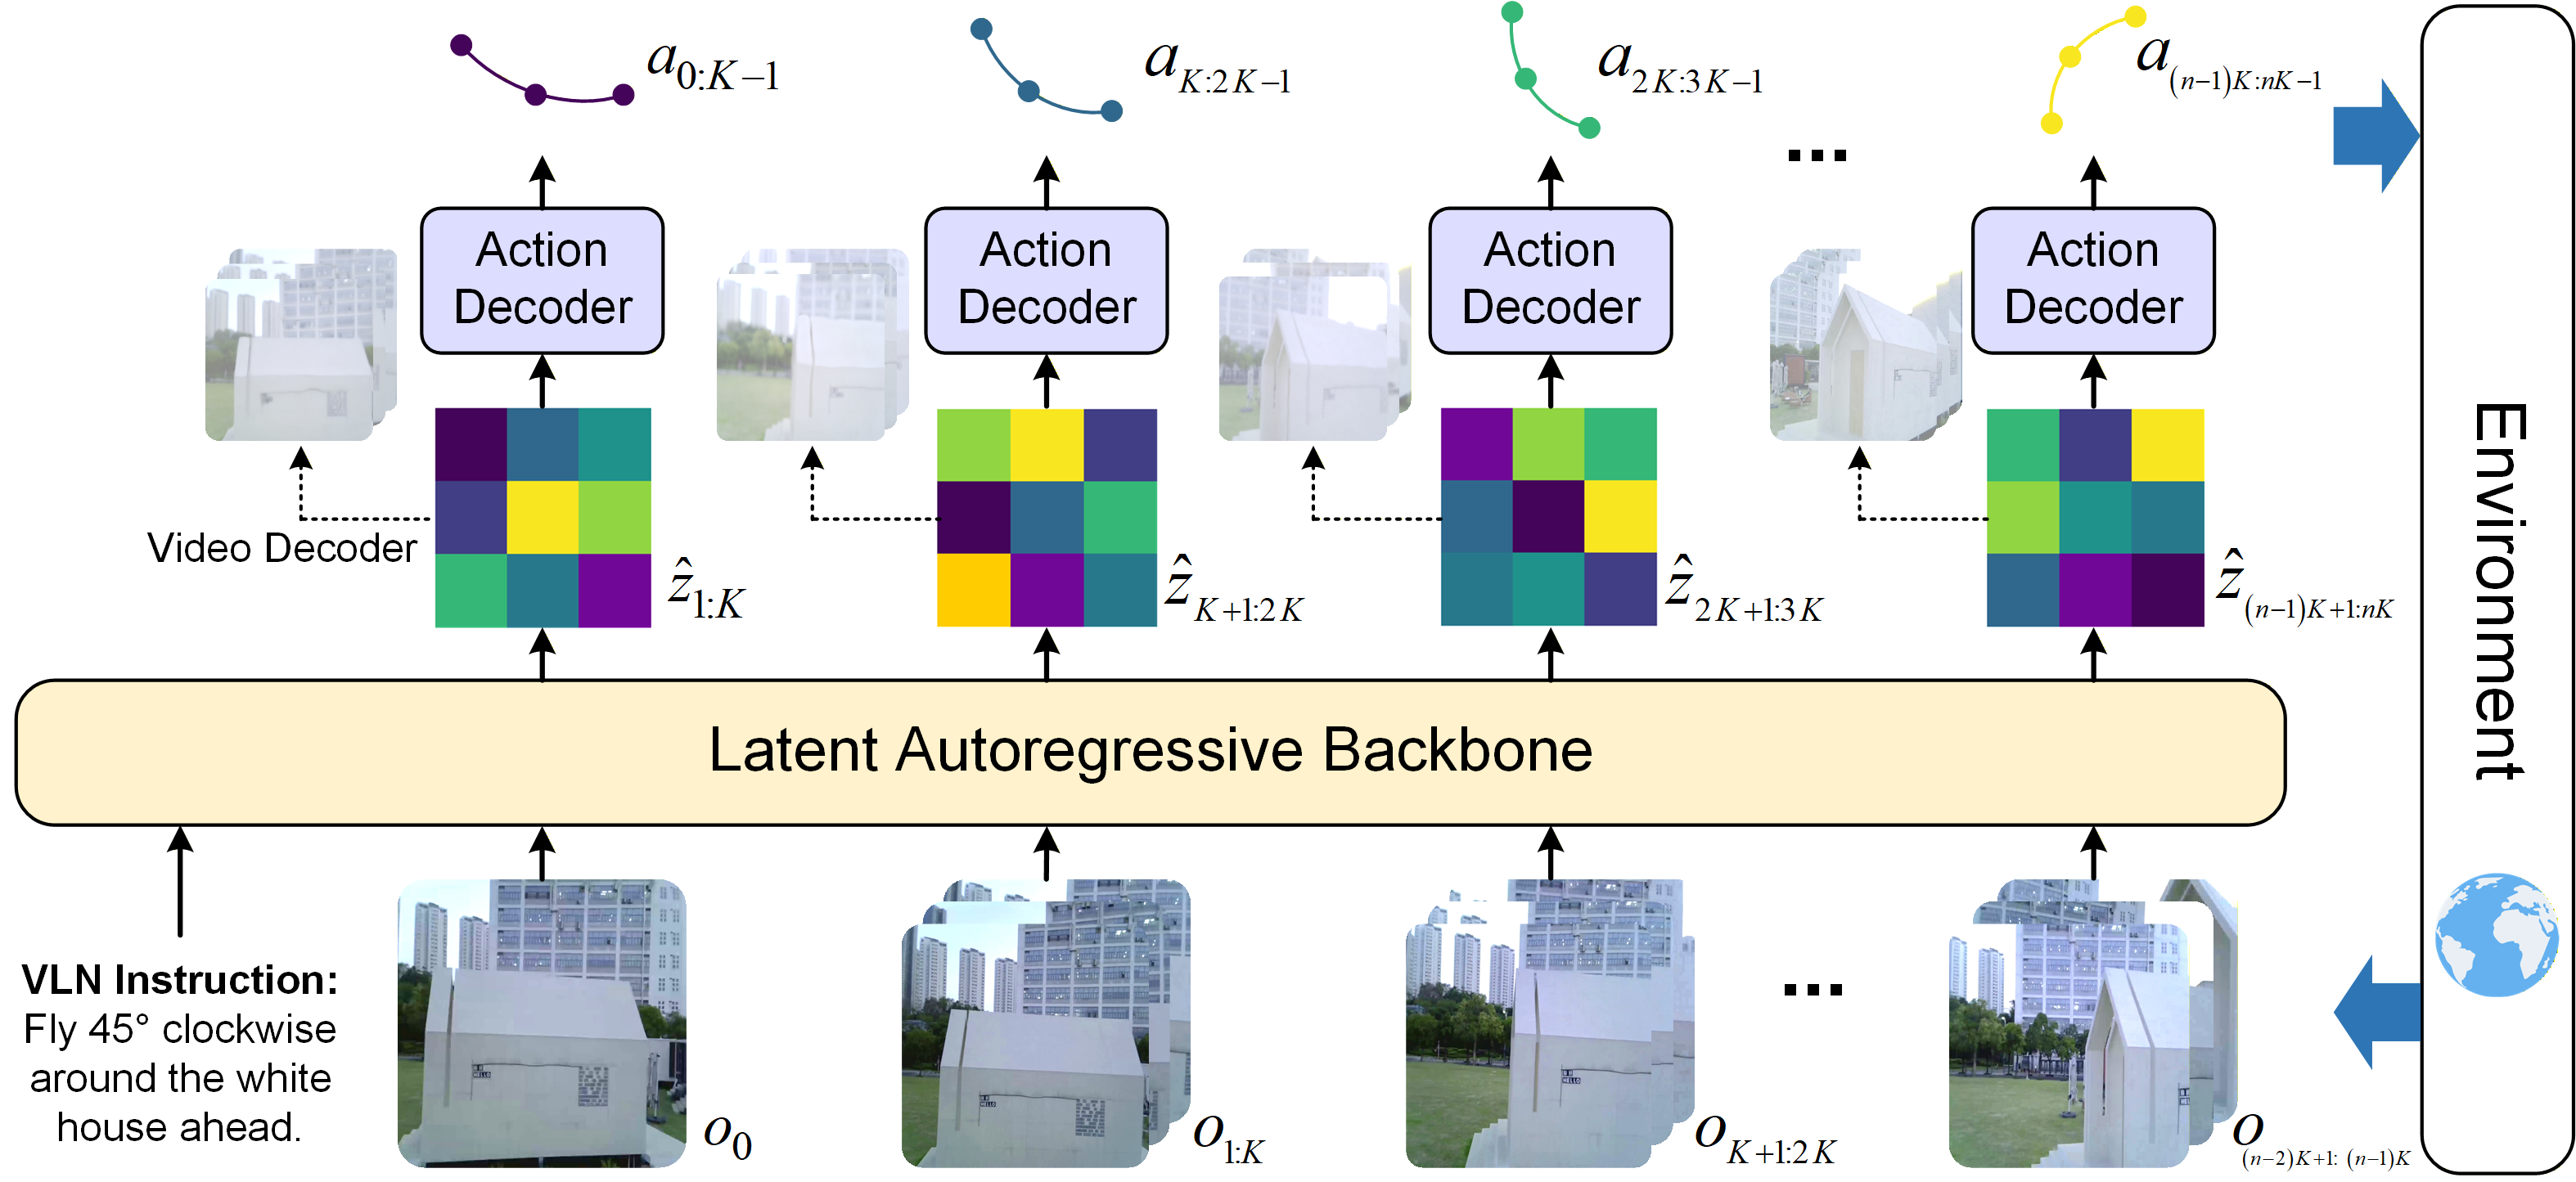
\includegraphics[width=\linewidth,height=25.5mm,keepaspectratio]{figures/p_worldvln.png}\par{\fontsize{6.6}{8}\selectfont\color{muted}WorldVLN · Figure 1（论文原图）}\par\endgroup\vspace{1mm}

\noindent\begin{minipage}[t]{0.3233333333333333\linewidth}\vspace{0pt}\raggedright \par\ph{世界与动作}\quad 指令和观测视频编码后，自回归预测短片段世界token；动作解码器恢复3D位移和偏航，在线不必生成RGB。\par\vspace{1mm}
\end{minipage}\hfill
\begin{minipage}[t]{0.3233333333333333\linewidth}\vspace{0pt}\raggedright \par\ph{训练与重锚}\quad InfinityStar骨干，世界／动作联合监督＋轨迹／任务奖励；26K步、8 GPU；执行后用真实新观察替换预测上下文。\par\vspace{1mm}
\end{minipage}\hfill
\begin{minipage}[t]{0.3233333333333333\linewidth}\vspace{0pt}\raggedright \par\ph{结果与设定}\quad 室内SR 41.76 vs \ensuremath{\pi}0 27.16，nDTW 13.48；Flow固定／开放79.12/\allowbreak{}78.02。任务以原子指令和短时域为主。\par\vspace{1mm}
\end{minipage}\par
\takeaway{架构核心：将视频生成latent解释为世界转移，再直接解码相对航点，并用执行后的真实观察刷新上下文。}

\note{WorldVLN把指令和观测编码后，自回归预测短片段的世界token，再由动作解码器恢复3D位移和偏航；在线不需要生成RGB。训练是世界／动作联合监督，之后用仿真轨迹和任务奖励后训练；每次执行后用真实观察替换预测上下文。室内41.76对\ensuremath{\pi}0 27.16，nDTW 13.48；Flow固定／开放79.12/78.02。}
\end{frame}
\gdef\slidesource{\href{https://arxiv.org/html/2605.15964v1}{[16] WorldVLN} · §4.2；Fig.4}
\begin{frame}[t,label=world_ablation]{WorldVLN：自回归结构与执行后奖励的作用}
\relax

\noindent\begin{minipage}[t]{0.59\linewidth}\vspace{0pt}\raggedright \par\begingroup\centering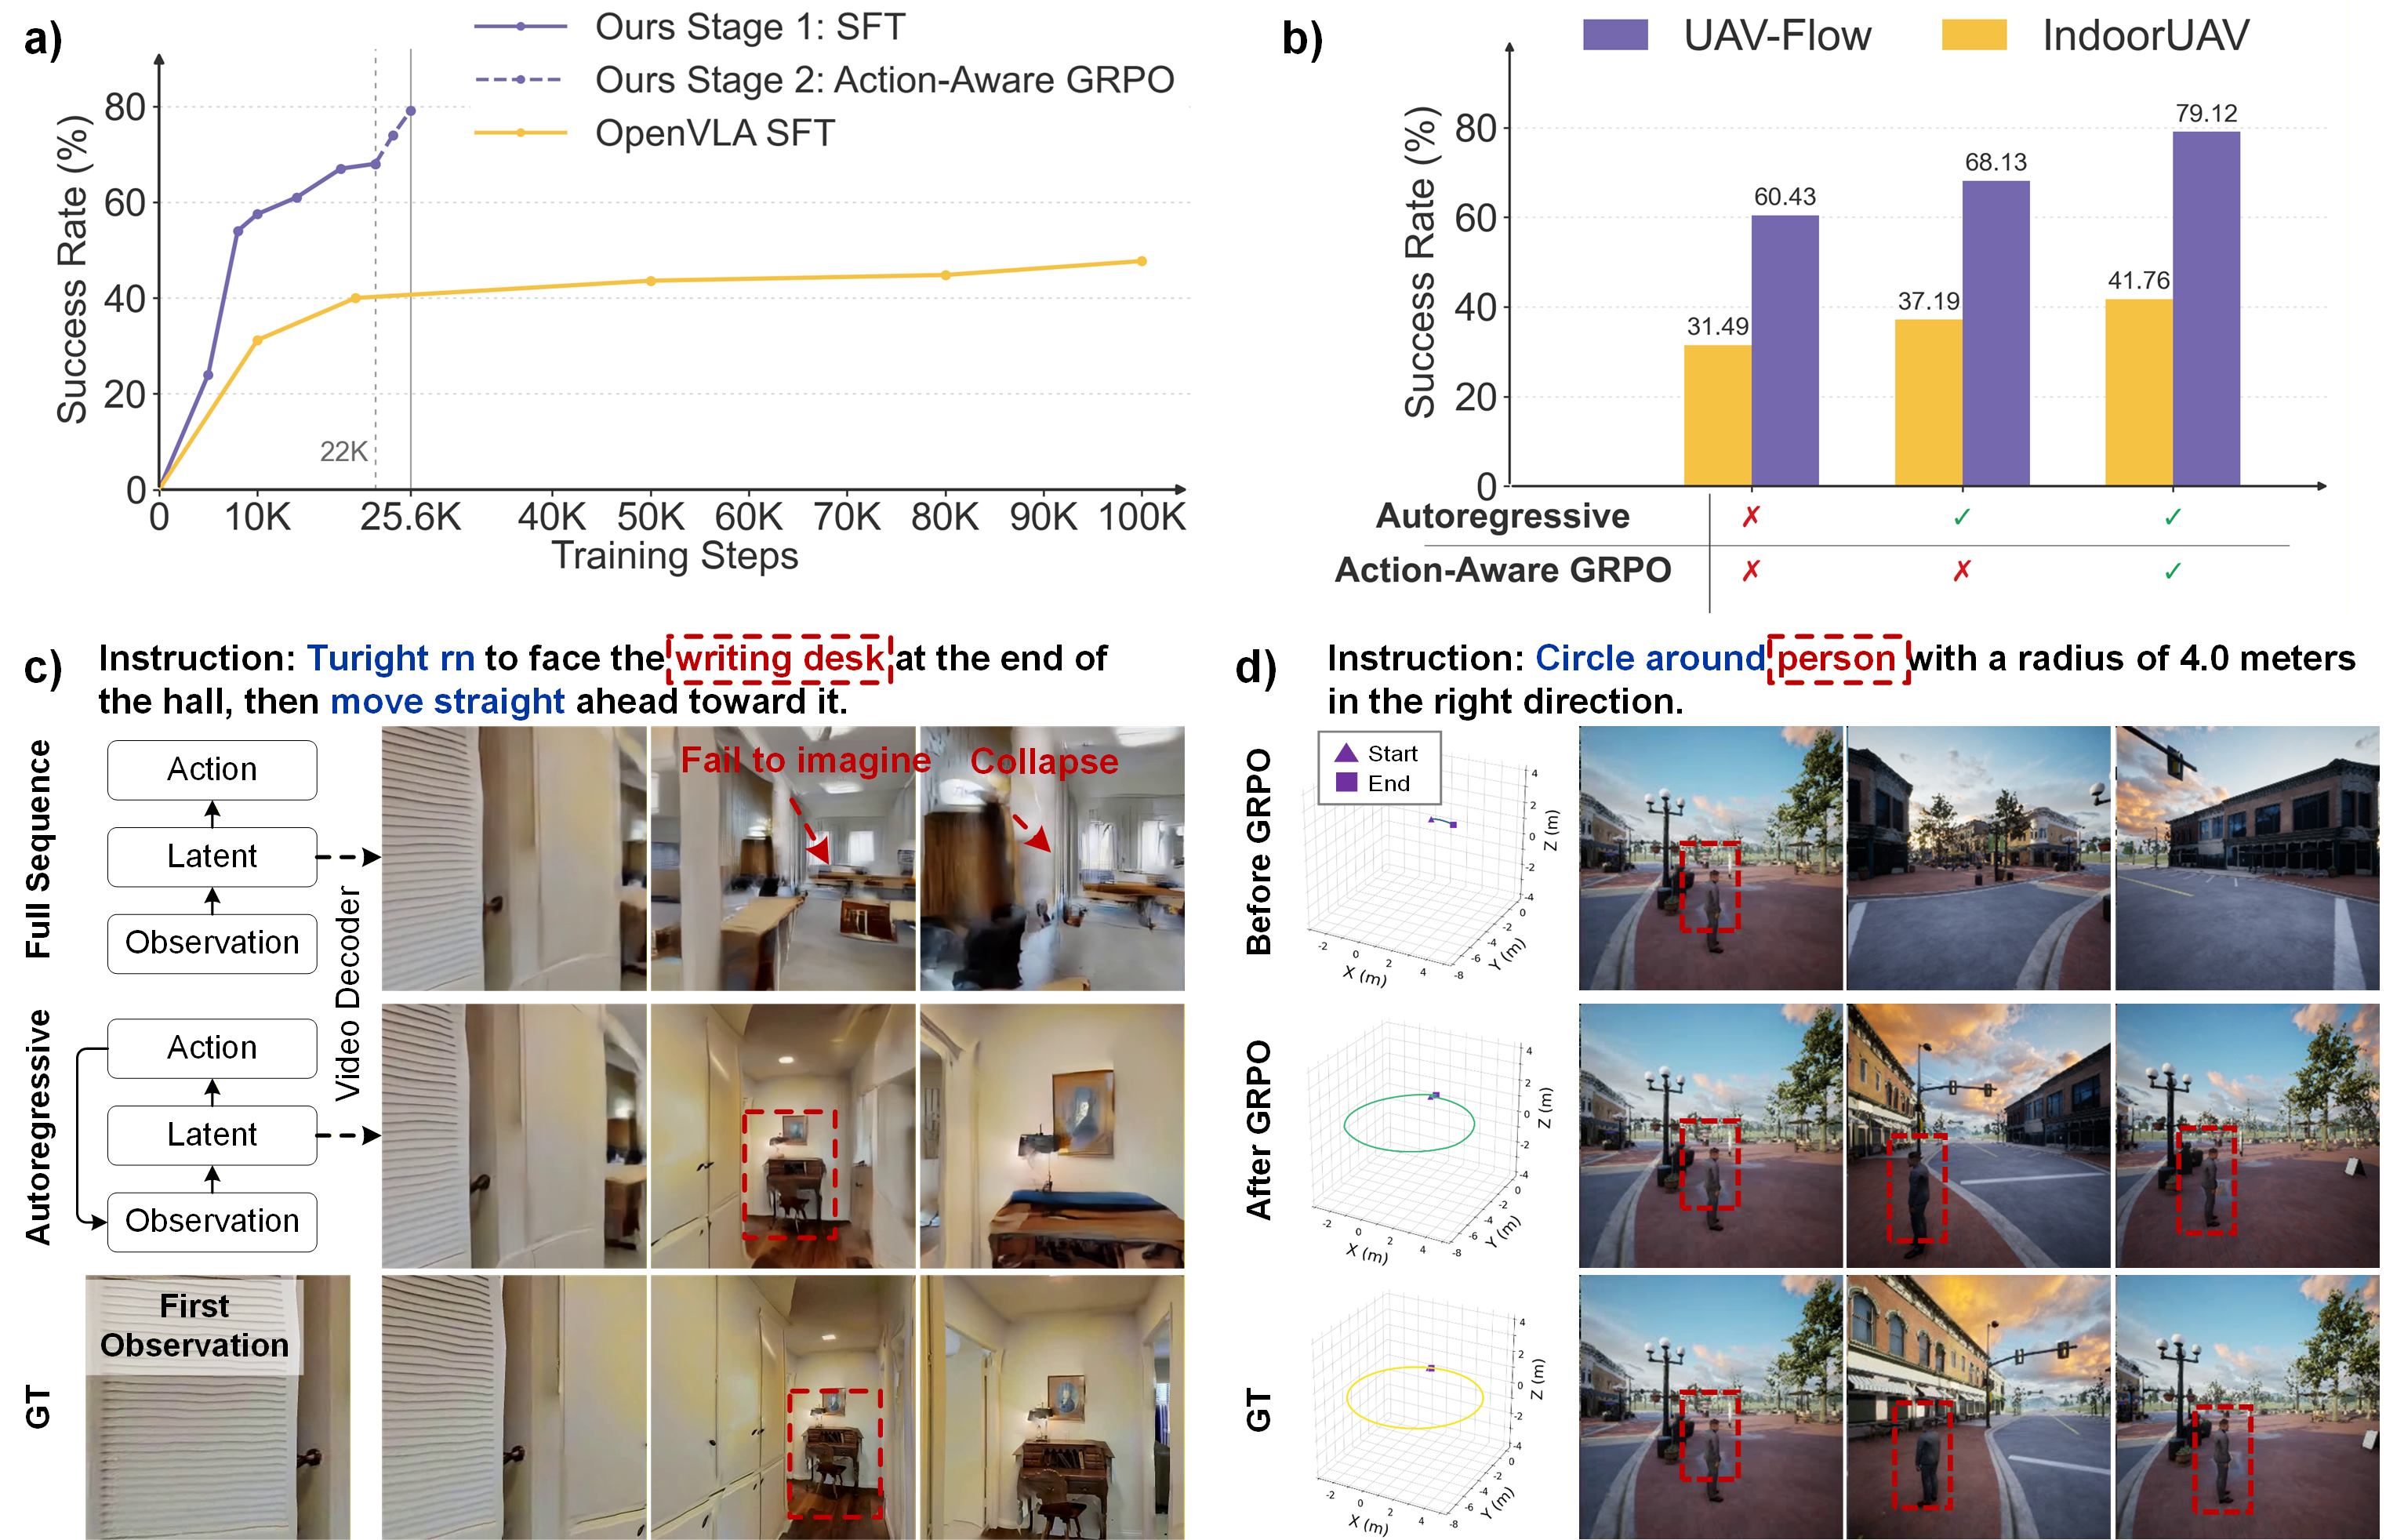
\includegraphics[width=\linewidth,height=20mm,keepaspectratio,trim=0.000bp 281.761bp 0.000bp 0.000bp,clip]{figures/p_worldvln_ablation.png}\par{\fontsize{6.6}{8}\selectfont\color{muted}WorldVLN Fig.4(a,b)：原图局部}\par\endgroup\vspace{.5mm}
\par\begingroup\centering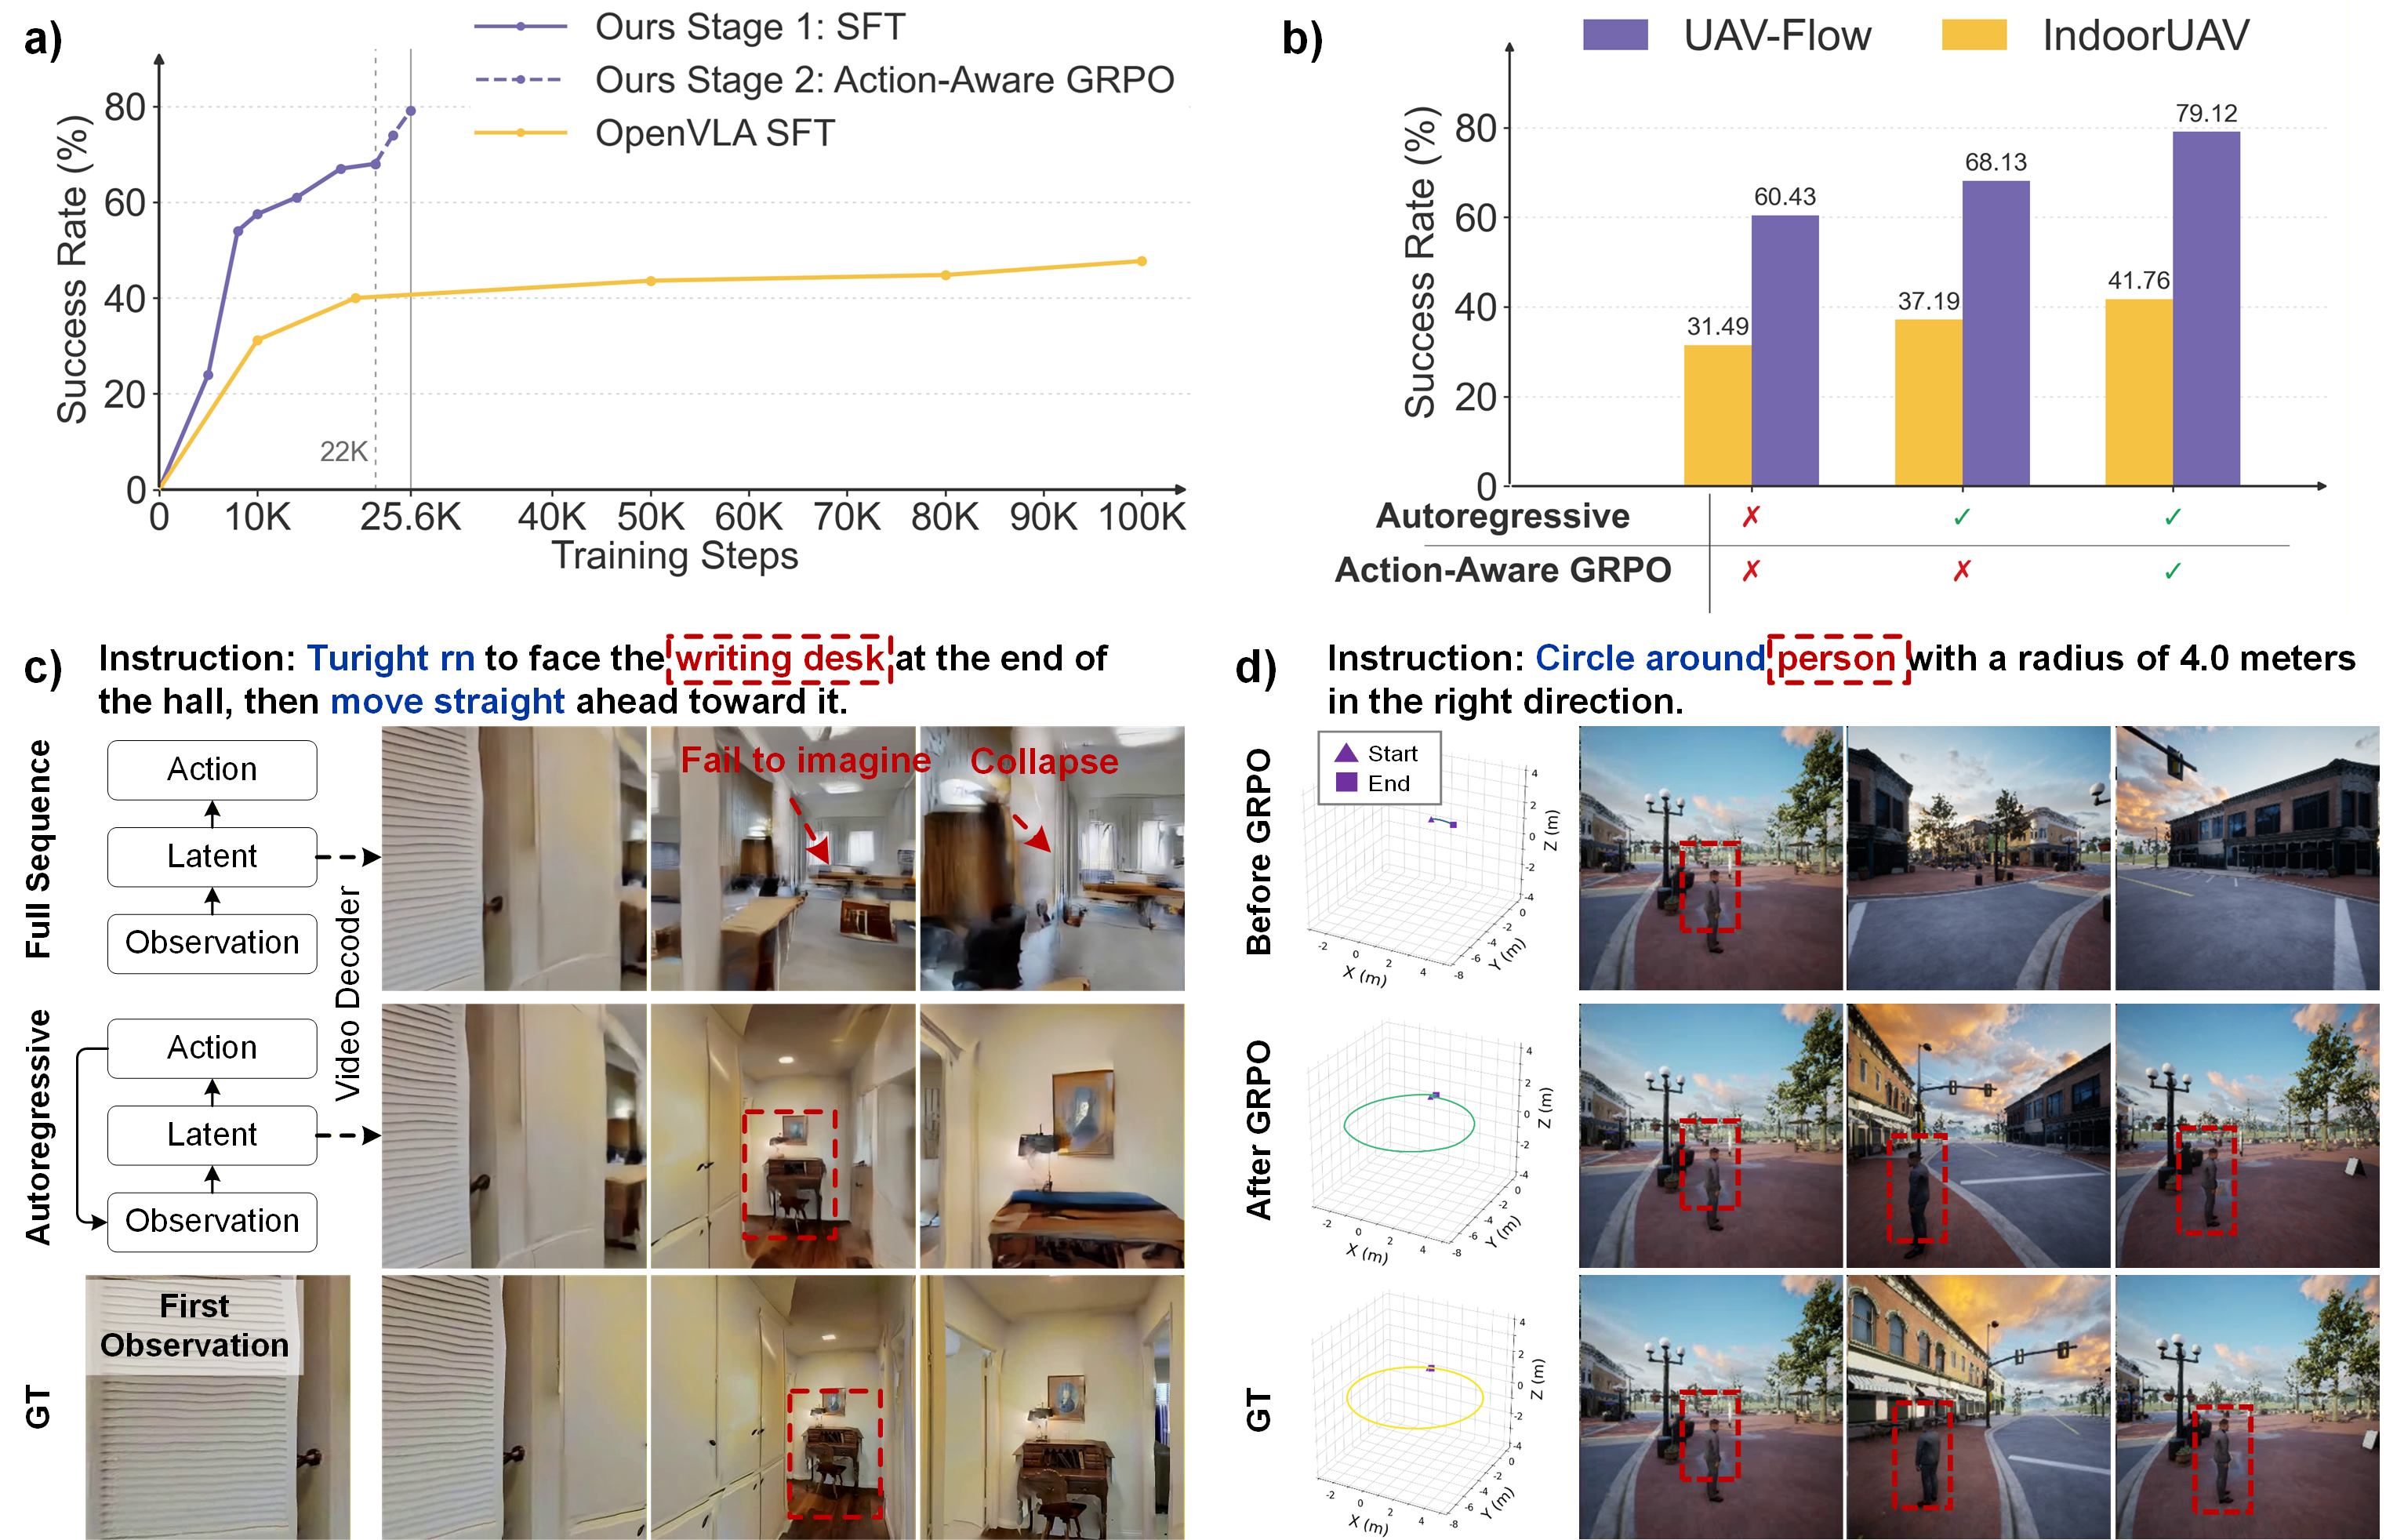
\includegraphics[width=\linewidth,height=21mm,keepaspectratio,trim=0.000bp 0.000bp 0.000bp 192.000bp,clip]{figures/p_worldvln_ablation.png}\par{\fontsize{6.6}{8}\selectfont\color{muted}WorldVLN Fig.4(c,d)：原图局部}\par\endgroup\vspace{.5mm}
\end{minipage}\hfill
\begin{minipage}[t]{0.39\linewidth}\vspace{0pt}\raggedright \par\ph{读图a／b}\quad SFT学习语言条件世界转移与航点解码；GRPO依据实际执行奖励调整策略，自回归结构持续接入真实新观察。\par\vspace{.5mm}
\par\ph{读图c／d}\quad 世界latent保留场景转移，动作头读取位移与yaw；绕行案例展示语言、几何变化与动作方向的对应。\par\vspace{.5mm}
\par\ph{奖励设计}\quad 局部轨迹接近专家、末端目标距离和参考策略约束联合评分；时间衰减给早期决策更大权重。\par\vspace{.5mm}
\end{minipage}\par
\takeaway{世界模型SFT提供可解码的运动先验，在线奖励把这一先验调整到实际执行成功。}

\note{世界骨干以指令视频对学习未来世界latent，动作解码器以真实视频轨迹对学习从世界转移恢复运动。Action-aware GRPO在同一任务上采多条在线rollout，对每个片段综合轨迹接近专家的程度、最终距离目标的程度与参考策略概率，再做组内归一化。时间衰减使前面的决策获得更大权重，因为早期偏航会影响更多后续观察。Figure4分别分析自回归生成、训练收益与可视化解释。}
\end{frame}
\gdef\slidesource{\href{https://arxiv.org/html/2606.01205v2}{[19] ImagineUAV} · §III–IV；Fig.2；Tables I–III}
\begin{frame}[t,label=imagineuav]{ImagineUAV：生成未来视频，再恢复相机运动}
\relax
\par\begingroup\centering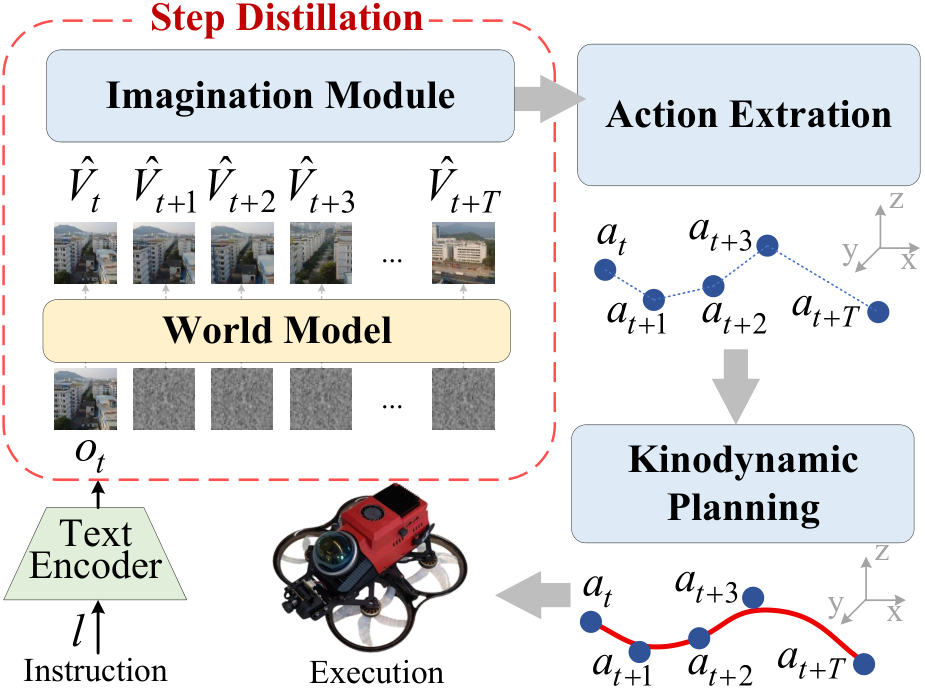
\includegraphics[width=\linewidth,height=27.0mm,keepaspectratio]{figures/p_imagineuav.png}\par{\fontsize{6.6}{8}\selectfont\color{muted}ImagineUAV Fig.2：想象、动作提取与动力学规划}\par\endgroup\vspace{1mm}

\noindent\begin{minipage}[t]{.323\linewidth}\vspace{0pt}\raggedright \ph{语言到未来}\quad Wan2.1 1.3B图像条件视频模型根据当前图与指令生成未来FPV；遮掉相机控制latent，使运动意图主要由语言驱动。\par\end{minipage}\hfill\begin{minipage}[t]{.323\linewidth}\vspace{0pt}\raggedright \ph{未来到动作}\quad Transformer视觉里程计从想象片段回归相对平移与旋转；累积成轨迹后，用B样条优化平滑、避障、可行性与参考偏差。\par\end{minipage}\hfill\begin{minipage}[t]{.323\linewidth}\vspace{0pt}\raggedright \ph{实验与成本}\quad 完整生成SR70.9\%、14.7s；10步蒸馏68.9\%、6.2s。实机带规划13/20完成，去规划9/20。\par\end{minipage}
\takeaway{方法要点：用视觉生成先验承担语义到几何运动的桥梁，再由实测局部地图和轨迹优化完成执行适配。}
\note{想象模块以扩散噪声预测损失训练；动作提取器从短视频和真实相对6DoF运动对学习平移与旋转的L1回归。滑窗处理生成视频后，低置信片段平滑，再将运动参考交给局部规划器。规划代价包含控制点二阶差分、ESDF障碍距离、速度加速度违反和到想象路径的偏差，由L-BFGS优化。10步蒸馏减少视频生成开销；6.2秒包含3.2秒想象及3.0秒动作提取，对应PRO6000。真实部署机载Orin NX运行定位和规划，外部边缘GPU生成未来。实机20次试验对比支持规划器对执行的重要性。}
\end{frame}
\gdef\slidesource{原文依据：\href{https://arxiv.org/html/2609.39763v1}{[20] DiffWAM}}
\begin{frame}[t,label=diffwam]{DiffWAM：早期生成特征读出米制运动}
\relax

\noindent\begin{minipage}[t]{0.57\linewidth}\vspace{0pt}\raggedright \par\begingroup\centering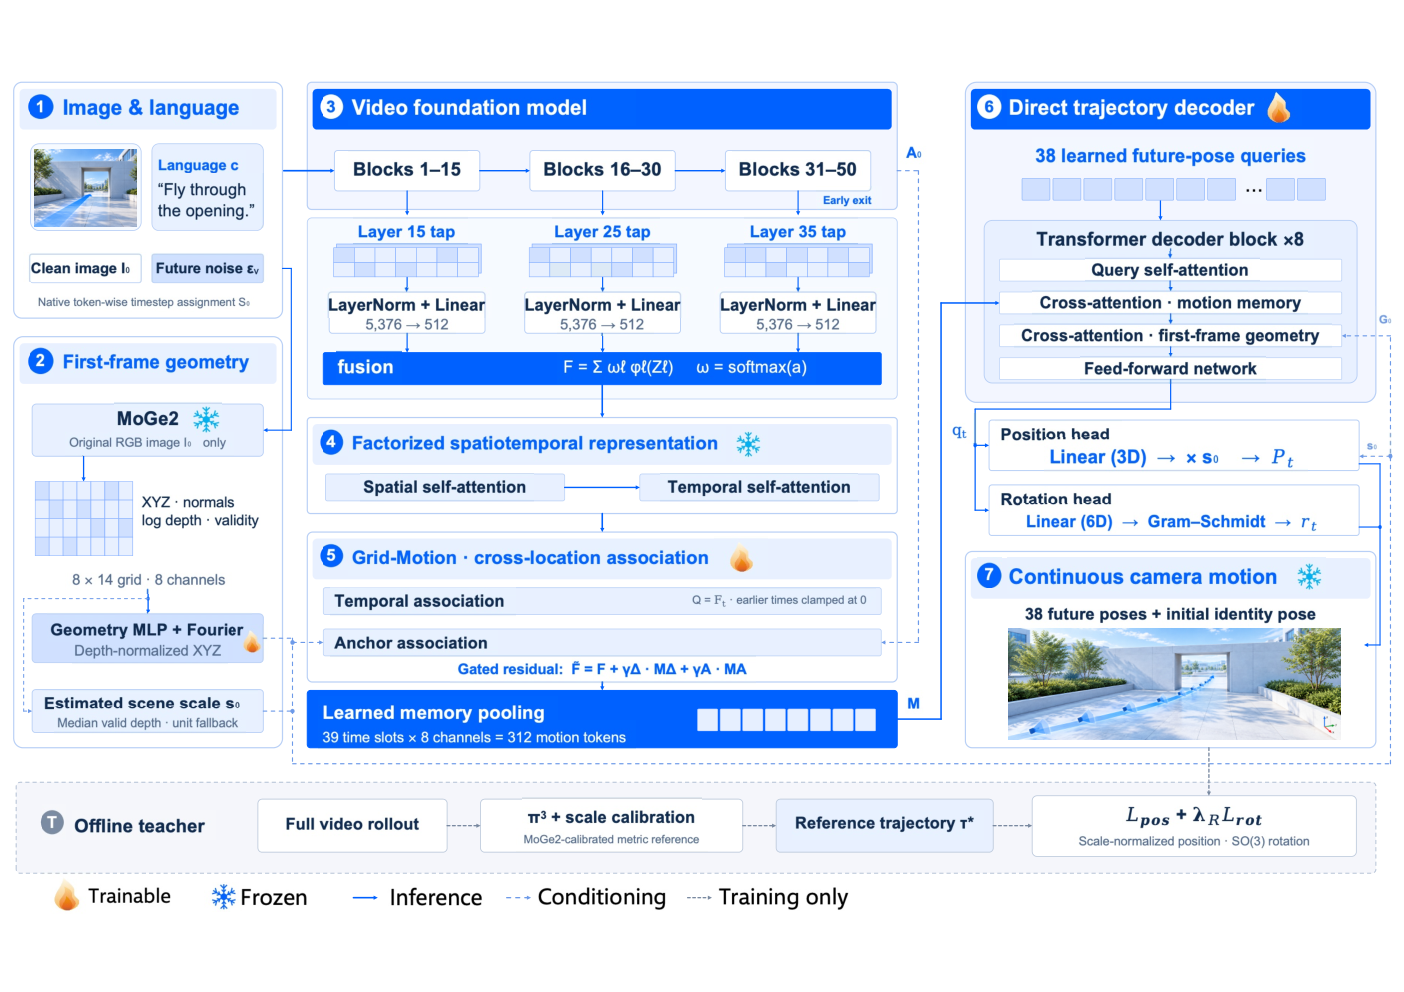
\includegraphics[width=\linewidth,height=42mm,keepaspectratio]{figures/p_diffwam.png}\par{\fontsize{6.6}{8}\selectfont\color{muted}DiffWAM · Figure 3（论文原图）}\par\endgroup\vspace{1mm}
\end{minipage}\hfill
\begin{minipage}[t]{0.41\linewidth}\vspace{0pt}\raggedright {\fontsize{8.9}{11.0}\selectfont\par\ph{冻结与聚合}\quad 取DiT第15/\allowbreak{}25/\allowbreak{}35层早期状态；Grid-Motion关联时空与干净观察锚，聚成312个运动记忆单元。训练用FlyMirage＋NavGen共510K样本。\par\vspace{0.6mm}
\par\ph{几何与解码}\quad 首帧几何写入anchor value；38个查询经8层解码器读运动／几何，尺度恢复平移，6D旋转正交化。\par\vspace{0.7mm}
\par\ph{教师与学生}\quad 完整生成／重建教师做同噪声蒸馏；教师尺度和学生首帧几何是两套条件，分开用。\par\vspace{0.7mm}
\par\ph{输出怎么用}\quad 38个未来位姿加初始共39个；位姿参考还要跟踪和可行性检查，不天然满足动力学。\par\vspace{0.7mm}}
\end{minipage}\par
\takeaway{架构核心：在视频解码前读取预测中的运动，再用首帧几何确定坐标与尺度，直接生成相机轨迹。}

\note{标准DiffWAM保留视频骨干4次早期去噪计算，Flash仅保留第1次；从每次计算的DiT15、25、35层提取特征，最后一次在35层结束。冻结时空前端之后，Grid-Motion先在原始空间网格上关联不同视频时刻与干净观察锚，再池化为312个运动token。首帧MoGe2几何形成坐标、法向、深度及有效性条件；38个查询经8层解码器依次读运动和几何，预测平移与6D旋转并正交化，得到相对初始相机的未来轨迹。训练先做导航运动读出，再用同噪声完整生成与离线重建的教师轨迹蒸馏。部署省去未来RGB解码和多帧重建。}
\end{frame}
\gdef\slidesource{原文依据：\href{https://arxiv.org/html/2606.01205v2}{[19] ImagineUAV}；\href{https://arxiv.org/html/2609.39763v1}{[20] DiffWAM}}
\begin{frame}[t,label=geometry_readout]{运动读出的演进：完整视频恢复与早期特征解码}
\relax
{\fontsize{8.7}{11.1}\selectfont
\rowcolors{2}{white}{zebra}
\begin{tabularx}{\linewidth}{@{}Y{0.69}Y{1.29}Y{1.02}@{}}\toprule
\rowcolor{navy}\thd{比较维度} & \thd{ImagineUAV} & \thd{DiffWAM}\\\midrule
读出方式 & 生成视频 \ensuremath{\to} 学习VO \ensuremath{\to} B样条规划 & 早期DiT \ensuremath{\to} 运动记忆 \ensuremath{\to} 米制SE(3)参考\\
评价配置 & 未蒸馏70.9\%；蒸馏68.9\%／6.2s & 共同端点评价SR 74.40\%\\
真实任务 & 13/\allowbreak{}20 vs 9/\allowbreak{}20，小样本 & 9个实机案例展示不同运动行为\\
几何条件 & 学习VO从视频回归相对位姿 & MoGe2首帧几何提供坐标与尺度\\
执行后端 & 外部生成，机载规划与跟踪 & FastDreamer做异步计划与状态交接\\
架构优势 & 视频动态先验与局部规划明确分工 & 直接动作读出省去视频解码与重建\\
\bottomrule\end{tabularx}\par}
\takeaway{计算路径正在缩短：生成视频→读运动，发展为直接从生成过程中的预测特征读运动。}

\note{ImagineUAV的运动提取器处理完整生成的视频，因此计算包括视频扩散和视觉里程计；DiffWAM让运动读出头读取早期DiT特征，以首帧几何条件恢复尺度。前者的学习分工更清晰，后者减少部署时的生成和重建开销。执行系统都需要处理参考轨迹、局部地图、控制约束与计划时序。表中DiffWAM使用共同终点评价74.40，ImagineUAV蒸馏结果68.9与6.2秒为同一配置；具体任务完成率应采用各论文原任务协议。}
\end{frame}
\section{闭环学习与连续执行}
\gdef\slidesource{\href{https://arxiv.org/html/2608.09467v3}{[21] RefineFly} · Method；Tables 1–4；Appendices}
\begin{frame}[t,label=refinefly]{RefineFly：把未解决失败持续送回在线训练}
\relax
\par\begingroup\centering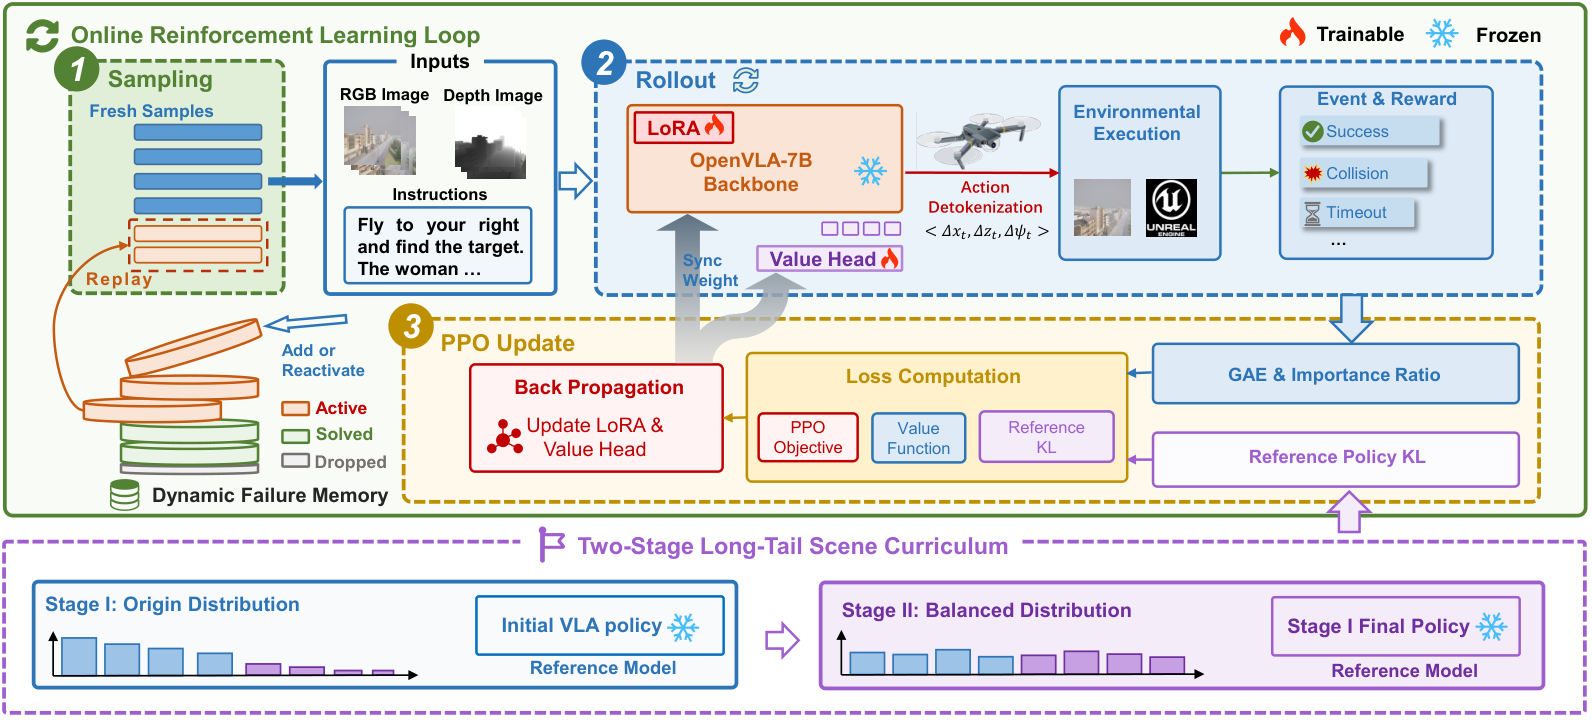
\includegraphics[width=\linewidth,height=26.5mm,keepaspectratio]{figures/p_refinefly.png}\par{\fontsize{6.6}{8}\selectfont\color{muted}RefineFly Fig.2：失败记忆、场景课程与参考策略约束}\par\endgroup\vspace{1mm}

\noindent\begin{minipage}[t]{.323\linewidth}\vspace{0pt}\raggedright \ph{策略与奖励}\quad 保留AerialVLA自回归动作接口，以token级PPO更新；距离进展与碰撞、卡住、远离、早停、超时等事件构成反馈。\par\end{minipage}\hfill\begin{minipage}[t]{.323\linewidth}\vspace{0pt}\raggedright \ph{失败与课程}\quad 记忆存任务初始化和失败类型，每次用当前策略重新执行；成功移出、重试超限丢弃。先按经验场景分布，再按场景均衡采样。\par\end{minipage}\hfill\begin{minipage}[t]{.323\linewidth}\vspace{0pt}\raggedright \ph{稳定性与结果}\quad 每阶段固定参考策略做KL约束。Seen / 未见地图 / 未见对象SR为56.33 / 42.97 / 59.72；基线47.96 / 37.58 / 56.60。\par\end{minipage}
\takeaway{方法要点：重试失败任务提供针对性，场景均衡提供覆盖，阶段参考策略限制反复适配造成的策略漂移。}
\note{失败记忆保存任务初始化、场景、失败类型、状态和重试次数，而不是将旧轨迹直接当成在线PPO数据。选中任务后必须用当前策略重新rollout，因此概率与奖励都来自当前训练过程。课程阶段I按训练任务数量分配场景，阶段II按场景均匀分配；两阶段均预留部分任务给未解决失败。阶段I参考是初始VLA，阶段II参考是阶段I末策略。PPO对有效动作token独立裁剪，并按命令有效token数归一化，value head和GAE提供动作级优势。表1–3为三个评价种子的均值；增量消融表4采用单个评价种子。}
\end{frame}
\gdef\slidesource{\href{https://arxiv.org/html/2608.09467v3}{[21] RefineFly} · Table 4；固定评价seed 1；SR（\%）}
\begin{frame}[t,label=refinefly_ablation]{RefineFly消融：失败重试需要场景课程配合}
\relax
{\fontsize{8.5}{10.8}\selectfont\rowcolors{2}{white}{zebra}
\begin{tabularx}{\linewidth}{@{}Y{1.5}Y{0.8}Y{0.85}Y{0.85}@{}}\toprule\rowcolor{navy}\thd{配置} & \thd{Seen SR} & \thd{未见地图SR} & \thd{未见对象SR}\\\midrule
AerialVLA初始化 & 47.96 & 37.58 & 56.60\\
token PPO & 48.17 & 42.90 & 56.44\\
＋失败记忆 & 56.21 & 31.21 & 59.78\\
＋参考KL & 55.01 & 37.47 & 62.32\\
＋两阶段场景课程 & 56.28 & 44.89 & 60.41\\
\bottomrule\end{tabularx}\par}
\bline{为什么仅失败重试会退化}{反复训练当前失败集中出现的地图，会使任务分布进一步偏斜；Seen提升并不保证新场景泛化。}
\bline{课程怎样补足}{在第二阶段重新分配场景训练机会，让稀少场景中的失败也得到处理；参考KL限制策略偏离已有导航能力。}\takeaway{关键发现：闭环学习不仅取决于奖励，还取决于哪些场景、哪些失败在何时被反复看到。}
\note{增量消融中加入失败记忆后未见地图SR42.90降到31.21，加入参考KL回到37.47，再加入场景课程达到44.89；Seen则保持较高水平。这组对照清楚表明失败学习存在分布效应。Table4的44.89是单评价种子，不替换主结果Table2的42.97均值。若扩展到群体训练，应按团队失败类型、场景和角色分布共同调度重试。}
\end{frame}
\gdef\slidesource{\href{https://arxiv.org/html/2606.02313v1}{[22] EG-GRPO} · §3.2–3.5；Tables 1–3}
\begin{frame}[t,label=eggrpo]{EG-GRPO：用专家轨迹建立组内高奖励参照}
\relax
\par\begingroup\centering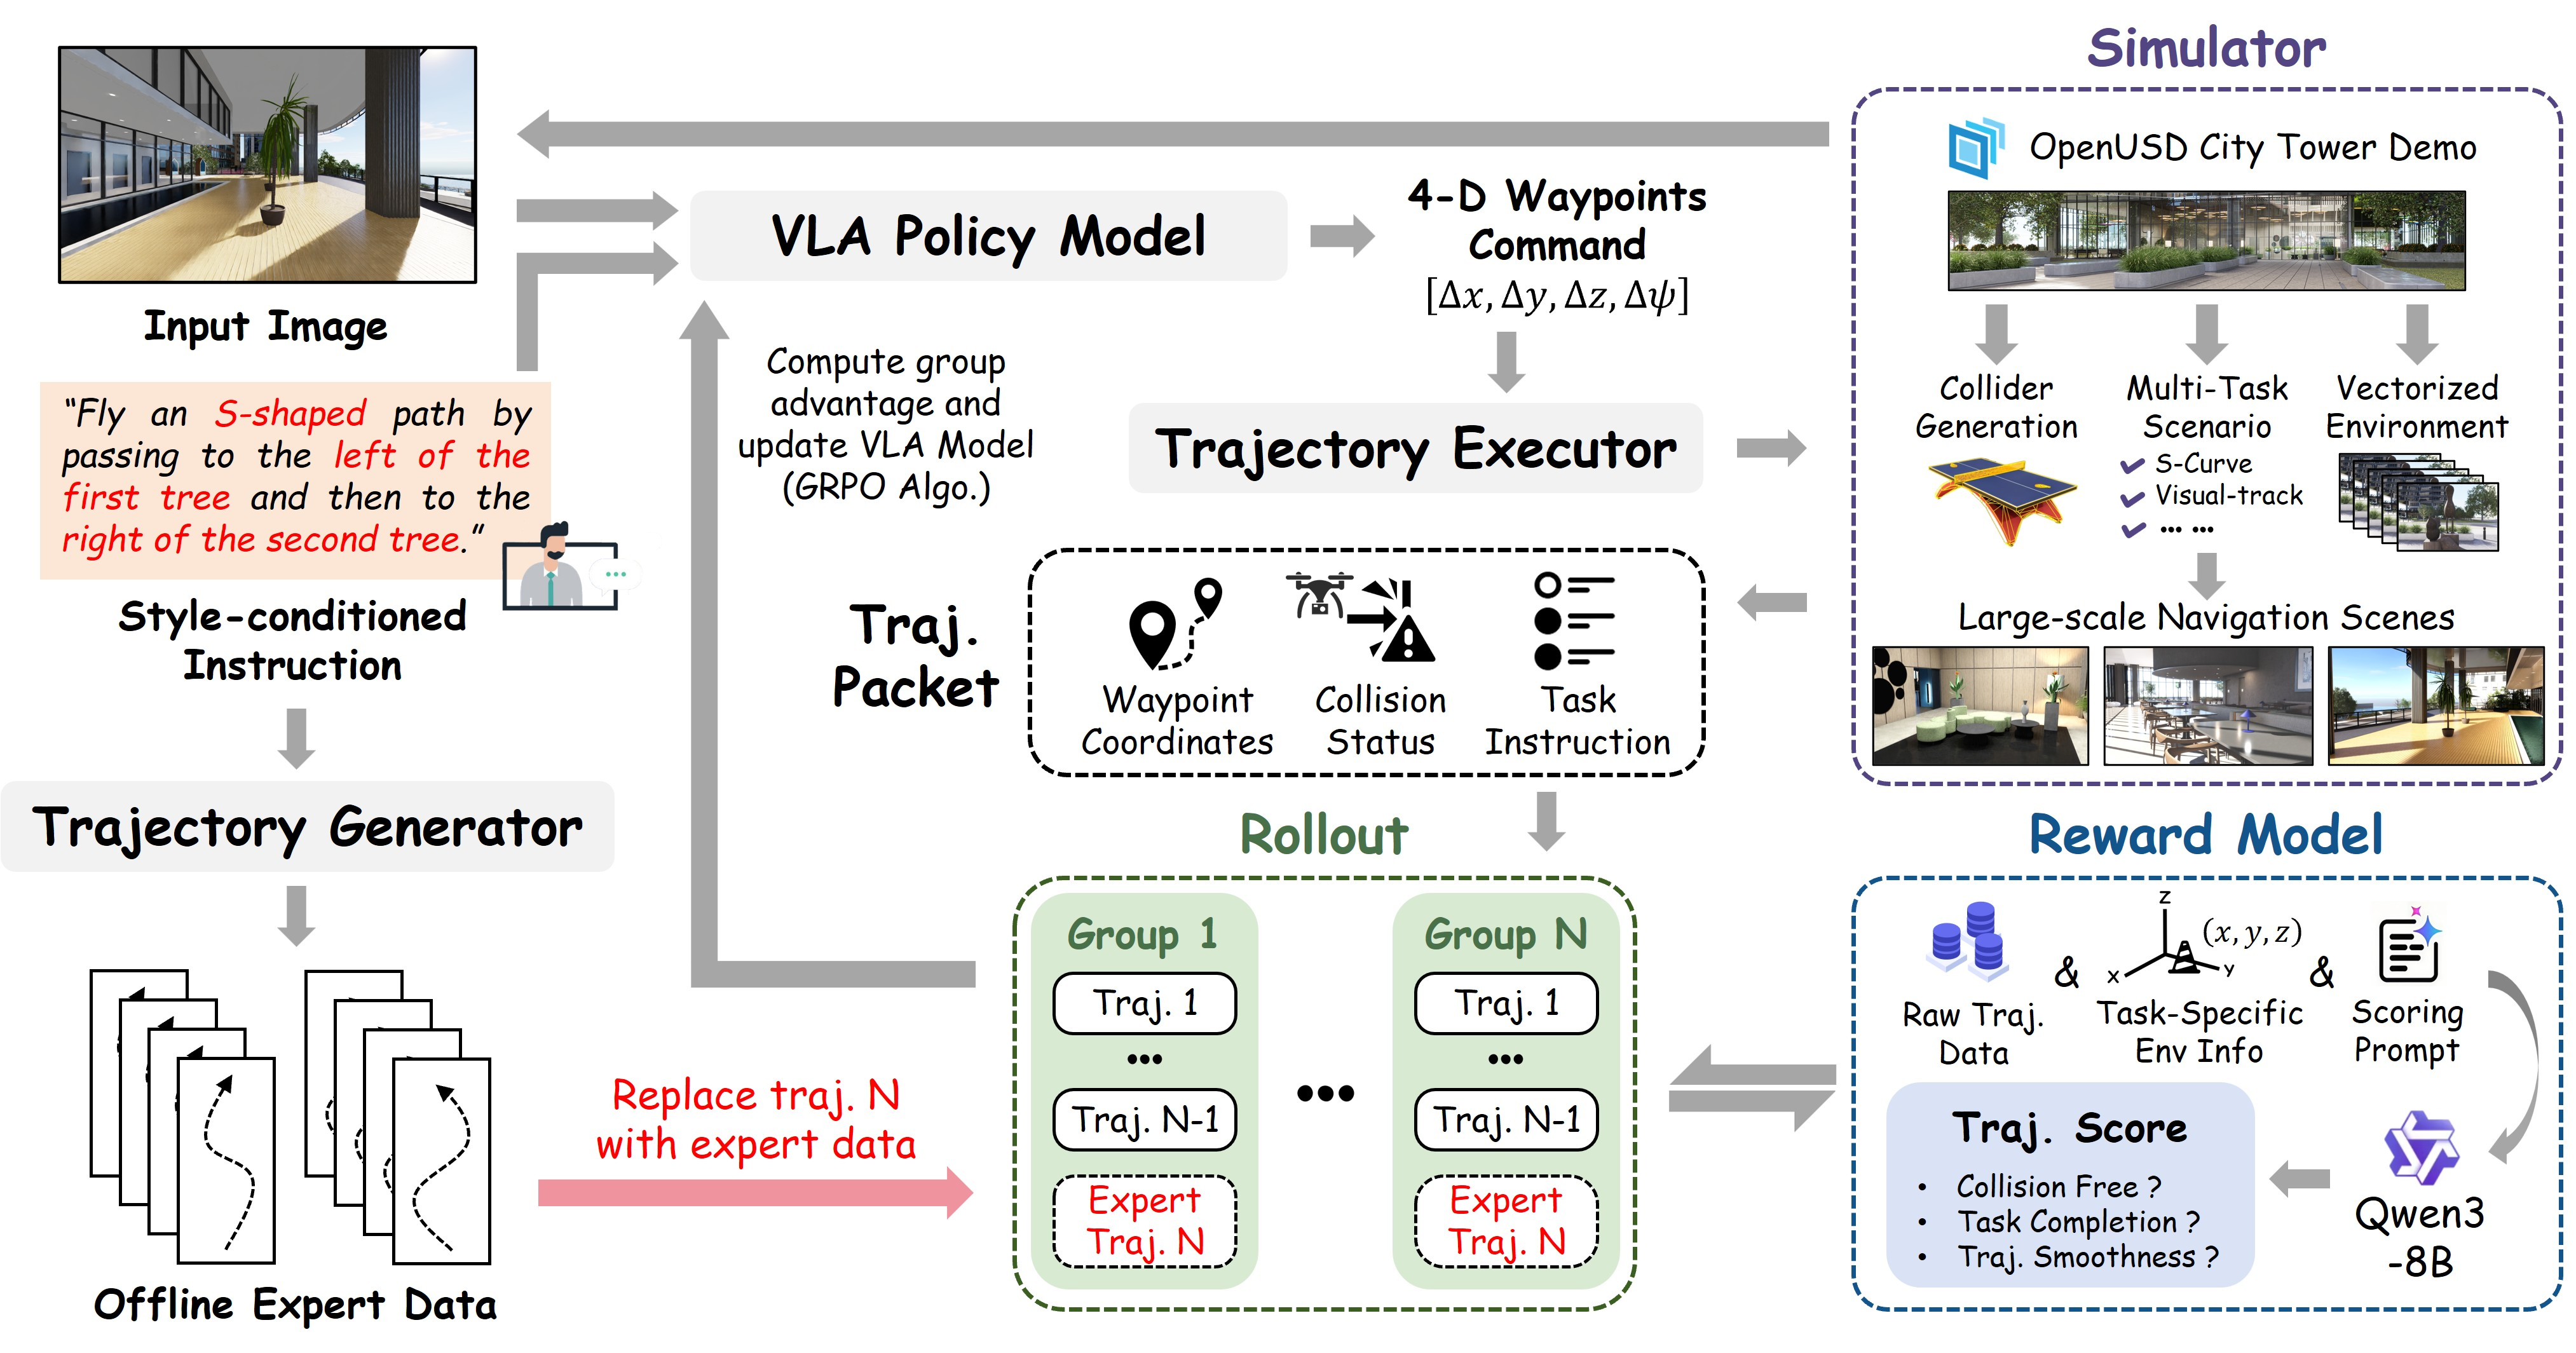
\includegraphics[width=\linewidth,height=26.5mm,keepaspectratio]{figures/p_eggrpo.jpg}\par{\fontsize{6.6}{8}\selectfont\color{muted}EG-GRPO Fig.2：在线rollout、专家注入与意图奖励}\par\endgroup\vspace{1mm}

\noindent\begin{minipage}[t]{.323\linewidth}\vspace{0pt}\raggedright \ph{初始化与目标}\quad OpenVLA-OFT在UAV-Flow上SFT，输出4D运动；指令条件轨迹奖励同时评价任务结果与速度、绕行方式等细粒度意图。\par\end{minipage}\hfill\begin{minipage}[t]{.323\linewidth}\vspace{0pt}\raggedright \ph{专家如何起作用}\quad 每组G−1条在线轨迹加入1条规则专家轨迹，统一算组内均值与方差；专家同时成为相对优势锚点和策略更新样本。\par\end{minipage}\hfill\begin{minipage}[t]{.323\linewidth}\vspace{0pt}\raggedright \ph{实验发现}\quad 难任务SR：SFT18.7→GRPO26.4→EG-GRPO43.1；总体26.1→55.6。异构仿真／推理并行使rollout耗时下降43.5\%。\par\end{minipage}
\takeaway{方法要点：当在线样本都很差时，专家参照提供可区分的相对学习信号，推动复杂意图动作的学习。}
\note{每组混入一条专家轨迹，比例1/G，并将其和在线轨迹一起计算相对优势与clip目标；因此不仅改变采样，也改变组内奖励统计和梯度来源。对专家样本的策略概率同样按当前与旧策略计算，构成混合数据训练。论文采用指令条件轨迹评价器，并将渲染仿真GPU与模型推理GPU分开流水并行。难任务包含S形绕行、上下穿越等初始示范较少的技能；Table2的18.7、26.4、43.1分别对应SFT、普通GRPO、专家注入GRPO，不能把26.4误标成SFT。}
\end{frame}
\gdef\slidesource{\href{https://arxiv.org/html/2610.21450v1}{[23] X-Fly} · §3–4；Fig.3；Tables 1–2}
\begin{frame}[t,label=xfly_arch]{X-Fly：快慢视觉表征、动作块与独立STOP头}
\relax
\par\begingroup\centering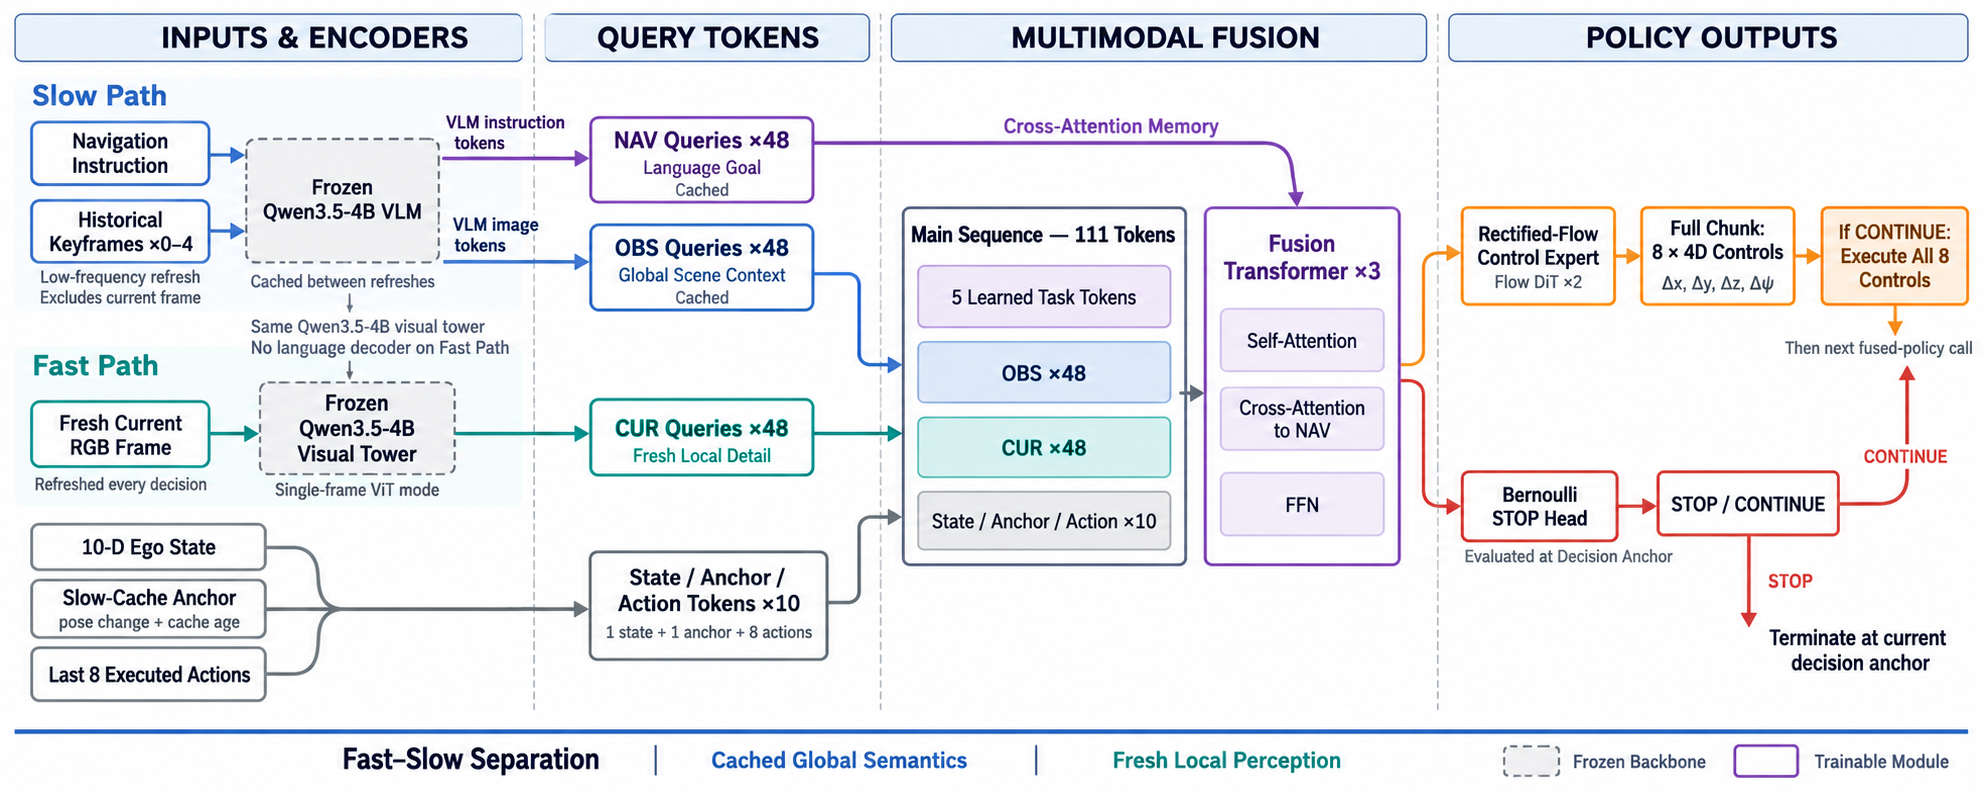
\includegraphics[width=\linewidth,height=26.5mm,keepaspectratio]{figures/p_xfly.png}\par{\fontsize{6.6}{8}\selectfont\color{muted}X-Fly Fig.3：冻结VLM的快慢路径与八步控制器}\par\endgroup\vspace{1mm}

\noindent\begin{minipage}[t]{.323\linewidth}\vspace{0pt}\raggedright \ph{表征与控制}\quad 慢路径缓存指令与因果关键帧，快路径更新当前视觉；融合状态、缓存锚和最近执行动作，经rectified flow生成8个4D控制。\par\end{minipage}\hfill\begin{minipage}[t]{.323\linewidth}\vspace{0pt}\raggedright \ph{训练问题}\quad 八步执行后才再次决策，实际状态偏离专家分布；恢复DAgger在当前策略到达的锚点构造平滑回接块，并补首次到达的STOP标签。\par\end{minipage}\hfill\begin{minipage}[t]{.323\linewidth}\vspace{0pt}\raggedright \ph{闭环收益}\quad Seen：BC全块16.45→恢复63.46→Flow-GRPO74.18；Unseen18.43→40.63→51.73。模型时间摊至每航点42ms。\par\end{minipage}
\takeaway{方法要点：长动作块同时放大控制偏移与终止监督缺口，必须在策略自己的到达状态上学习恢复和停止。}
\note{骨干Qwen3.5-4B与视觉塔均冻结，训练query、融合、flow控制器与STOP头。慢路径每16个已执行航点刷新，快路径在每个决策锚刷新当前图。BC使用849,106专家窗口，部署每次执行完整8个控制；恢复DAgger用单调专家游标保持路线次序，从当前偏移状态构造零端点斜率的三次回接。收集时禁用STOP，首次进入目标范围的锚点标正，后续截断。Flow-GRPO联合调整控制与停止概率，并使用结果验证的停止样本。74.18等结果是条件控制rollout下对首次STOP分布积分得到的期望指标。}
\end{frame}
\gdef\slidesource{原文依据：\href{https://arxiv.org/html/2610.21450v1}{[23] X-Fly}}
\begin{frame}[t,label=xfly]{X-Fly：恢复标签与首次到达停止标签}
\relax
\bline{恢复动作块}{设当前状态偏离专家路线$d_t$，在八步内平滑消去偏移；单调游标$c_t$保持示范顺序，避免自交路线错误回跳。}
\[p^{\rm rec}_{t,j}=p^*_{c_t+j}+d_t(1-3q_j^2+2q_j^3),\qquad q_j=j/H,\quad H=8\]
\bline{到达与STOP}{收集时禁用STOP，记录策略自己的首次目标区内决策锚，赋予STOP＋悬停标签；此前状态继续执行恢复块。}
\bline{三阶段作用}{BC建立视觉动作先验；Recovery DAgger在策略分布中补恢复和停止监督；Flow-GRPO用任务结果调整动作与STOP概率。}
\bline{评价方式}{固定控制rollout后，对首次STOP概率$p_t\prod_{j<t}(1-p_j)$积分，得到SR等条件期望；同配置比较各训练阶段。}
\takeaway{长动作块的收益依赖匹配的训练状态：既要会从偏航中恢复，也要在自己真正到达时学会停止。}
\note{恢复目标在块起点等于当前状态，在终点重新接上未来专家路线，三次偏移衰减在两端具有零斜率。yaw用同类恢复并按最短角度包裹。恢复训练包含三轮收集与训练，每轮与BC数据按1:1混合。首次目标区内锚点标STOP后截断，避免到达后的专家游标给出反向标签。Flow-GRPO进一步加入结果验证的停止辅助监督。}
\end{frame}
\gdef\slidesource{原文依据：\href{https://arxiv.org/html/2608.09467v3}{[21] RefineFly}；\href{https://arxiv.org/html/2606.02313v1}{[22] EG-GRPO}；\href{https://arxiv.org/html/2610.21450v1}{[23] X-Fly}；\href{https://arxiv.org/html/2610.25407v1}{[24] AeroDASH}}
\begin{frame}[t,label=posttraining]{四类后训练分别修复什么问题}
\relax
{\fontsize{9.0}{11.0}\selectfont{\fontsize{8.5}{10.6}\selectfont
\rowcolors{2}{white}{zebra}
\begin{tabularx}{\linewidth}{@{}Y{0.69}Y{1.29}Y{1.02}@{}}\toprule
\rowcolor{navy}\thd{方法} & \thd{学习信号} & \thd{结果与适用条件}\\\midrule
RefineFly & token PPO、失败记忆、课程 & 分布：失败重试＋场景均衡＋参考KL\\
EG-GRPO & G−1在线＋1专家，意图对齐奖励 & Difficult 26.4\ensuremath{\to}43.1；难任务SFT18.7，普通GRPO26.4\\
X-Fly & 恢复状态、停止辅助、控制后训练 & 恢复学习修复偏移与到达锚点监督\\
AeroDASH & group-relative轨迹奖励 & 样条动作经执行后，以nDTW优化路径对齐\\
\bottomrule\end{tabularx}\par}
\par\ph{效率机制}\quad EG将渲染仿真与VLA推理流水并行，使rollout每步耗时由904.67s降至511.01s。\par\vspace{0.4mm}
\par\ph{研究设计}\quad 第一阶段冻结单体策略和回答器，只动观察分配、证据处理和停止规则；这样增益才能落到团队层。\par\vspace{0.4mm}
\takeaway{共同趋势：把专家示范没有覆盖的闭环状态与实际执行后果，重新纳入策略学习。}
}
\note{RefineFly改变任务重试和场景训练分布；EG-GRPO为难任务补充高奖励参照；X-Fly在长块执行诱导的状态上构造恢复和停止标签；AeroDASH通过真实异步执行后的nDTW训练样条策略。这四类方法分别补训练分布、优势参照、状态支持和执行时延。群体研究可以复用这些机制，但应先固定单体后端以隔离团队观察分配带来的作用。}
\end{frame}
\gdef\slidesource{原文依据：\href{https://arxiv.org/html/2610.25407v1}{[24] AeroDASH}}
\begin{frame}[t,label=aero]{AeroDASH：异步推理与连续参考接轨}
\relax
\par\begingroup\centering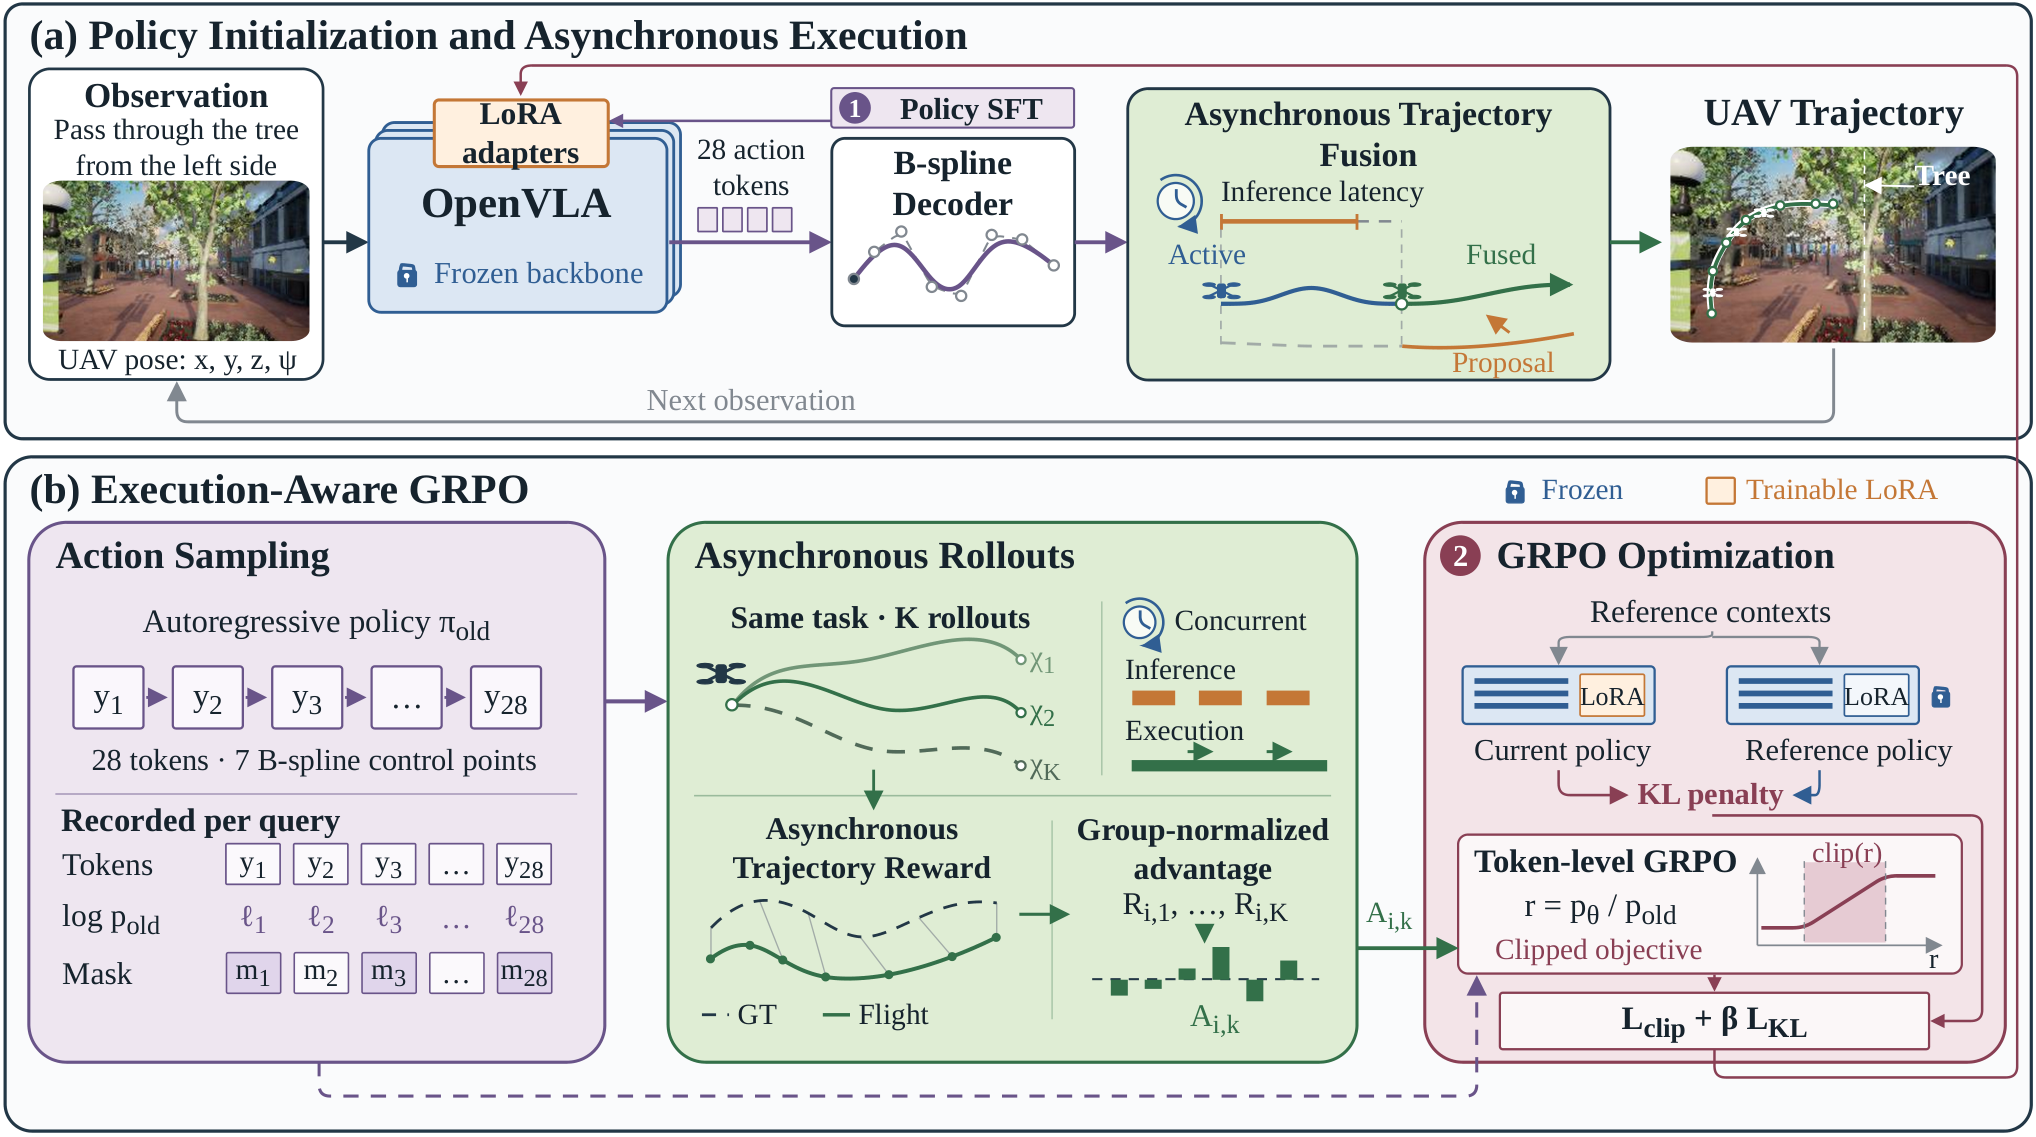
\includegraphics[width=\linewidth,height=26.5mm,keepaspectratio]{figures/p_aerodash.png}\par{\fontsize{6.6}{8}\selectfont\color{muted}AeroDASH · 2（论文原图）}\par\endgroup\vspace{1mm}

\noindent\begin{minipage}[t]{0.3233333333333333\linewidth}\vspace{0pt}\raggedright \par\ph{动作表示}\quad 28个token解码7\ensuremath{\times}4D控制点，加原点构成三次B样条；坐标锚在查询时的局部heading系。\par\vspace{0.7mm}
\end{minipage}\hfill
\begin{minipage}[t]{0.3233333333333333\linewidth}\vspace{0pt}\raggedright \par\ph{异步落地}\quad 返回时裁掉过期前缀，保留终点时间；按实际时间匹配位置／速度／加速度，而不是归一化参数。\par\vspace{0.7mm}
\end{minipage}\hfill
\begin{minipage}[t]{0.3233333333333333\linewidth}\vspace{0pt}\raggedright \par\ph{训练与结果}\quad 50k SFT后GRPO 2,730任务，LoRA r32；273条指令SR 76.56、nDTW .4495，无GRPO为56.41/\allowbreak{}.3913。\par\vspace{0.6mm}
\end{minipage}\par
\takeaway{架构核心：直接预测B样条控制点，按查询／切换时间对齐延迟提案，再匹配物理时间上的位置、速度与加速度。}

\note{AeroDASH以OpenVLA预测七个四维控制点，加固定原点形成三次B样条；SFT标签由专家短轨迹最小二乘拟合得到。在线将查询时的局部坐标转换到世界系，并按切换时间裁去延迟前缀，再以当前活动参考的平坦输出及前两阶导数作等式约束拟合剩余轨迹。GRPO以执行轨迹nDTW为奖励，仅训练LoRA。在273条语言任务上，样条SFT为56.41，GRPO后76.56；另用控制测试与实机案例展示轨迹连续性。}
\end{frame}
\gdef\slidesource{原文依据：\href{https://arxiv.org/html/2610.25407v1}{[24] AeroDASH}}
\begin{frame}[t,label=aero_curves]{AeroDASH：物理时间对齐与二阶连续交接}
\relax

\noindent\begin{minipage}[t]{0.55\linewidth}\vspace{0pt}\raggedright \par\begingroup\centering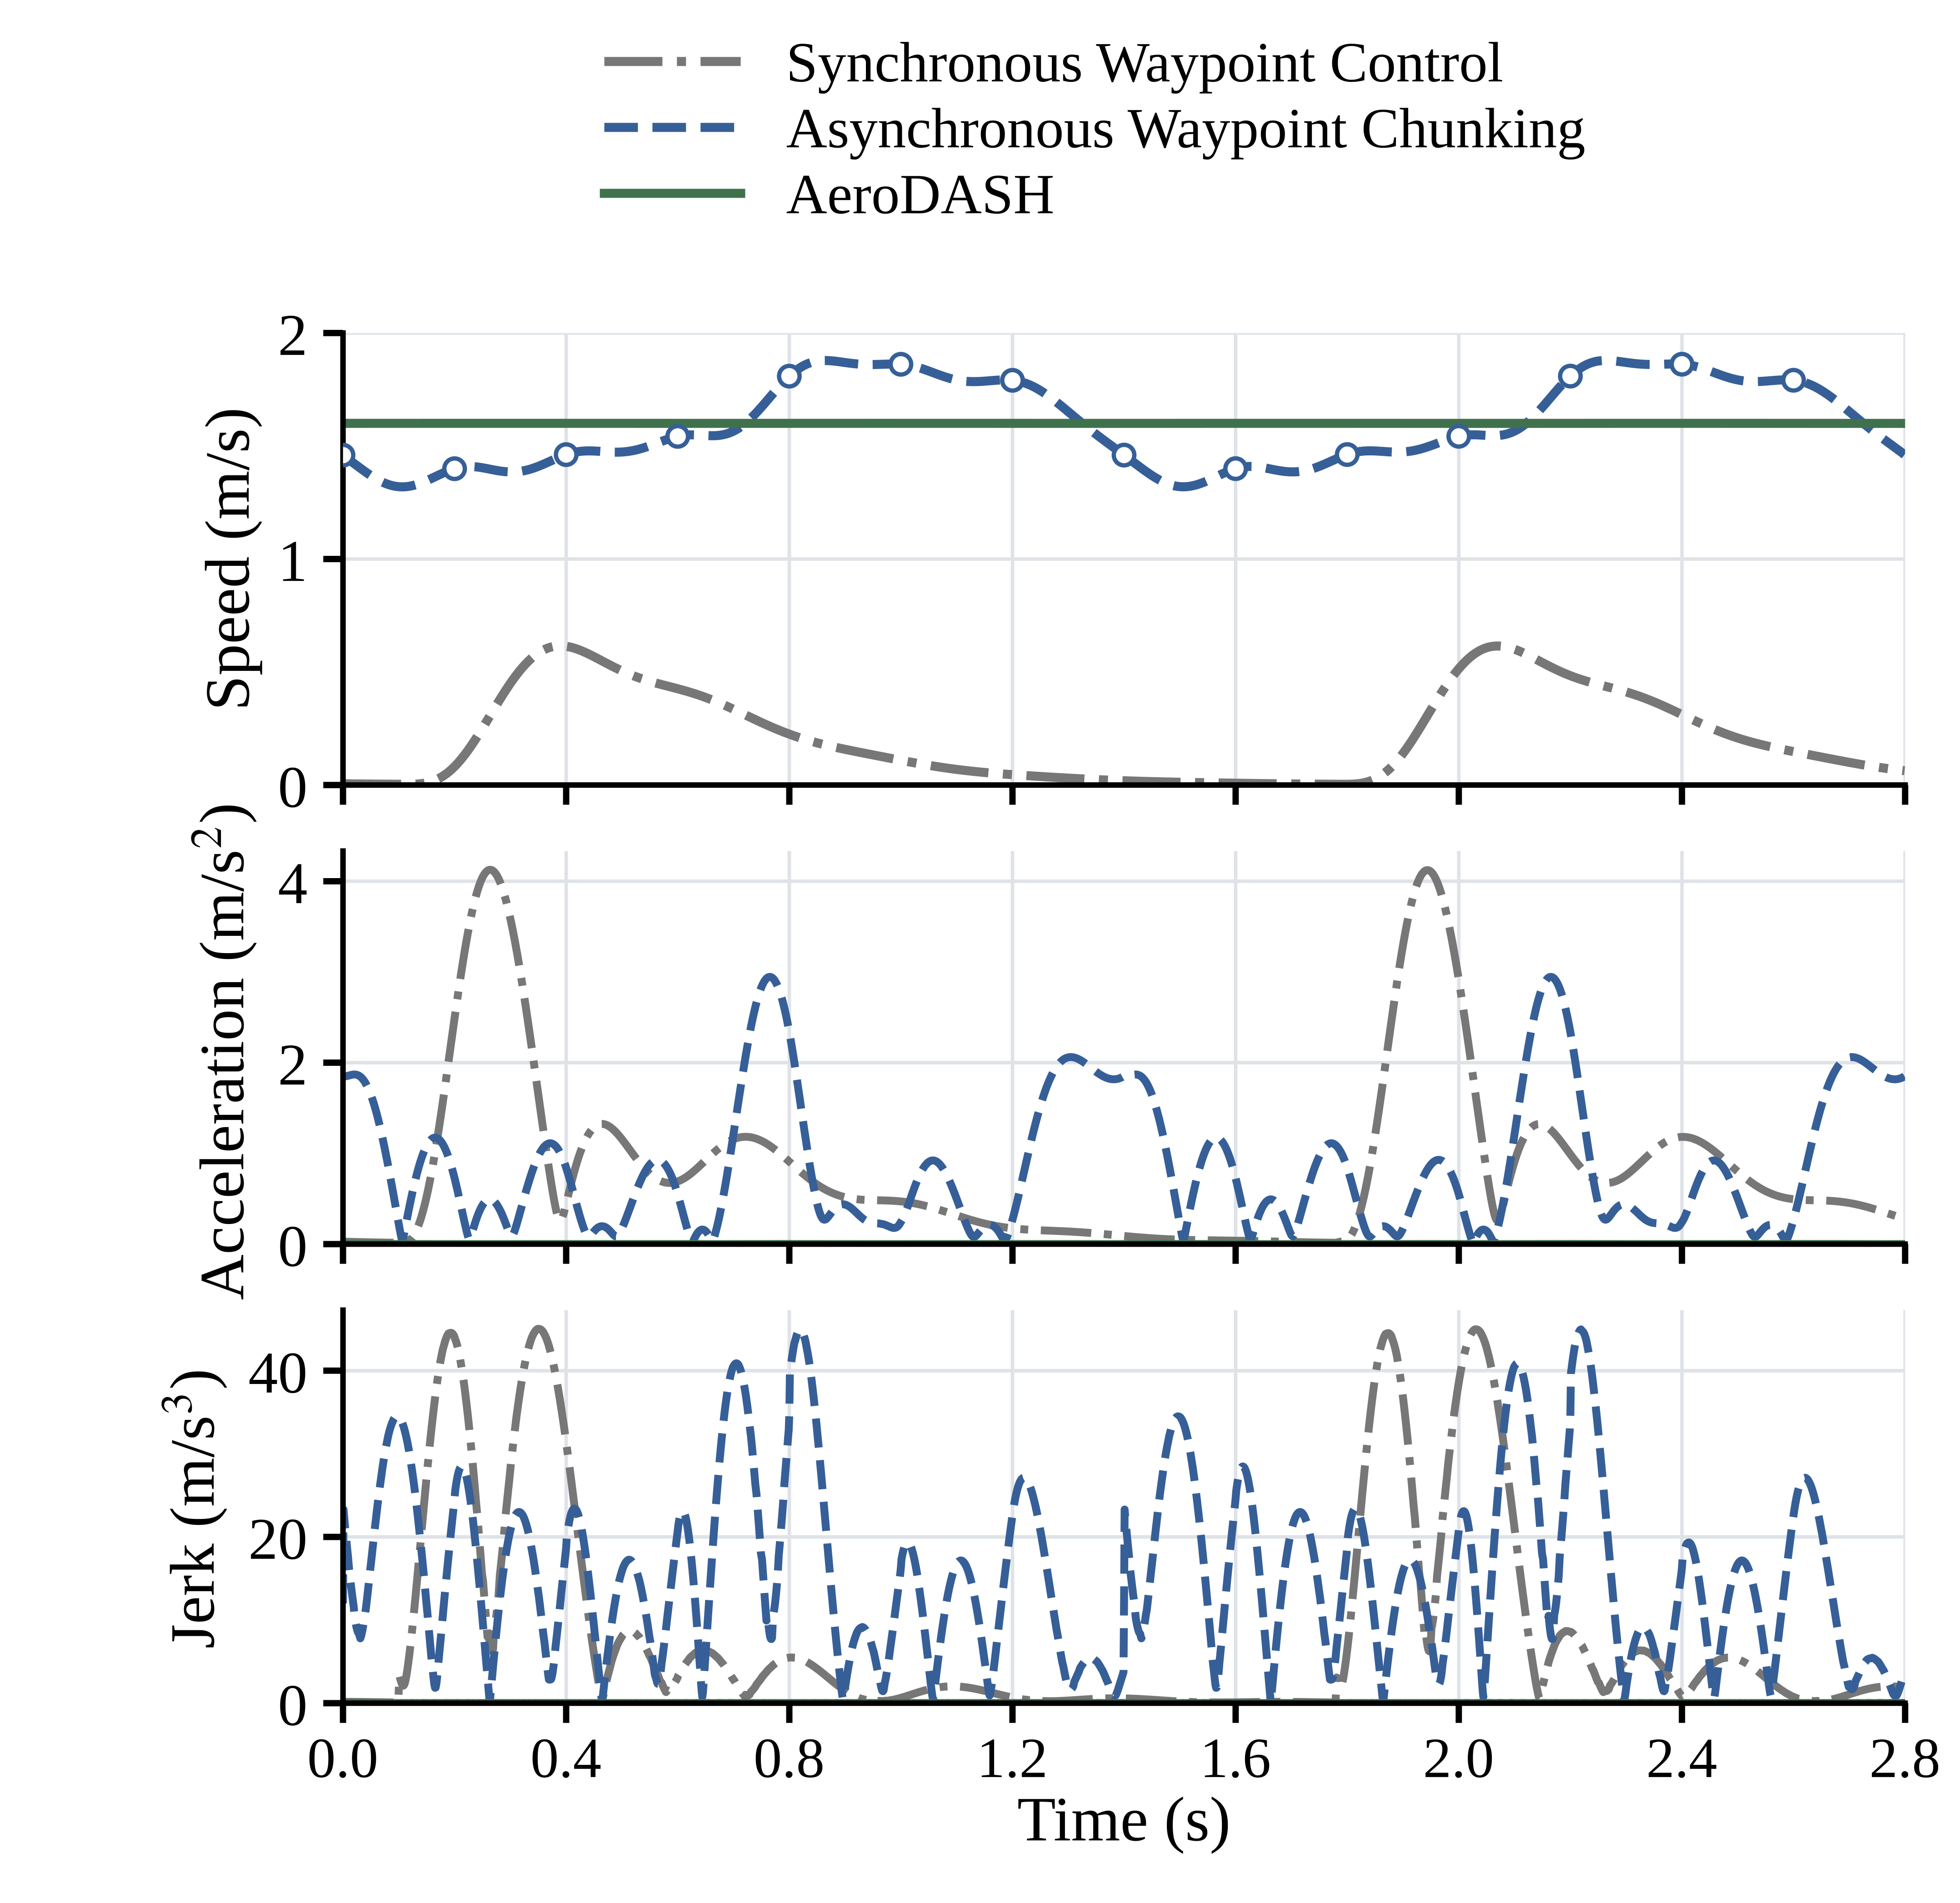
\includegraphics[width=\linewidth,height=33.0mm,keepaspectratio]{figures/p_aerodash_execution.png}\par{\fontsize{6.6}{8}\selectfont\color{muted}AeroDASH · Figure 5（论文原图）}\par\endgroup\vspace{1mm}
\end{minipage}\hfill
\begin{minipage}[t]{0.43\linewidth}\vspace{0pt}\raggedright \par\begingroup\centering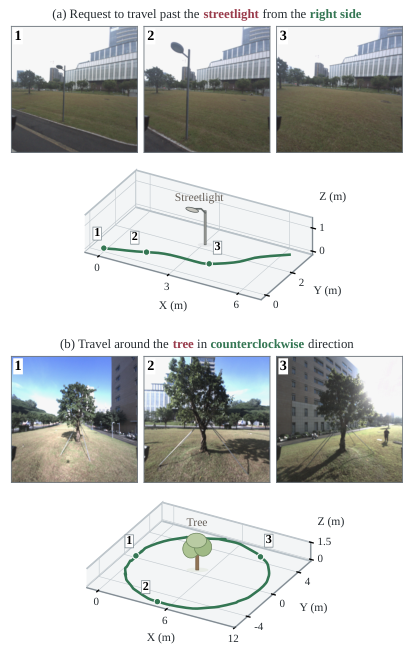
\includegraphics[width=\linewidth,height=33.0mm,keepaspectratio]{figures/p_aerodash_real.png}\par{\fontsize{6.6}{8}\selectfont\color{muted}AeroDASH · Figure 6（论文原图）}\par\endgroup\vspace{1mm}
\end{minipage}\par
\[p_{\rm new}^{(r)}(t_s)=p_{\rm old}^{(r)}(t_s),\quad r=0,1,2;\qquad \frac{d^rp}{dt^r}=T^{-r}\frac{d^rq}{du^r}\]\par\ph{图在说什么}\quad 延迟提案先裁过期前缀并保留原结束时刻，再约束切换处的位置、速度、加速度；局部拟合抑制轨迹形变与jerk。\par\vspace{1mm}
\takeaway{表示、时序和学习相互配合：样条提供连续参考，时间融合修复延迟，GRPO优化闭环轨迹质量。}

\note{返回提案的前缀在无人机等待推理期间已过期，因此先取剩余时段并重新参数化，再解带等式边界约束的最小二乘问题。导数必须按剩余物理时长转换：一阶乘T的负一次、二阶乘T的负二次。新轨迹在切换时刻匹配当前活动参考的平坦输出及前两阶导数。轨迹形变损失惩罚偏离提案、位置三阶导与yaw二阶导。TableI在相同273条语言任务上给出SR38.46、48.72、56.41、76.56，分别对应原基线、航点分块、样条SFT与样条加GRPO。}
\end{frame}
\section{机器人运行与工具接口}
\gdef\slidesource{原文依据：\href{https://arxiv.org/html/2607.18060v3}{[29] RoboHarness（编排）}}
\begin{frame}[t,label=harness_overview]{RoboHarness：保留原生策略，显式管理接管}
\relax
\par\begingroup\centering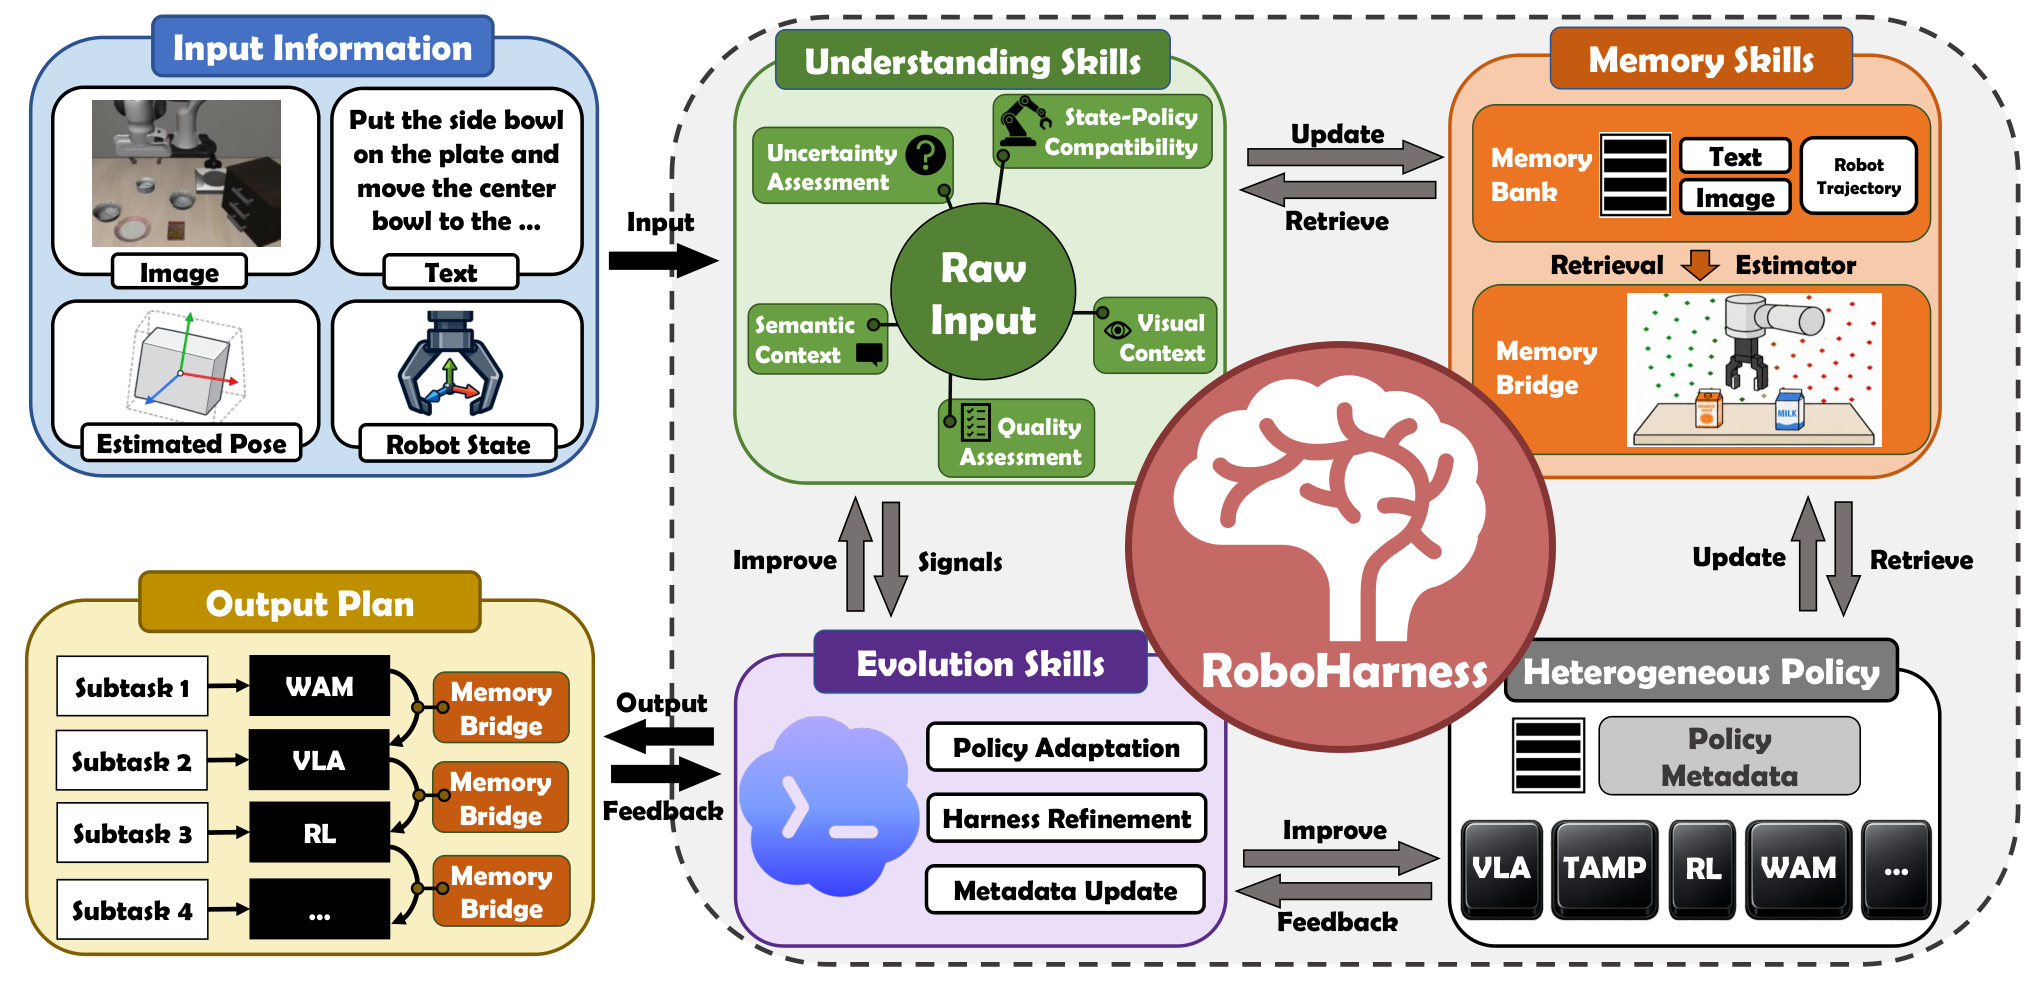
\includegraphics[width=\linewidth,height=30.0mm,keepaspectratio]{figures/p_roboharness_memory.png}\par{\fontsize{6.6}{8}\selectfont\color{muted}RoboHarness（编排） · Figure 1（论文原图）}\par\endgroup\vspace{1mm}

\noindent\begin{minipage}[t]{0.3233333333333333\linewidth}\vspace{0pt}\raggedright \par\ph{策略编排}\quad 能力卡保留VLA/\allowbreak{}WAM/\allowbreak{}RL/\allowbreak{}TAMP的原生接口；harness读当前任务和场景，按经验选下一个策略。\par\vspace{1mm}
\end{minipage}\hfill
\begin{minipage}[t]{0.3233333333333333\linewidth}\vspace{0pt}\raggedright \par\ph{状态交接}\quad 不是换个提示就接管；Memory Bridge先找“有成功经验且当前可达”的状态，再做桥接。\par\vspace{1mm}
\end{minipage}\hfill
\begin{minipage}[t]{0.3233333333333333\linewidth}\vspace{0pt}\raggedright \par\ph{实验范围}\quad v3在LIBERO-LoHo和消融里用了Faster-WAM；其他基准使用\ensuremath{\pi}0.5＋TAMP，按任务配置互补策略。\par\vspace{1mm}
\end{minipage}\par
\takeaway{方法要点：策略保留原生接口，harness利用能力描述、成功记忆和执行日志决定分解、路由与接管。}

\note{编排型RoboHarness用coding agent组织理解、记忆和演化三类技能。理解层读取图像质量、物体位姿稳定性、文本和视觉经验相似性以及状态兼容性，判断哪个策略适合当前子任务；记忆层为每个策略保存成功轨迹，为全部交互保存执行日志；演化层利用结果调整策略与编排方式。策略可为VLA、WAM、RL和TAMP，保留各自输入输出。v3的LIBERO-LoHo与异构消融包含Faster-WAM。它的贡献是动态能力判断和状态分布交接，后页说明Memory Bridge怎样实现。}
\end{frame}
\gdef\slidesource{原文依据：\href{https://arxiv.org/html/2607.18060v3}{[29] RoboHarness（编排）}}
\begin{frame}[t,label=harness_bridge]{Memory Bridge：交接进入经验支持邻域}
\relax
\par\begingroup\centering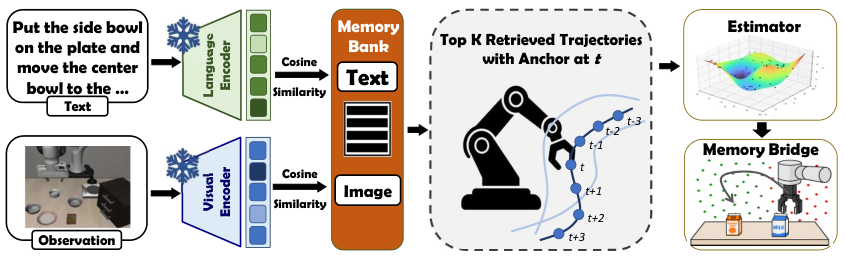
\includegraphics[width=\linewidth,height=17.5mm,keepaspectratio]{figures/harness_memory_bridge.png}\par{\fontsize{6.6}{8}\selectfont\color{muted}RoboHarness（编排） · Figure 2（论文原图）}\par\endgroup\vspace{1mm}

\noindent\begin{minipage}[t]{0.3233333333333333\linewidth}\vspace{0pt}\raggedright \par\ph{检索与排序}\quad 先文本、再视觉检索下一子任务的成败轨迹；锚附近用带符号时间偏移训练ranking SVM，估局部前向进度。\par\vspace{1mm}
\end{minipage}\hfill
\begin{minipage}[t]{0.3233333333333333\linewidth}\vspace{0pt}\raggedright \par\ph{约束接管}\quad 在记忆支持邻域和运动可达域的交集里，平衡进度与运动代价；到达后再核对对象、任务和场景。\par\vspace{1mm}
\end{minipage}\hfill
\begin{minipage}[t]{0.3233333333333333\linewidth}\vspace{0pt}\raggedright \par\ph{结果与条件}\quad LoHo平均PS/\allowbreak{}SR 98.2/\allowbreak{}96.0；Plus 91.9 vs \ensuremath{\pi}0.5 85.7，但后者表只有\ensuremath{\pi}0.5＋TAMP；记忆可跨同任务trial累积。\par\vspace{1mm}
\end{minipage}\par
\[\max_{s\in\mathcal R_{\rm conf}\cap\mathcal S_{\rm plan}} f_{\rm progress}(s)-\lambda C_{\rm motion}(s_t,s),\quad f_{\rm progress}(s)\geq\theta\]\takeaway{交接目标同时满足三项条件：下一策略有相近成功经验、局部任务进度足够、当前运动规划可以到达。}

\note{Memory Bridge先按文本检索再按视觉检索下一策略的成功轨迹锚点，在同一子任务内收集锚点前后状态，以带符号的时间偏移训练局部ranking SVM。候选接管状态限定在记忆状态的邻域及可达域交集中，最大化局部前向进度减运动成本，再由规划器生成桥接动作。到达后重新检查任务、对象与观察条件，完成接管。经验可在同任务多trial间积累；96.0为LoHo成功率，91.9为Plus结果。局部排序的作用是选择更易接管的状态。}
\end{frame}
\gdef\slidesource{原文依据：\href{https://arxiv.org/html/2610.14018v2}{[30] RoboHarness（几何）}}
\begin{frame}[t,label=harness_geometry]{几何型RoboHarness：工具调用落到可验证状态}
\relax

\noindent\begin{minipage}[t]{0.59\linewidth}\vspace{0pt}\raggedright \par\begingroup\centering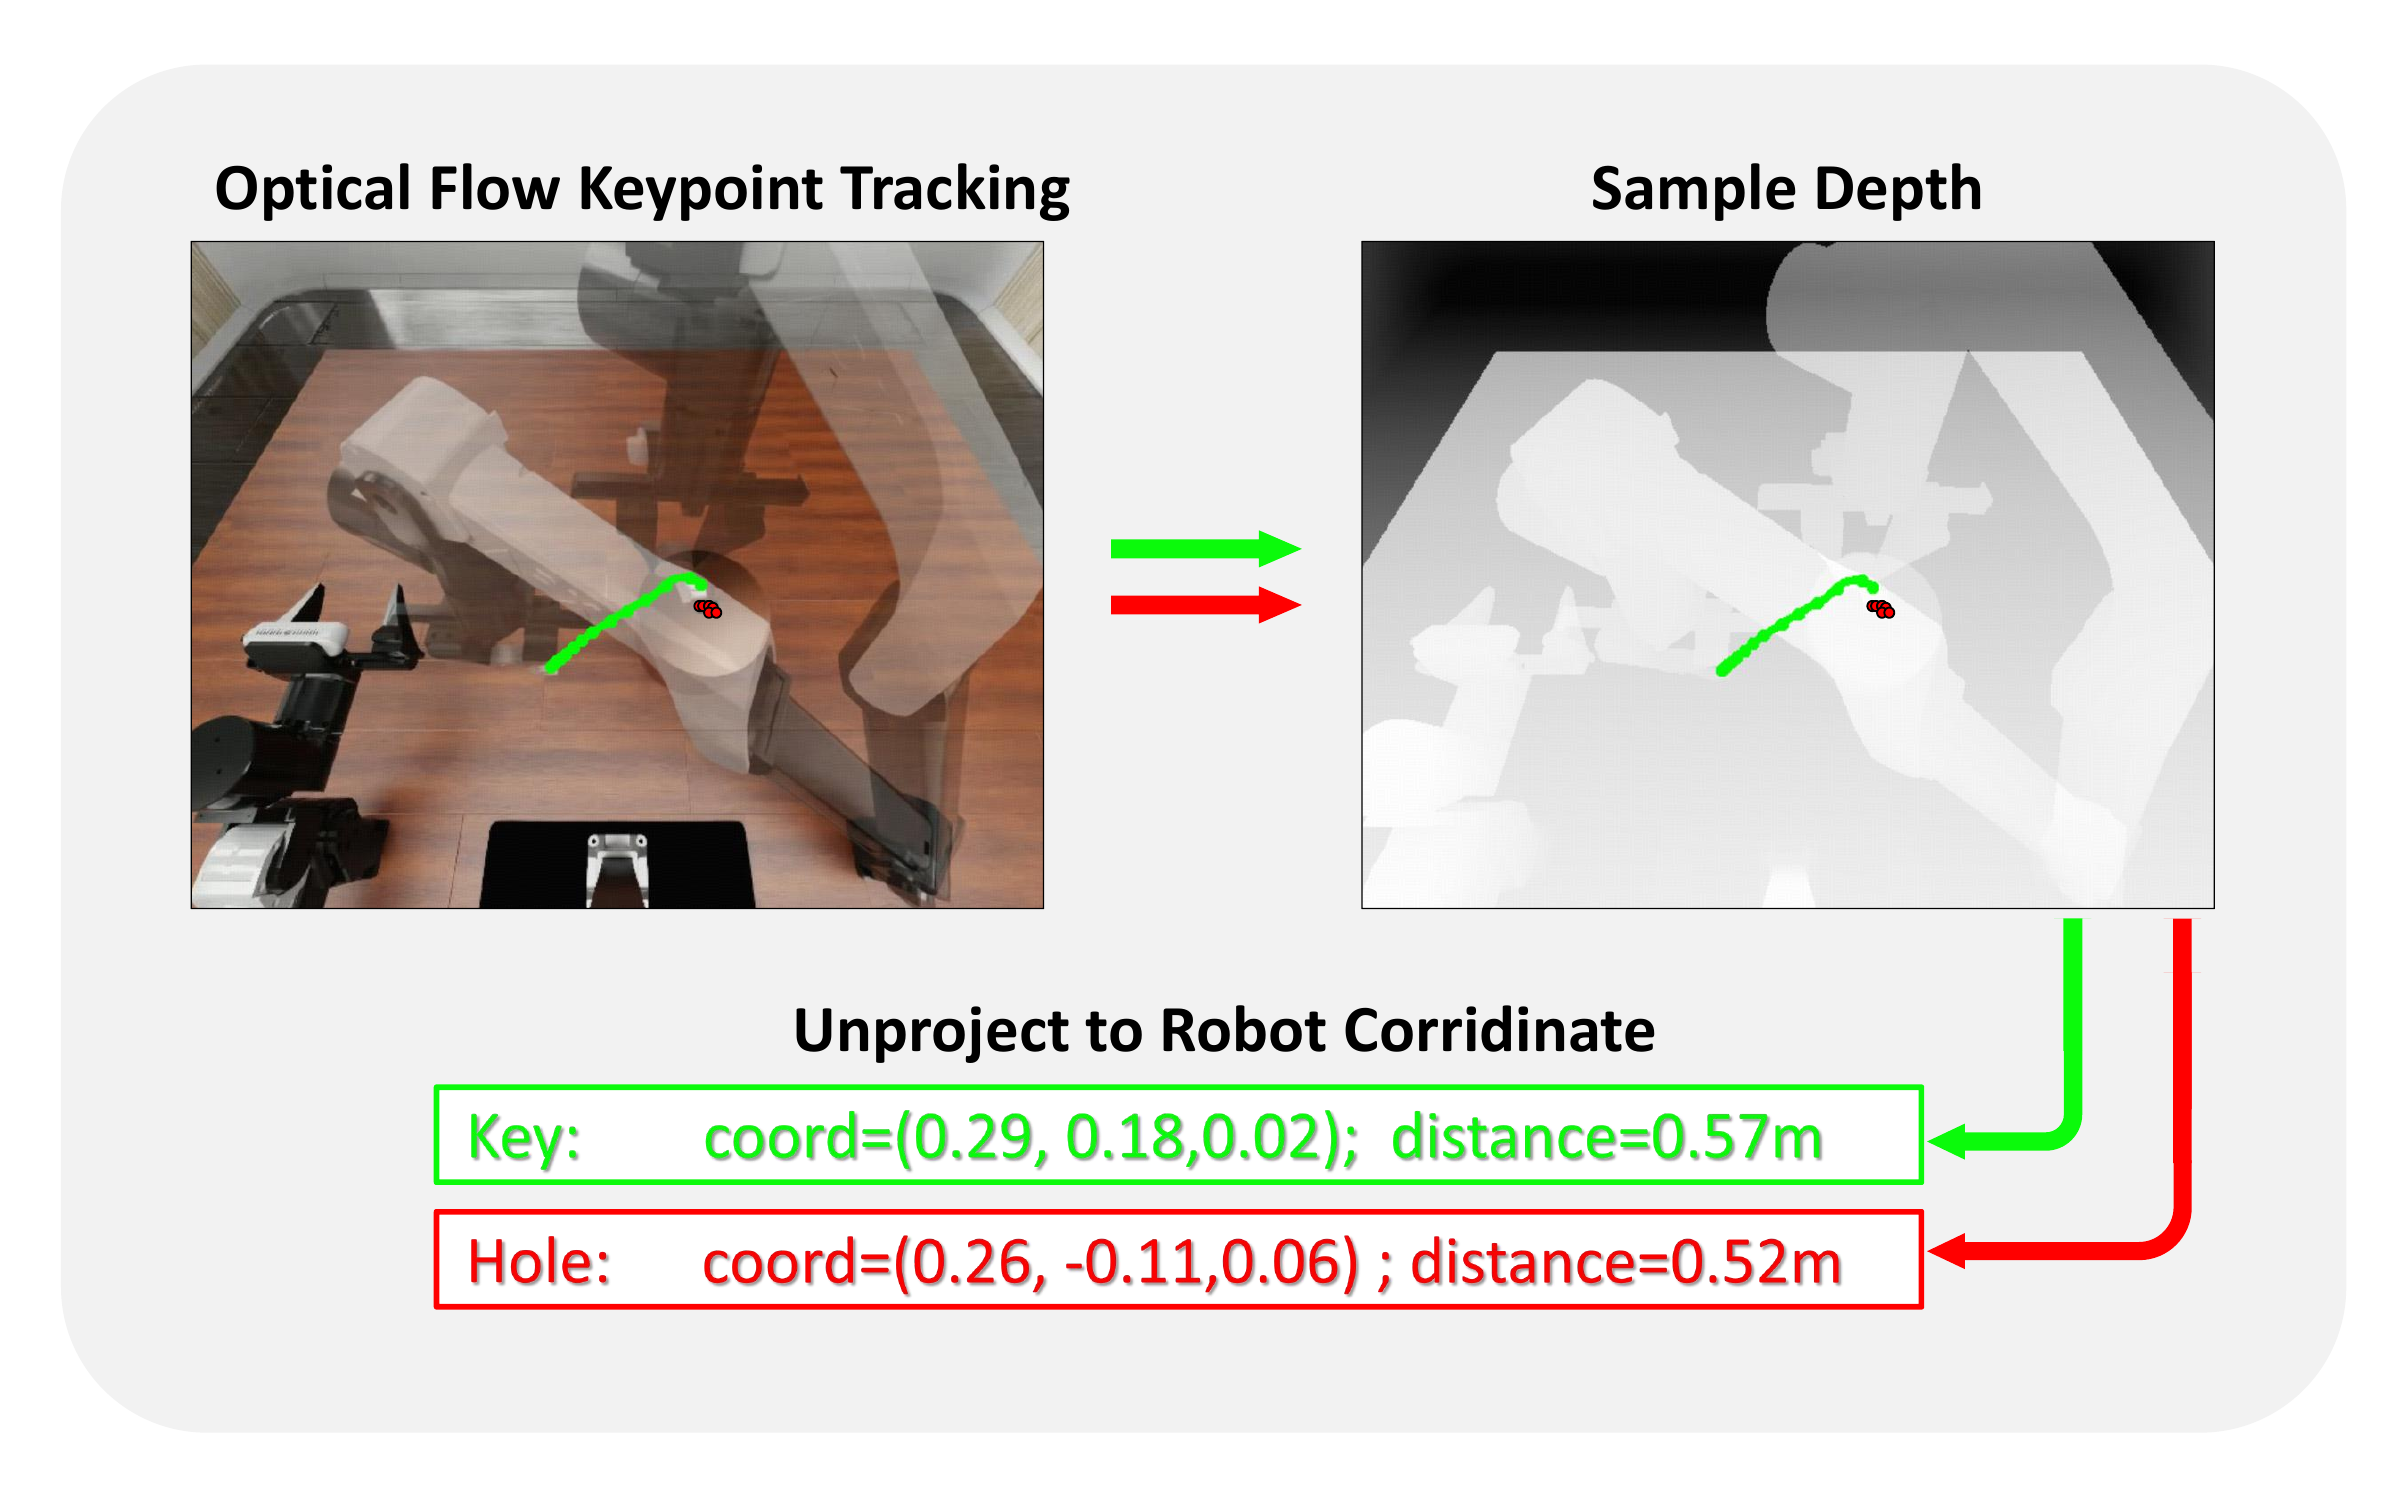
\includegraphics[width=\linewidth,height=30mm,keepaspectratio]{figures/harness_geometry_tracking.png}\par{\fontsize{6.6}{8}\selectfont\color{muted}RoboHarness（几何） · Figure 3（论文原图）}\par\endgroup\vspace{1mm}
\end{minipage}\hfill
\begin{minipage}[t]{0.39\linewidth}\vspace{0pt}\raggedright \par\begingroup\centering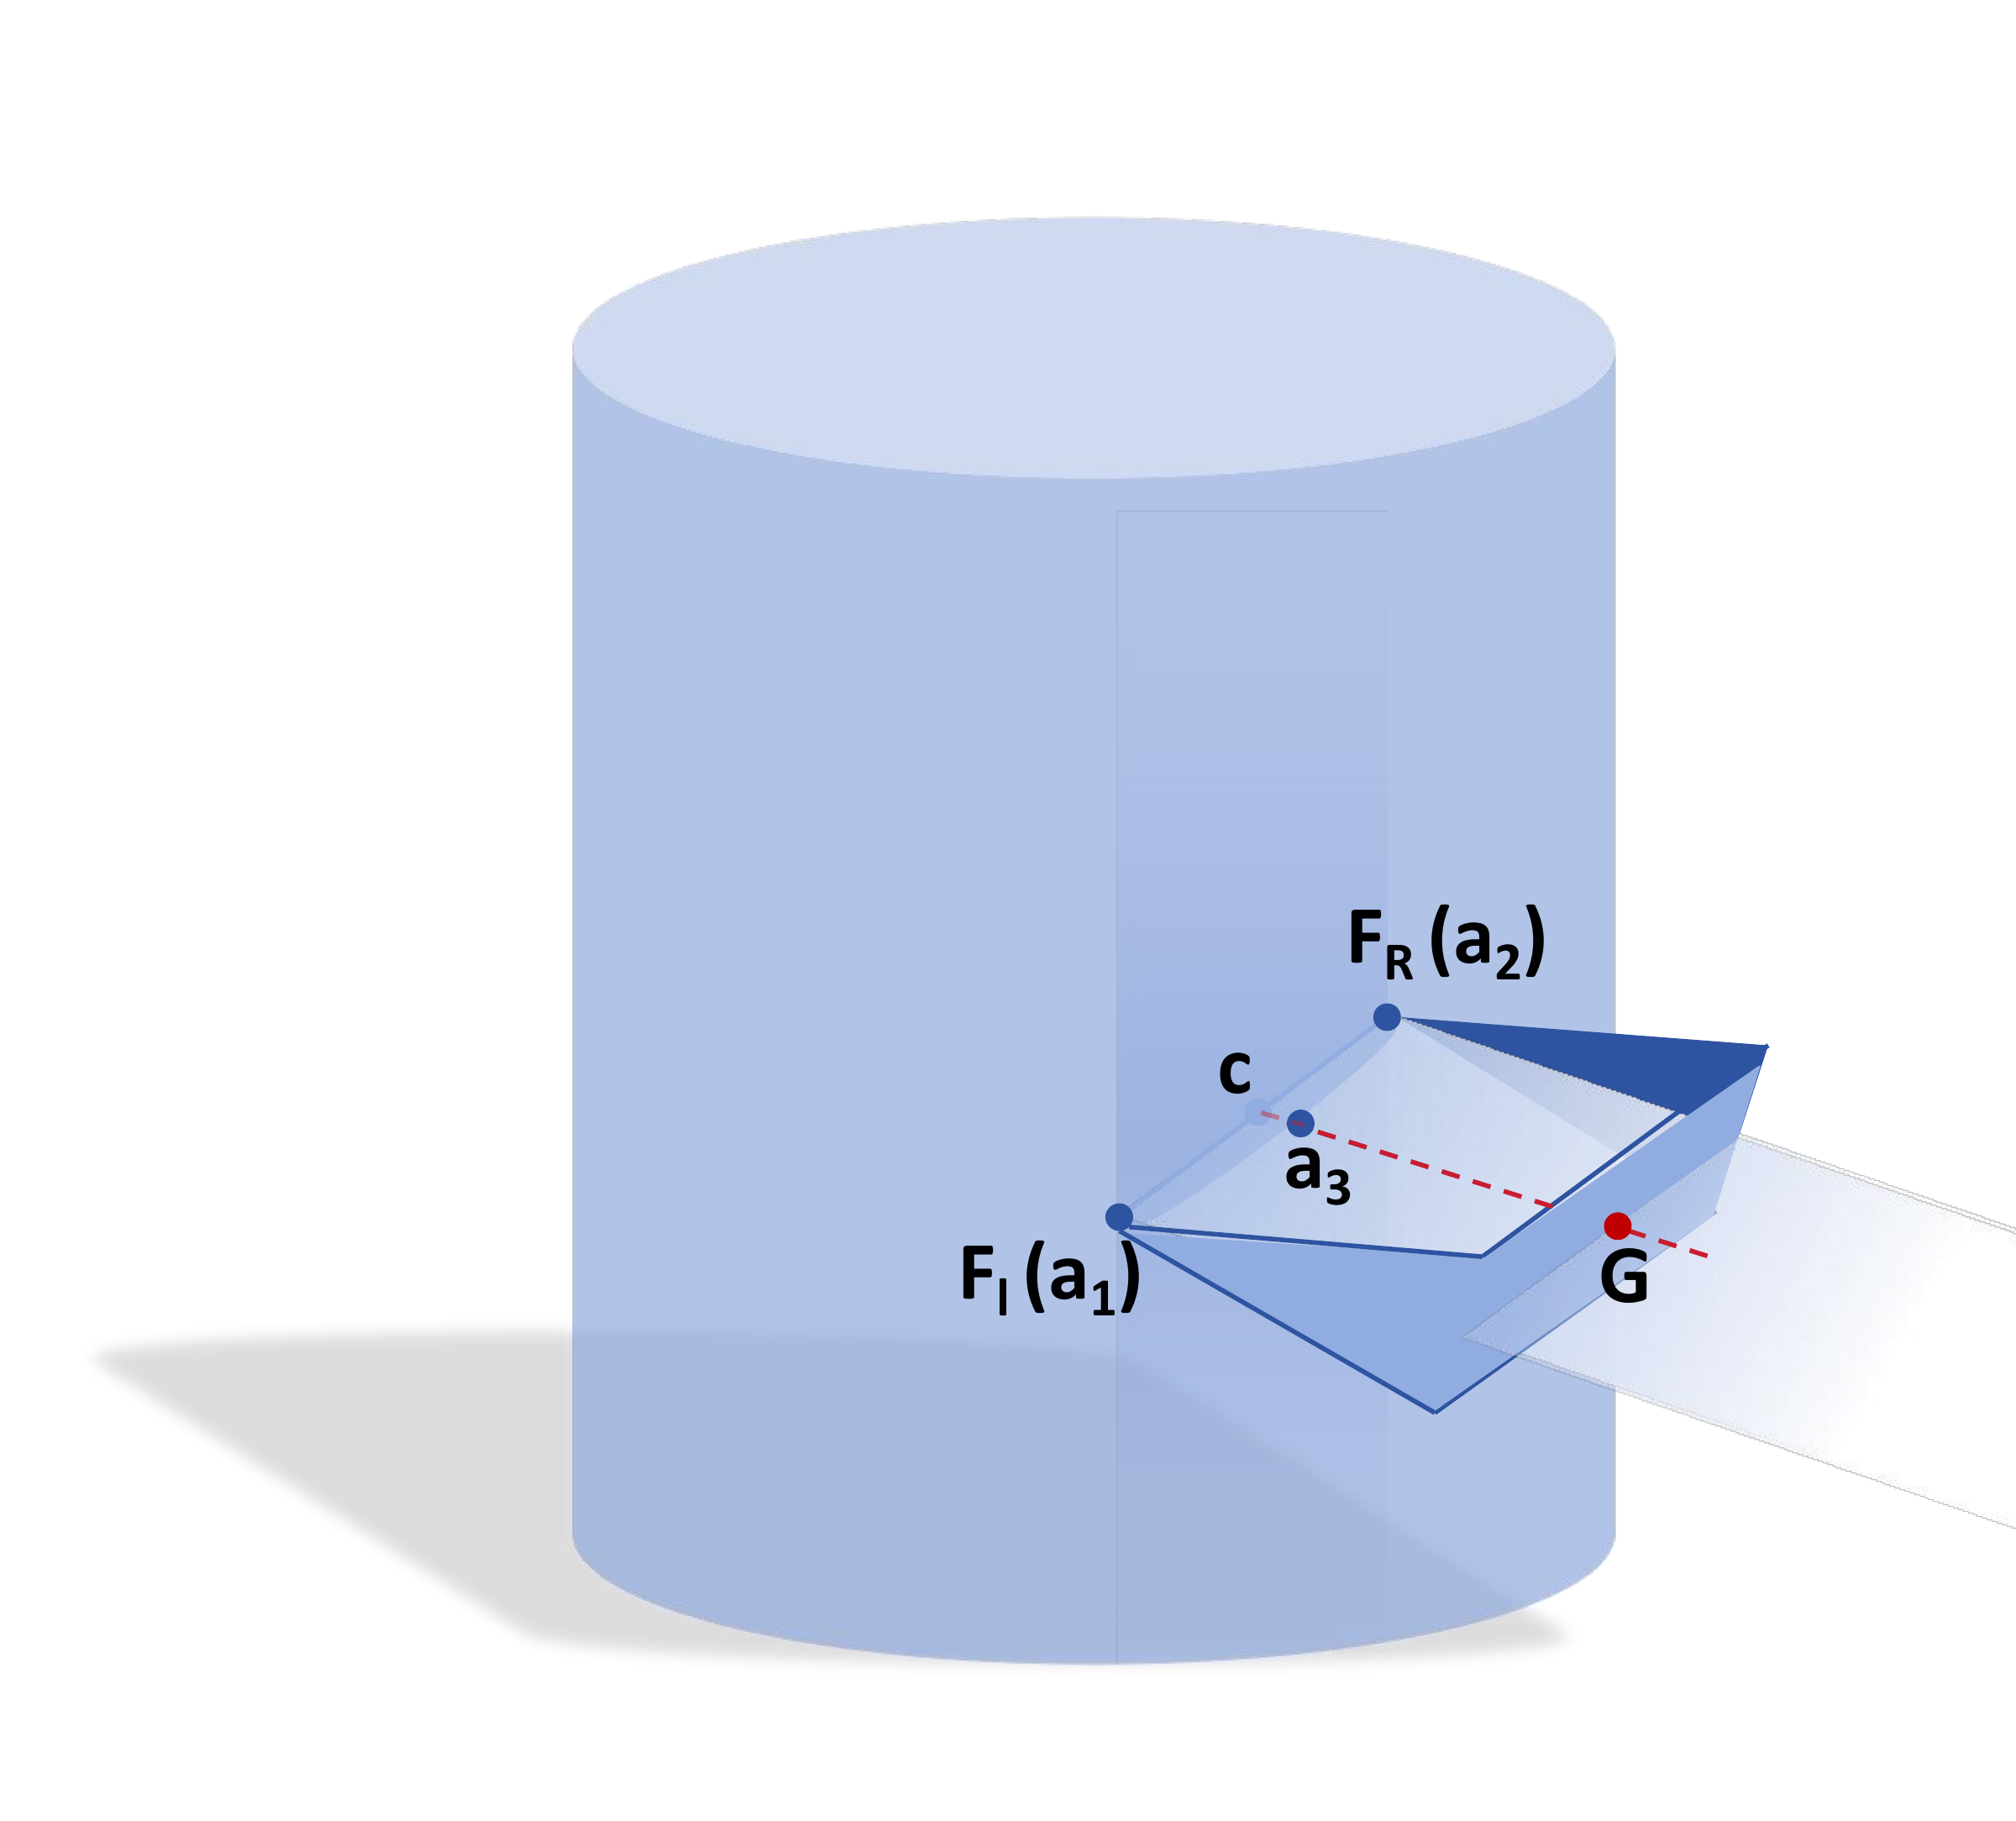
\includegraphics[width=\linewidth,height=30mm,keepaspectratio]{figures/harness_geometry_grasp_constraint.png}\par{\fontsize{6.6}{8}\selectfont\color{muted}RoboHarness（几何） · Figure 4（论文原图）}\par\endgroup\vspace{1mm}
\end{minipage}\par

\noindent\begin{minipage}[t]{0.3233333333333333\linewidth}\vspace{0pt}\raggedright \par\ph{状态接口}\quad LLM在图像里选关键点；光流跟踪、深度反投影到米制机器人坐标；遮挡或深度失效就重新检查。\par\vspace{1mm}
\end{minipage}\hfill
\begin{minipage}[t]{0.3233333333333333\linewidth}\vspace{0pt}\raggedright \par\ph{动作接口}\quad on-hand／off-hand关键点关系描述接触pose；几何关系满足后，还要过IK、规划、执行和复观测。\par\vspace{1mm}
\end{minipage}\hfill
\begin{minipage}[t]{0.3233333333333333\linewidth}\vspace{0pt}\raggedright \par\ph{实验}\quad BEHAVIOR前10个任务\ensuremath{\times}5次，q-score .44539（不是44.539\%完整SR）；每个任务有人工步骤。\par\vspace{1mm}
\end{minipage}\par
\takeaway{方法要点：让LLM选可见关键点和几何关系，将三维坐标恢复、约束求解、IK与运动规划交给工具。}

\note{几何型RoboHarness通过track_object维持LLM可读的米制关键点状态。图像选点后用光流跟踪，以深度反投影为相机坐标；执行工具接受on-hand与off-hand关键点关系，例如接触、共线、线垂直平面和平面平行。工具采样满足关系的目标姿态，筛IK可达性，再规划执行和重观测。BEHAVIOR十任务各五个实例，平均q-score0.44539；任务提示包含人工编写步骤。核心贡献在于以较小的几何工具集合连接通用语言推理与机器人动作。}
\end{frame}
\gdef\slidesource{\href{https://arxiv.org/html/2610.14018v2}{[30] RoboHarness（几何工具）} · §3.2；§4.1–4.2；Figs.4–5（统一变换记号）}
\begin{frame}[t,label=harness_geometry_math]{几何工具：用关键点约束表达接触与持物关系}
\relax
\bline{抓取前：接触姿态}{夹爪两指尖与物体接触点重合，第三个关键点约束夹爪方向；LLM只需指定点和关系，由求解器搜索姿态。}
\bline{抓取后：刚体关系}{物体与夹爪形成固定相对变换；给定物体期望位姿，可反求末端执行器的目标位姿，再交由IK和轨迹规划。}\[T^w_{o}=T^w_{e}T^e_{o},\qquad T^{w,*}_{e}=T^{w,*}_{o}(T^e_{o})^{-1}\]\bline{反馈闭环}{工具返回关键点当前位置与执行结果，关系不满足时重新选点或做小幅姿态调整，避免语言模型直接猜测连续动作。}\takeaway{可复用思想：用具有几何含义的状态与操作原语，替代高层模型对每一步坐标和关节动作的直接生成。}
\note{本页公式以统一SE(3)记号解释论文的持物关系，e为末端执行器，o为持物，w为世界坐标。物体刚性固定于夹爪时，物体目标位姿与固定夹持变换共同确定末端目标。论文给出以关键点关系表达接触和持物姿态的表示性讨论；工程中IK、碰撞、物体滑移和感知误差仍由具体工具与反馈处理。这种接口思想适合迁移到无人机的目标朝向、视域和距离等观察约束。}
\end{frame}
\section{群体协作方法}
\gdef\slidesource{文献分析：\href{https://arxiv.org/html/2606.14772v1}{[12] ScoutVLA}；\href{https://arxiv.org/html/2601.07558v1}{[14] FlyCo}；\href{https://arxiv.org/html/2610.25407v1}{[24] AeroDASH}；\href{https://arxiv.org/html/2607.18060v3}{[29] RoboHarness（编排）}}
\begin{frame}[t,label=single_to_group]{单体研究留下四个可复用接口}
\relax
{\fontsize{8.7}{11.1}\selectfont
\rowcolors{2}{white}{zebra}
\begin{tabularx}{\linewidth}{@{}Y{0.48}Y{1.53}Y{0.99}@{}}\toprule
\rowcolor{navy}\thd{接口} & \thd{单体文献给的} & \thd{群体还要补的}\\\midrule
证据 & AirHunt确认；Scout固定回答器；RAVEN空间精度 & 对象关联、来源相关、反证撤销\\
观察 & Scout问题取景；FlyCo新增表面 & 在队友已选视角后算互补价值\\
预测 & ANWM候选未来；ForeFly／WorldVLN任务表征 & 明确反事实权限，验证任务价值\\
执行 & AeroDASH时间接轨；两篇harness工具／交接 & 观察合同、时限、中断、拒绝、真实返回\\
\bottomrule\end{tabularx}\par}
\par\ph{技术演进}\quad 从保存历史，到选择新视角，再到预测／执行闭环；群体层协调“缺什么证据”，单体层保留原生模型和控制。\par\vspace{1mm}
\par\ph{从单机到群体}\quad 共同任务需要把各机已有技能组织成互补观察：按属性缺口分工，按来源与时效融合，再根据新观察更新决策。\par\vspace{1mm}
\takeaway{单体模块已能维护地图、调整视角、预测运动与管理执行；群体层进一步协调观察资源与任务分工。}

\note{这一页收束单体部分，避免直接跳到多智能体。现有文献已经给出可用的模块基础，但接口语义并不相同。证据有远射线与近定位，动作有航点和样条，世界模型有不同条件权限，执行又有不同延迟和中断方式。因此后半部分的研究单位应是具备条件、代价和反馈的观察任务，而不是交换所有模型内部latent或原始动作token。}
\end{frame}
\gdef\slidesource{\href{https://arxiv.org/html/2505.09108v1}{[11] Air-Ground} · §3–6；Figs.2–5；Tables 6–7}
\begin{frame}[t,label=airground]{Air-Ground：任务驱动的空中语义地图与地面验证}
\relax
\par\begingroup\centering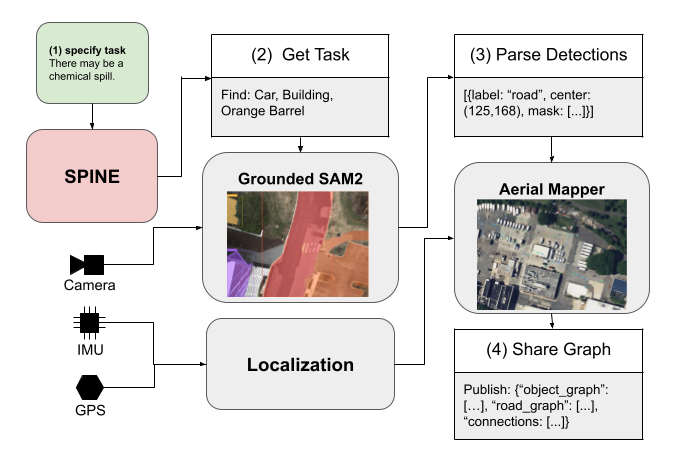
\includegraphics[width=\linewidth,height=28mm,keepaspectratio]{figures/p_airground.png}\par{\fontsize{6.6}{8}\selectfont\color{muted}Air-Ground Fig.3：UGV语义请求驱动UAV地图构建}\par\endgroup\vspace{1mm}

\noindent\begin{minipage}[t]{.323\linewidth}\vspace{0pt}\raggedright \ph{任务与共享状态}\quad UGV的SPINE把语言任务拆成语义类别请求；UAV以Grounded SAM2标道路和对象，构建可通行区域—对象图并共享。\par\end{minipage}\hfill\begin{minipage}[t]{.323\linewidth}\vspace{0pt}\raggedright \ph{执行与修正}\quad GNSS／IMU对齐跨机坐标，MOCHA机会通信传增量图；地面LiDAR和RGB-D补近景、删不可行边，LLM滚动调用行为库。\par\end{minipage}\hfill\begin{minipage}[t]{.323\linewidth}\vspace{0pt}\raggedright \ph{实机发现}\quad 团队控制任务5/6完成；无空中图UGV为0/3，GT图3/3。两次长任务约90/93\%自主运行，包含21/19次人工交互。\par\end{minipage}
\takeaway{方法要点：空中视角提供全局可通行先验，地面近景验证局部可行性，并把修正返回共享任务地图。}
\note{UAV根据地面任务请求改变检测类别，提取road区域和目标对象，以地区节点连接可通行空间，以对象边表示可观测关系。俯视图以GNSS和姿态投到共同UTM坐标。地面端维护占据图、语义对象和VLM描述，并通过add/remove nodes、add/remove edges和update_nodes向SPINE提供增量更新。SPINE规划导航、主动建图与人机交互行为，并验证可行性。MOCHA按链路条件交换图，UAV还能做消息中继。系统展示强调真实长任务、通信与地图修正；当前多个UGV之间没有另设协同分配。}
\end{frame}
\gdef\slidesource{原文依据：\href{https://arxiv.org/html/2603.12908v2}{[25] GoalSwarm}}
\begin{frame}[t,label=goalswarm]{GoalSwarm：共享语义值图与前沿成本竞拍}
\relax
{\fontsize{8.9}{11.0}\selectfont
\noindent\begin{minipage}[t]{0.58\linewidth}\vspace{0pt}\raggedright \par\begingroup\centering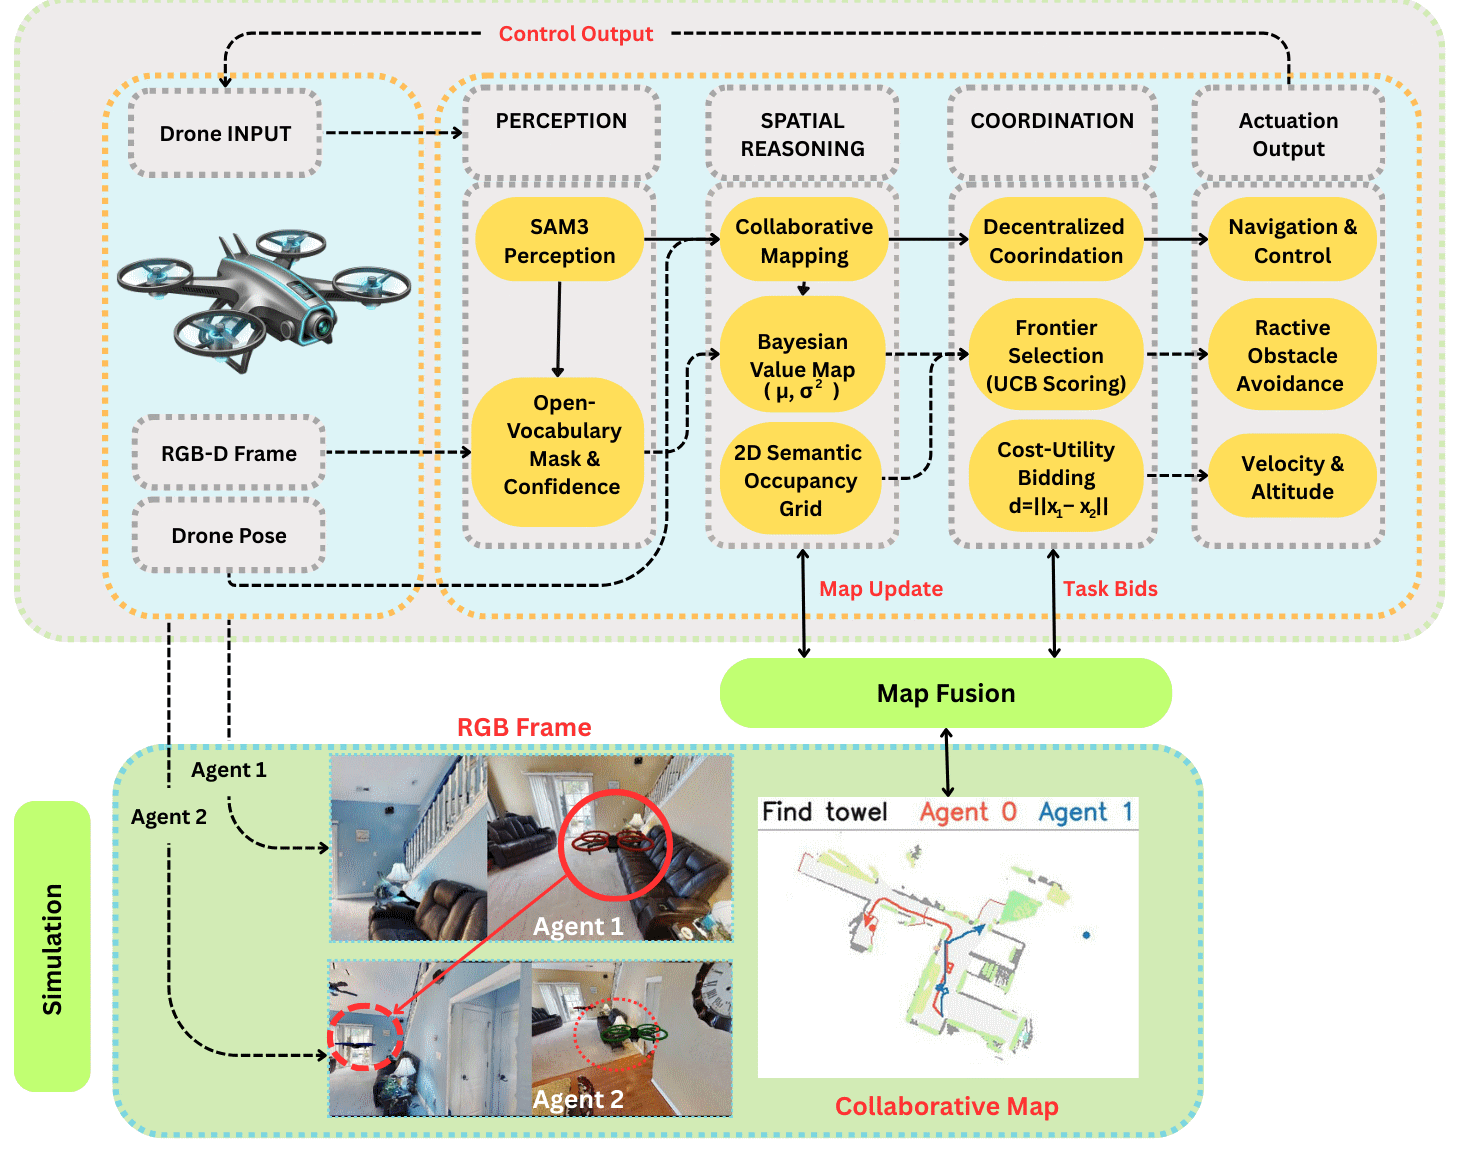
\includegraphics[width=\linewidth,height=30mm,keepaspectratio,trim=0.000bp 100.329bp 0.000bp 0.000bp,clip]{figures/p_goalswarm.png}\par{\fontsize{6.6}{8}\selectfont\color{muted}GoalSwarm · 2（原图局部放大）}\par\endgroup\vspace{1mm}
\end{minipage}\hfill
\begin{minipage}[t]{0.4\linewidth}\vspace{0pt}\raggedright \par\ph{感知与调度}\quad SAM3语义图、共享2D地图和贝叶斯值图；UCB竞拍分工，FMM与深度避障执行。地图25步同步。\par\vspace{1mm}
\par\ph{数据与先验}\quad GOAT对象子任务，24m\ensuremath{\times}24m；值图$\mu_0=.5$、$\sigma_0^2=.5$，2帧连续检测；完美里程计和通信，三维目标压成二维。\par\vspace{1mm}
\end{minipage}\par
{\fontsize{7.8}{9.8}\selectfont
\renewcommand{\arraystretch}{1.06}
\rowcolors{2}{white}{zebra}
\begin{tabularx}{\linewidth}{@{}Y{0.69}Y{1.29}Y{1.02}@{}}\toprule
\rowcolor{navy}\thd{配置} & \thd{SR / SPL} & \thd{说明}\\\midrule
完整系统 & 45 / .179 & 共享图＋UCB竞拍＋贝叶斯值图，20个子任务\\
无共享图 & 40 / .130 & 同流程去掉共享地图\\
单体参考 & 10 / — & 只有10个子任务（2回合），分母不同\\
\bottomrule\end{tabularx}\par}
\takeaway{架构核心：用语义均值与不确定性产生探索效用，结合路程和空间分离为多机分配前沿。}
}
\note{GoalSwarm将SAM3目标检测置信通过RGB-D投影到共享二维图。每个值图单元保持均值与方差，融合新观测时按观测方差与已有方差加权更新；视轴角度和距离影响观测置信。前沿效用用均值加标准差的UCB，竞拍再扣FMM路程成本和队友距离惩罚并考虑前沿尺寸。广播目标冲突时高分者优先；目标连续两帧检测后切换接近。TableII共同条件下完整45\%、无共享40\%，SPL0.179与0.130。地图25步同步，实验使用精确里程计与通信。}
\end{frame}
\gdef\slidesource{\href{https://arxiv.org/html/2603.12908v2}{[25] GoalSwarm} · §III-C–III-E；Eqs.6–11（统一符号）}
\begin{frame}[t,label=goalswarm_math]{GoalSwarm：不确定性探索与多机冲突消解}
\relax
\[U(f)=\widetilde\mu_f+\beta\widetilde\sigma_f,\qquad s_{j,f}=w_1U(f)-w_2C(p_j,f)+w_3|f|-P_{\rm sep}\]\bline{语义值图}{观测置信融合到空间均值和方差；均值表示目标相关性，较大方差使尚不确定的区域保留探索机会。}
\bline{成本竞拍}{C为FMM估计的可达路程，前沿大小鼓励覆盖，空间分离项抑制机间聚集；同一前沿冲突由得分决定优先级。}
\bline{与普通覆盖的差别}{前沿不再只按最近距离选择，而同时受目标语义、观测不确定性和队友位置影响；共享图让探索进度跨机可见。}\takeaway{群体主动感知已有“语义效用＋代价＋避重复”的实现基础，下一步可将效用细化到共同任务的未决属性。}
\note{UCB中的均值与方差取前沿周围圆形区域的中位数，beta=1.7。成本效用分数中空间分离项为距离不足dmin时的惩罚。该机制主要解决共享地图上的搜索覆盖与冲突；若任务需要背面文字等属性，地图中目标相关分数不能直接表达该属性是否已获取。因此后续研究以目标属性和问题可回答性为观察效用，将GoalSwarm作为明确的强基线。}
\end{frame}
\gdef\slidesource{原文依据：\href{https://arxiv.org/html/2603.20804v2}{[26] Co-VLN}}
\begin{frame}[t,label=covln]{Co-VLN：在独立任务间共享已有拓扑记忆}
\relax
\par\begingroup\centering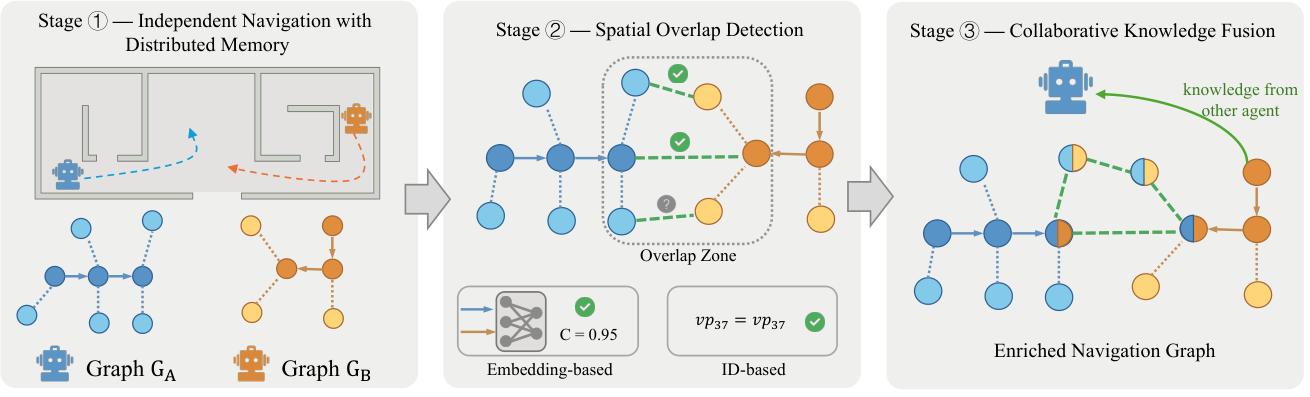
\includegraphics[width=\linewidth,height=21mm,keepaspectratio]{figures/p_covln.png}\par{\fontsize{6.6}{8}\selectfont\color{muted}Co-VLN · 2（论文原图）}\par\endgroup\vspace{1mm}

\noindent\begin{minipage}[t]{0.3233333333333333\linewidth}\vspace{0pt}\raggedright \par\ph{共享什么}\quad 各机有独立指令和目标；进入重叠空间后匹配拓扑节点、交换已有观测，后端可接DUET。\par\vspace{1mm}
\end{minipage}\hfill
\begin{minipage}[t]{0.3233333333333333\linewidth}\vspace{0pt}\raggedright \par\ph{学习与先验}\quad learned匹配按空间邻近标签训练；R2R val-unseen 2349条／11场景，默认2机；prior配对平均4.24个重叠视点，随机配对0.88。\par\vspace{1mm}
\end{minipage}\hfill
\begin{minipage}[t]{0.3233333333333333\linewidth}\vspace{0pt}\raggedright \par\ph{同配置效果}\quad DUET SR71.52\ensuremath{\to}74.50，SPL60.41\ensuremath{\to}62.56；oracle对应关系上界为76.23。\par\vspace{1mm}
\end{minipage}\par
\par\ph{与课题的关系}\quad 它证明队友的已有记忆能纠正导航；但还没有回答：共同任务缺属性时，该派谁去看新的地方。\par\vspace{1mm}
\takeaway{方法要点：匹配空间重叠节点，将队友的已探索拓扑与观察融合进自己的导航记忆。}

\note{各机独立导航并保存拓扑图，DUET节点为学习特征，MapGPT节点可为图像或文字描述。DUET的轻量Transformer匹配器学习两个节点是否在空间半径R内，而不是要求站在完全相同的离散视点；训练标签由训练场景位置构造。匹配置信再用于距离估计与知识融合，在导航记忆里扩充队友可达区域。DUET基线71.52提升到74.50，SPL60.41到62.56；oracle视点ID结果76.23作为对应关系上界。默认任务配对依据GT路线邻近先验以提高相遇机会。}
\end{frame}
\gdef\slidesource{原文依据：\href{https://arxiv.org/html/2603.20804v2}{[26] Co-VLN}}
\begin{frame}[t,label=covln_results]{Co-VLN：规模收益、重叠空间与路线纠正}
\relax

\noindent\begin{minipage}[t]{0.49\linewidth}\vspace{0pt}\raggedright \par\begingroup\centering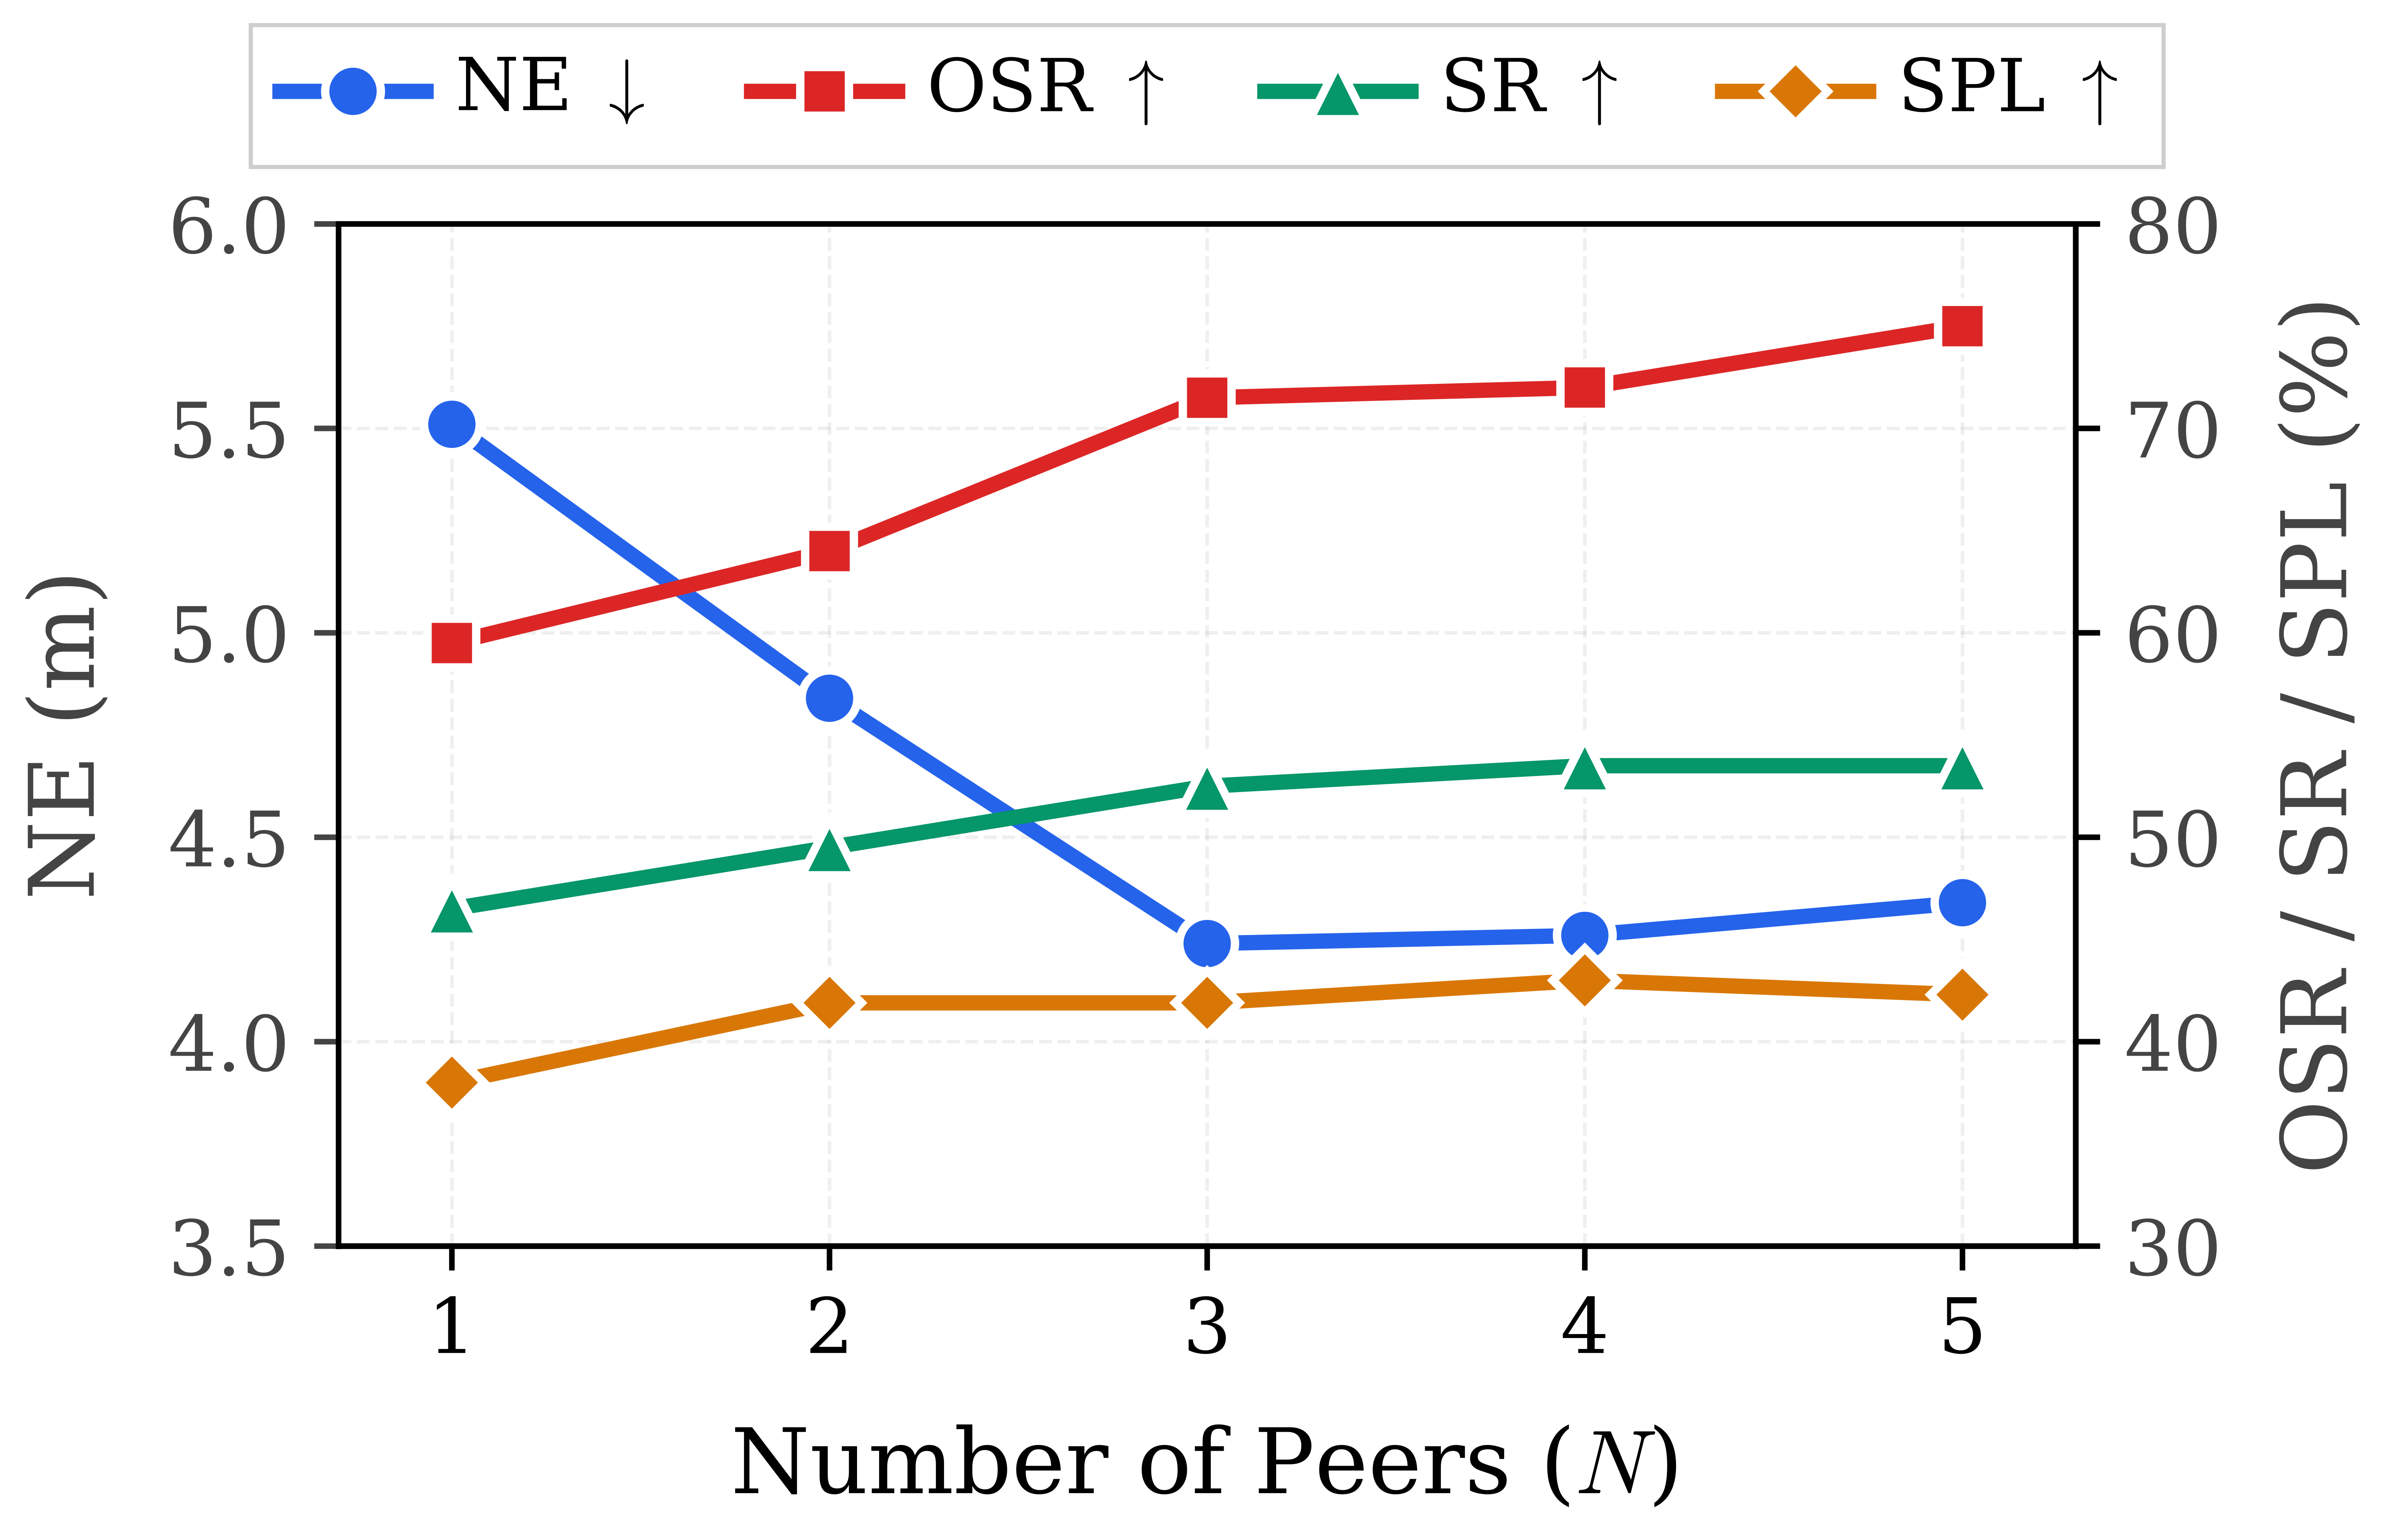
\includegraphics[width=\linewidth,height=33.5mm,keepaspectratio]{figures/p_covln_scaling.png}\par{\fontsize{6.6}{8}\selectfont\color{muted}Co-VLN · Figure 3（论文原图）}\par\endgroup\vspace{1mm}
\end{minipage}\hfill
\begin{minipage}[t]{0.49\linewidth}\vspace{0pt}\raggedright \par\begingroup\centering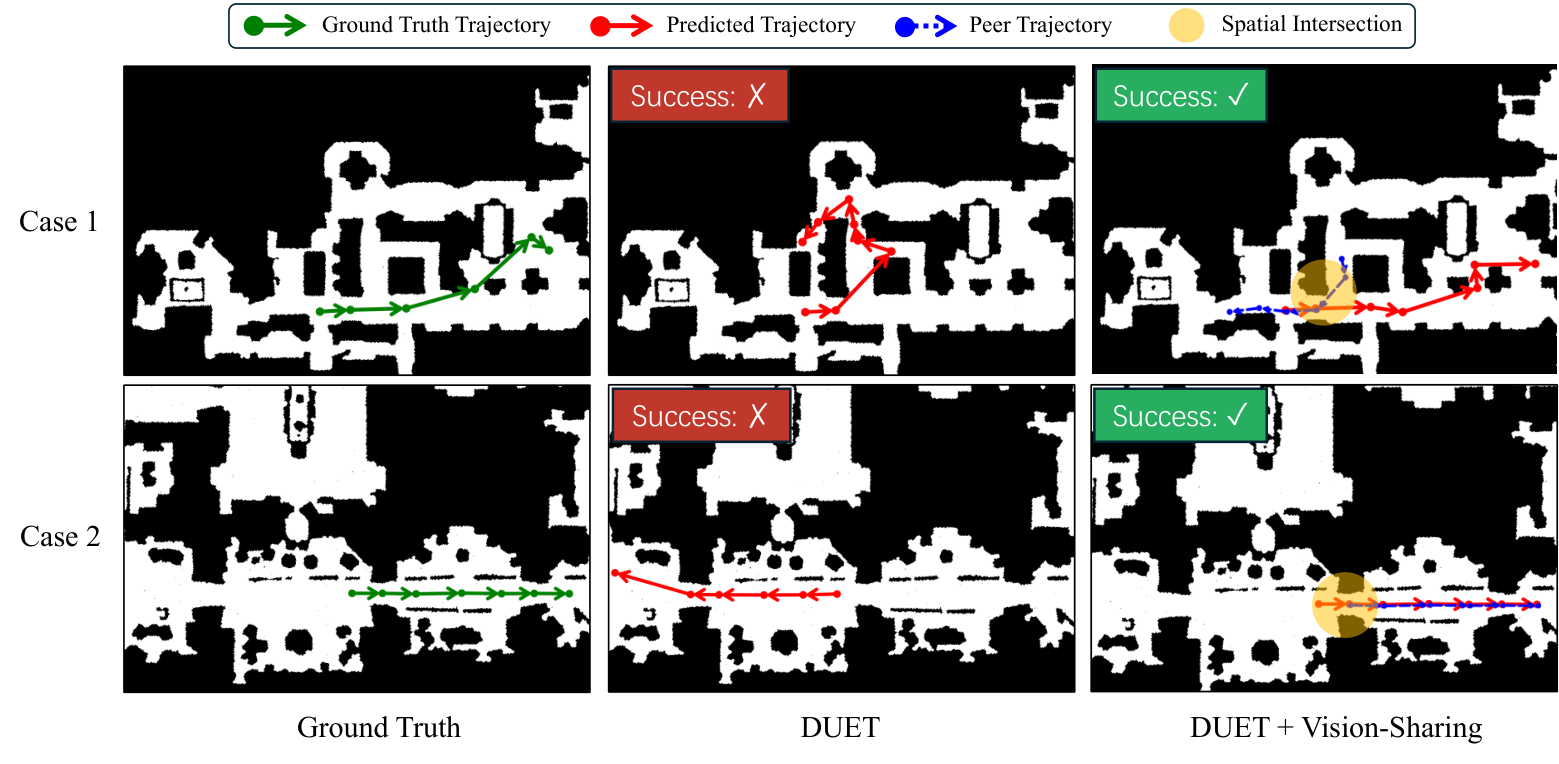
\includegraphics[width=\linewidth,height=33.5mm,keepaspectratio]{figures/p_covln_cases.png}\par{\fontsize{6.6}{8}\selectfont\color{muted}Co-VLN · Figure 4（论文原图）}\par\endgroup\vspace{1mm}
\end{minipage}\par
\par\ph{规模图}\quad 200条R2R-Hard主任务，每条选GT路径最大重叠的peer；收益随可共享拓扑增多而增长，并随重叠信息趋于重复而饱和。\par\vspace{1mm}
\par\ph{案例图}\quad 队友已经看过的节点帮助当前策略越过局部歧义并纠正路线；这种机制取决于重叠检测和共享区域的任务相关性。\par\vspace{1mm}
\takeaway{共享的价值取决于队友掌握了哪些自己缺少的环境信息，重叠检测决定这些信息能否正确接入。}

\note{Figure3在200条R2R-Hard主任务上选择路径重叠较多的peer，展示共享记忆随团队规模的收益；Figure4展示融合队友拓扑后修正路线的过程。它支持已有观察的复用，而进一步主动派遣队友去获取新的属性证据，需要增加观察分配机制。}
\end{frame}
\gdef\slidesource{\href{https://arxiv.org/html/2606.25119v1}{[27] SurveilNav} · §III–V；Figs.3–4；Tables I–IV}
\begin{frame}[t,label=surveilnav]{SurveilNav：固定外部视角与机载观察联合建图}
\relax
\par\begingroup\centering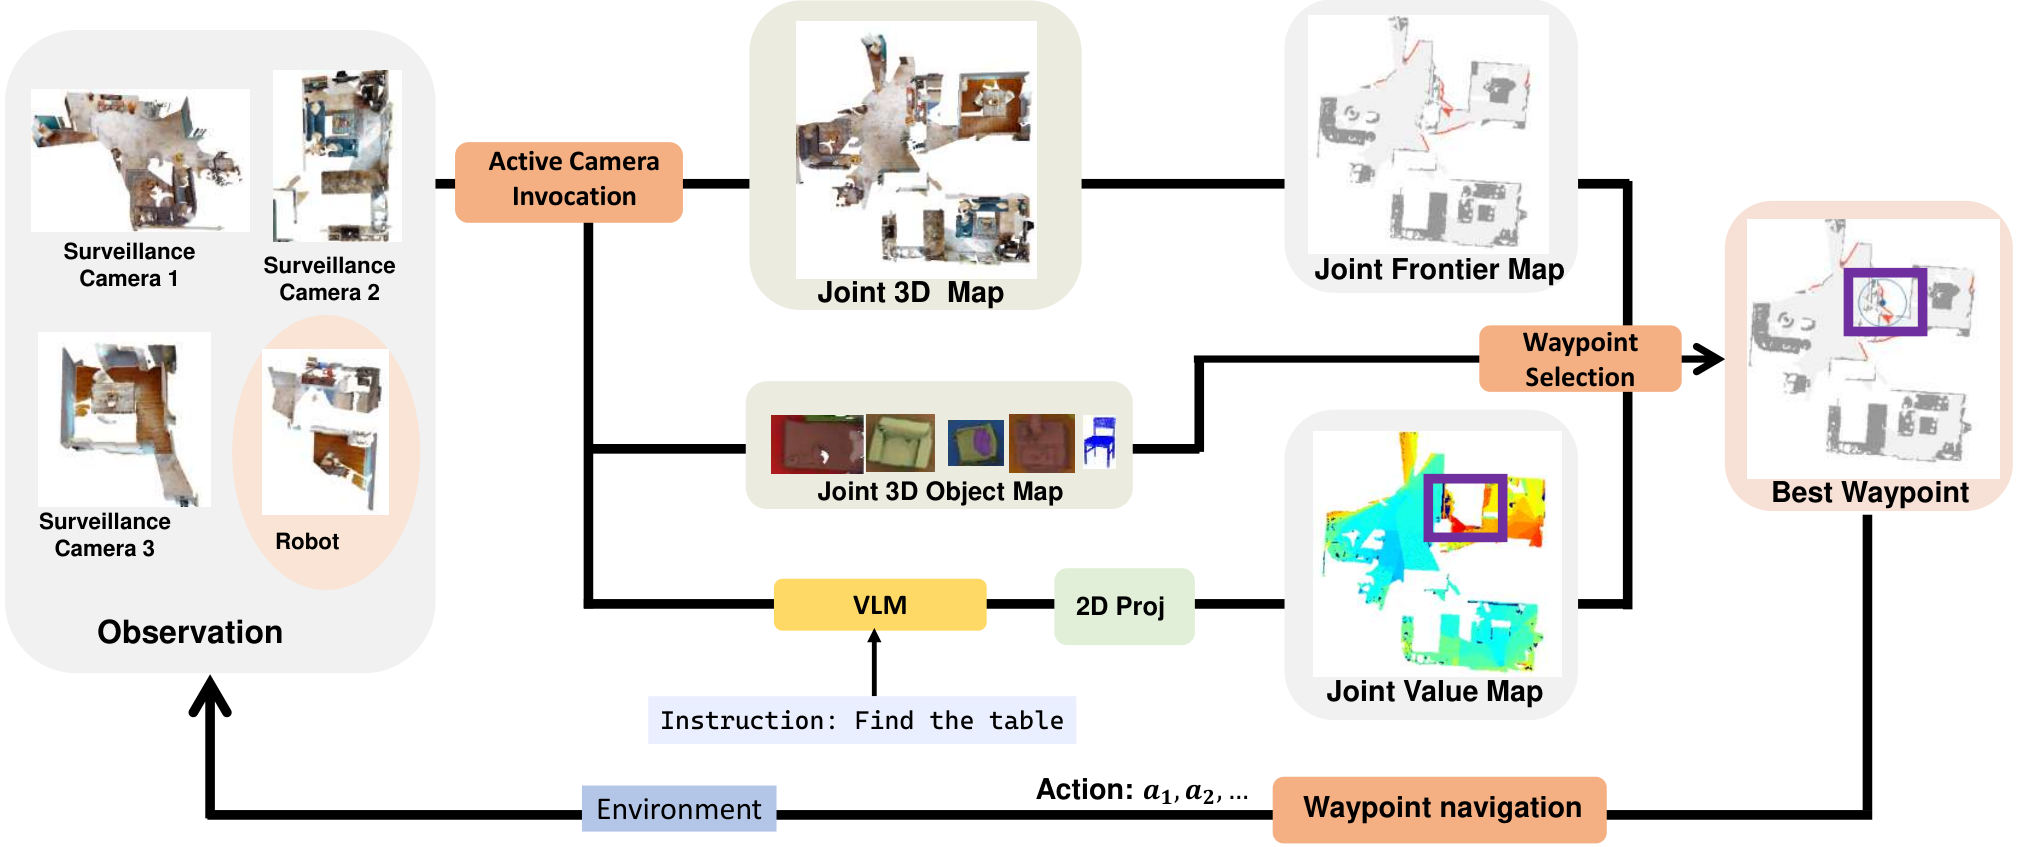
\includegraphics[width=\linewidth,height=28mm,keepaspectratio]{figures/p_surveilnav.png}\par{\fontsize{6.6}{8}\selectfont\color{muted}SurveilNav Fig.3：监控调用、共享地图与目标确认}\par\endgroup\vspace{1mm}

\noindent\begin{minipage}[t]{.323\linewidth}\vspace{0pt}\raggedright \ph{视角对齐}\quad 按楼层高度调用监控视角，将机器人和外部RGB-D都变换到共同坐标；形成共享点云、探索／障碍图及CLIP语义值图。\par\end{minipage}\hfill\begin{minipage}[t]{.323\linewidth}\vspace{0pt}\raggedright \ph{对象与规划}\quad Grounding DINO＋MobileSAM生成对象点云，按语义相似和几何IoU关联；多视角更新类别和置信，再选择对象或前沿航点。\par\end{minipage}\hfill\begin{minipage}[t]{.323\linewidth}\vspace{0pt}\raggedright \ph{实验发现}\quad 同FMM条件SR62.7→67.4，SPL26.1→34.5；提供GT深度和准确位姿，固定监控相机本身不发生移动。\par\end{minipage}
\takeaway{方法要点：外部相机先突破本体遮挡，机器人再用接近观察持续确认对象与通行信息。}
\note{SurveilNav基于HM3Dv2构建监控协作数据，按楼层面积布置相机并采多朝向观察。相机调用按同层支撑平面高度差阈值0.4米筛选。CLIP相关分数通过深度和相机位姿投到二维值图，监控和本体观察做融合；对象点云用几何IoU与语义特征联合关联，置信和类别随新增观察更新。实验中固定FMM比较最直接反映外部视角作用，SPL提高8.4点、SR提高4.7点。该工作说明异位观察能改善遮挡下搜索，为移动多机视角分配提供基础。}
\end{frame}
\gdef\slidesource{\href{https://arxiv.org/html/2609.03483v3}{[28] AGC-VLN} · §III–IV；Fig.2；Tables I、IV}
\begin{frame}[t,label=agcvln]{AGC-VLN：以标注俯视图连接空中定位与地面行驶}
\relax
\par\begingroup\centering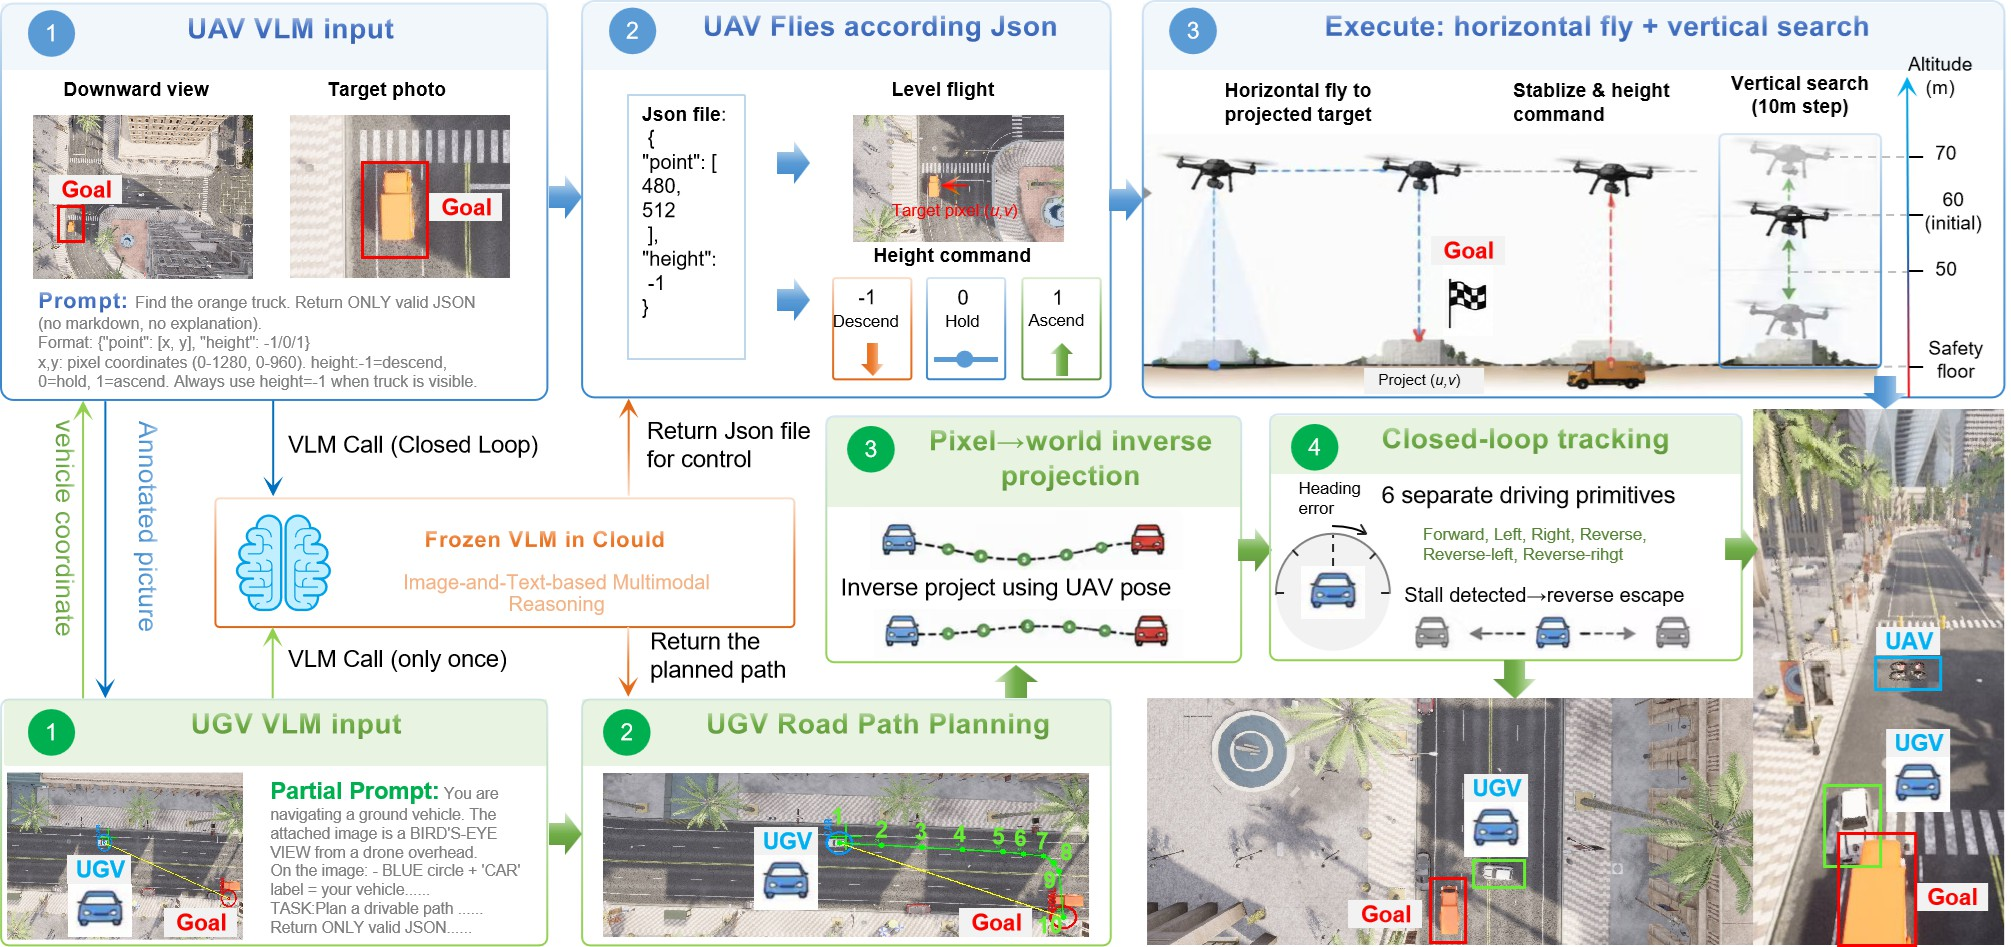
\includegraphics[width=\linewidth,height=26.5mm,keepaspectratio]{figures/p_agcvln.jpg}\par{\fontsize{6.6}{8}\selectfont\color{muted}AGC-VLN Fig.2：3D-SPF与共享鸟瞰路径规划}\par\endgroup\vspace{1mm}

\noindent\begin{minipage}[t]{.323\linewidth}\vspace{0pt}\raggedright \ph{空中模块}\quad 向下RGB送冻结VLM，返回目标像素与升降命令；平地射线转换目标位置，比例控制水平飞行并按10m步长调高度。\par\end{minipage}\hfill\begin{minipage}[t]{.323\linewidth}\vspace{0pt}\raggedright \ph{地面模块}\quad 共享图标注CAR、GOAL及距离，VLM生成10个道路像素点；以捕获位姿逆投影到世界坐标，六类驾驶原语闭环跟踪并解卡。\par\end{minipage}\hfill\begin{minipage}[t]{.323\linewidth}\vspace{0pt}\raggedright \ph{结果与条件}\quad 100回合、180s、5m范围：UGV75\%、UAV50\%、任一到达77\%。GOAL标记由回合目标坐标生成，重点检验跨视角路径接口。\par\end{minipage}
\takeaway{方法要点：共享俯视空间关系可直接服务道路规划，确定性的坐标变换将高层视觉决策接到各自控制器。}
\note{UAV与UGV读取同步位姿。空中3D-SPF利用VLM像素定位做自主接近，而发给UGV的共享图GOAL标记使用任务给定目标坐标。图中同时标UGV位置与距离，地面VLM得到相对全局上下文后规划10个沿道路航点；使用图像捕获时刻的UAV位姿逆投影，并转换AirSim NED与CARLA世界坐标。完整图注释的联合SR77，高于原图65；CAR+GOAL为70。任务联合成功定义为任意一方到达，系统优点在视角互补和清楚的几何接口，后续未知目标研究须增加自定位目标的共享机制。}
\end{frame}
\gdef\slidesource{\href{https://arxiv.org/html/2505.09108v1}{[11] Air-Ground}；\href{https://arxiv.org/html/2603.12908v2}{[25] GoalSwarm}；\href{https://arxiv.org/html/2603.20804v2}{[26] Co-VLN}；\href{https://arxiv.org/html/2606.25119v1}{[27] SurveilNav}；\href{https://arxiv.org/html/2609.03483v3}{[28] AGC-VLN} · 本报告架构比较}
\begin{frame}[t,label=external]{五类协作机制：共享什么、怎样影响行动}
\relax
{\fontsize{8.5}{10.8}\selectfont\rowcolors{2}{white}{zebra}
\begin{tabularx}{\linewidth}{@{}Y{0.65}Y{1.15}Y{1.2}@{}}\toprule\rowcolor{navy}\thd{工作} & \thd{共享的表示} & \thd{协作怎样产生作用}\\\midrule
Air-Ground & 可通行区域—对象图，语义类别请求 & 空中先验引导地面任务，近景验证并删改地图边\\
GoalSwarm & 占据图、语义均值／方差、预约前沿 & UCB探索与路程竞拍分配不同搜索方向\\
Co-VLN & 匹配节点后的拓扑与已有观察 & 扩充可达记忆，修正当前路线选择\\
SurveilNav & 外部＋本体对象点云及语义值图 & 异位视角突破遮挡，移动观察持续确认\\
AGC-VLN & 带位姿的CAR／GOAL俯视图 & 空中全局视角辅助地面道路规划\\
\bottomrule\end{tabularx}\par}
\takeaway{研究机会：把地图和历史共享进一步推进为“为共同问题主动取得互补观察”，按未决属性分配下一次感知动作。}
\note{五类协作分别在地图、效用、记忆、对象和图像层建立共享接口。它们已经提供区域分工、跨视角定位和历史复用。若共同任务由多个分散属性组成，例如建筑身份、标牌文字和入口通行，下一步要优化的是这些任务属性的联合可判定性，而不仅是搜索面积或目标坐标。下面方案由这些具体机制推导。}
\end{frame}
\gdef\slidesource{\href{https://arxiv.org/html/2502.18041v7}{[1] OpenFly}；\href{https://arxiv.org/html/2602.00708v2}{[7] USS-Nav}；\href{https://arxiv.org/html/2606.14772v1}{[12] ScoutVLA}；\href{https://arxiv.org/html/2609.39763v1}{[20] DiffWAM}；\href{https://arxiv.org/html/2610.25407v1}{[24] AeroDASH}；\href{https://arxiv.org/html/2603.12908v2}{[25] GoalSwarm}；\href{https://arxiv.org/html/2607.18060v3}{[29] RoboHarness（策略编排）} · 本报告综合分析}
\begin{frame}[t,label=synthesis]{研究判断：观测价值、动作先验与执行状态正在汇合}
\relax
{\fontsize{8.5}{10.8}\selectfont\rowcolors{2}{white}{zebra}
\begin{tabularx}{\linewidth}{@{}Y{0.75}Y{1.1}Y{1.15}@{}}\toprule\rowcolor{navy}\thd{技术演进} & \thd{文献支持} & \thd{对群体研究的具体启示}\\\midrule
历史压缩→空间记忆 & OpenFly、USS-Nav、RAVEN & 共享地图要保留对象、视角与定位精度\\
目标接近→问题取景 & AirHunt、ScoutVLA、ActiveFly、FlyCo & 观察任务应写清要获取的属性和视域条件\\
反应动作→预测运动 & ANWM、WorldFly、ForeFly、WorldVLN、Imagine、Diff & 未来用于候选提案和运动参考，反馈来自实际观察\\
单步输出→时序执行 & X-Fly、AeroDASH、两篇RoboHarness & 团队调度需考虑中断、接管与反馈\\
共享历史→主动分工 & Air-Ground、GoalSwarm、Co-VLN、Surveil、AGC & 根据共同任务缺失的信息选择队友与新视角\\
\bottomrule\end{tabularx}\par}
\takeaway{本报告的研究判断：群体层最值得建模的是“任务条件下的新观察价值”，单体层提供可替换的行动和执行能力。}
\note{此页是基于上述文献的综合判断。单体研究已经使观测选择、世界预测和连续执行变得可实现，多体研究也提供共享图与前沿分配。共同任务存在隐含的观察需求和成员能力差异时，可以把观察意图、视域、代价和时序作为统一动作单元，以条件边际价值驱动分工。后续研究不需要同时重训所有基础模型，而应先利用固定后端验证团队观察机制。}
\end{frame}
\section{拟开展研究}
\gdef\slidesource{拟研究方案：\href{https://arxiv.org/html/2606.14772v1}{[12] ScoutVLA}；\href{https://arxiv.org/html/2601.07558v1}{[14] FlyCo}；\href{https://arxiv.org/html/2601.12742v1}{[8] AirHunt}；\href{https://arxiv.org/html/2603.12908v2}{[25] GoalSwarm}；\href{https://arxiv.org/html/2603.20804v2}{[26] Co-VLN}}
\begin{frame}[t,label=proposal_problem]{研究方案：共同任务条件下的互补观察}
\relax
\lead{单体负责看和飞；群体负责决定谁去看、什么时候看、看到什么算数。}
\par\ph{共同任务}\quad 限定观察区内，找标牌为“实验室”且入口可通行的建筑，并让一名成员到达。相似外观让“到一个坐标”不足以判定完成。\par\vspace{1mm}
\par\ph{互补观察}\quad 高处视图缩候选区域；近景读标牌、关联身份；入口段用观测和规划/\allowbreak{}执行反馈验证通行。视域外保持未知，角色按状态和代价动态分。\par\vspace{1mm}
\par\ph{H1：观察分工}\quad 任务条件的互补观察，能否在同N、同单体、同预算下提高严格成功率，或降低达到同等质量的成本？\par\vspace{1mm}
\par\ph{H2：证据闭环}\quad 显式处理来源相关和反证撤销，能否在重放、近似视角、共同模型偏差下减少错误承诺和误停？\par\vspace{1mm}
\takeaway{研究对象：共同任务的属性缺口、互补视角选择，以及观察返回后的联合决策更新。}

\note{本报告提出三台同型无人机的首期仿真场景。共同任务需要同时判断建筑身份、标牌属性、入口局部通行性并让一名成员到达。任务变量和必要谓词明确后，将未知谓词转为候选观察；高视角适合缩小候选区域，近景适合读取细节，入口段观察结合几何和执行反馈验证局部通行。H1检验条件边际观察价值，H2检验相关证据和反证撤销的作用。}
\end{frame}
\gdef\slidesource{拟研究方案：\href{https://arxiv.org/html/2607.18060v3}{[29] RoboHarness（编排）}；\href{https://arxiv.org/html/2610.14018v2}{[30] RoboHarness（几何）}；\href{https://arxiv.org/html/2610.25407v1}{[24] AeroDASH}；\href{https://arxiv.org/html/2609.39763v1}{[20] DiffWAM}}
\begin{frame}[t,label=proposal_contract]{观察任务接口：目标、视域、时限与反馈}
\relax
\lead{VLA/\allowbreak{}WAM保留原生动作格式；harness包住模型和几何工具，对外提供可执行的观察服务。}
{\fontsize{8.0}{10.1}\selectfont
\rowcolors{2}{white}{zebra}
\begin{tabularx}{\linewidth}{@{}Y{0.48}Y{1.53}Y{0.99}@{}}\toprule
\rowcolor{navy}\thd{接口} & \thd{约定/\allowbreak{}返回} & \thd{作用}\\\midrule
propose & 对象/\allowbreak{}未决属性、候选视域；分辨率/\allowbreak{}能力、时长/\allowbreak{}风险/\allowbreak{}资源 & 比较候选，允许unknown/\allowbreak{}拒绝\\
execute & 坐标与时间锚、deadline、可打断点、局部回退、成功证据要求 & 处理推理滞后，接上计划\\
observe & 实测帧、捕获时间、位姿/\allowbreak{}不确定度、实例关联、来源链 & 把实测和预测分开\\
status & accepted/\allowbreak{}running/\allowbreak{}observed/\allowbreak{}failed/\allowbreak{}rejected、已执行前缀 & 撤销过期合同，及时重派\\
\bottomrule\end{tabularx}\par}

\noindent\begin{minipage}[t]{0.485\linewidth}\vspace{0pt}\raggedright \par\ph{三种后端各干什么}\quad VLA做局部取景；只有具备动作条件接口的WAM才评估候选后果；harness管工具和策略路由。\par\vspace{1mm}
\end{minipage}\hfill
\begin{minipage}[t]{0.485\linewidth}\vspace{0pt}\raggedright \par\ph{到无人机上}\quad 本地适配器负责运动可行性、轨迹接轨和超时检查；首期冻结单体，不把骨干升级的收益算给协作。\par\vspace{1mm}
\end{minipage}\par

\note{观察接口包含四类消息：propose提交未决属性、候选视域与预计成本；execute给坐标时间锚、中断点和局部回退；observe带回真实图像、位姿、时效、来源与属性支持；status报告接受、拒绝、执行中与结束。VLA用动作块、WAM用运动参考，harness负责工具调用与策略组织，但团队调度统一围绕观察任务工作。}
\end{frame}
\gdef\slidesource{拟研究方案：\href{https://arxiv.org/html/2603.12908v2}{[25] GoalSwarm}；\href{https://arxiv.org/html/2603.20804v2}{[26] Co-VLN}}
\begin{frame}[t,label=proposal_evidence]{任务证据状态：来源、时效与冲突更新}
\relax
\lead{从“大家都说是”改成“哪条实测支持哪项谓词、是否独立、什么时候失效”。}
{\fontsize{8.0}{10.1}\selectfont
\rowcolors{2}{white}{zebra}
\begin{tabularx}{\linewidth}{@{}Y{0.69}Y{1.29}Y{1.02}@{}}\toprule
\rowcolor{navy}\thd{观测关系} & \thd{风险} & \thd{处理与验证}\\\midrule
同帧多跳转发 & 一条测量被累成多票 & obs\_id/\allowbreak{}lineage去重；重放不增加独立证据\\
同帧新问题/\allowbreak{}新裁剪 & 语义解读被当成新传感 & 允许提取新属性，但保留同一物理来源\\
近似视角/\allowbreak{}同模型 & 遮挡和误检有共同原因 & 相关簇＋验证集校准，不直接独立相乘\\
新视角真实反证 & 旧承诺被锁死 & 版本化撤销，重开谓词，互补视角复查\\
\bottomrule\end{tabularx}\par}
\par\ph{最小状态}\quad 实例、任务谓词、支持/\allowbreak{}反证、原帧、捕获时间、位姿/\allowbreak{}可见范围、模型版本、来源链、承诺版本；没覆盖或过期就保持unknown。\par\vspace{1mm}
\par\ph{实现方式}\quad 先以支持—反证账本维护属性状态，加入观测ID去重、同源相关簇和反证撤销；再用验证集标定需要输出的置信度。\par\vspace{1mm}
\takeaway{H2要看错误承诺是否下降、撤销后恢复是否更快，而不只是日志更全。}

\note{状态将任务命题与来源关联。相同图像多跳转发只算一次采样；相似视角与共享模型形成相关簇；新的反证能够撤销既有属性承诺。预测候选和真实观测分别登记。动态状态设置有效期，负属性要求有限区域和足够覆盖。压力测试包括多跳重放、近似视角、共同误检和对象错关联。}
\end{frame}
\gdef\slidesource{拟研究方案}
\begin{frame}[t,label=proposal_value]{观察价值：共同任务风险的条件下降}
\relax
\lead{一条观察值不值得取，看它能不能改变任务判定，以及要花多少运动、计算和通信。}
\[F(A\mid E)=\mathbb E_{O_A\mid E}\left[\mathcal R(b_E,I)-\mathcal R(b_{E\cup O_A},I)\right]\]
\[A^*=\arg\max_{A\in\mathcal F}F(A\mid E)-\lambda_TC_T(A)-\lambda_EC_E(A)-\lambda_BC_B(A)\]
\par\ph{任务风险}\quad E是真实证据，I是共同指令；任务变量包括身份、属性、完成状态。R是当前证据下的最小决策损失；原型先用固定判定器的错误和严格成功事件做可测代理。\par\vspace{1mm}
\par\ph{估计路径}\quad 同一仿真状态分叉采集候选视图，比较固定判定器看前／看后的结果，训一个小型价值器。真值只做训练标签、评测和oracle上界，不进在线调度。\par\vspace{1mm}
\par\ph{边界与代价}\quad F是理论目标，概率解释依赖建模和校准；精确条件价值已含相关冗余，相似度罚项要单独消融。权重在验证集固定，另报时间／总能量／字节的Pareto。\par\vspace{1mm}
\takeaway{第一步先看：任务条件价值能不能比距离、前沿、覆盖更好地解释观察收益。}

\note{公式为拟研究的决策目标。用观察后共同任务风险的期望下降定义信息价值，再扣飞行、计算和通信代价。第一阶段用固定回答器的误差与严格任务成功作可测代理，利用同场景checkpoint分叉得到成对观察收益数据，按场景和对象隔离训练测试。学习的价值器在运行时只读团队当前状态和候选描述。}
\end{frame}
\gdef\slidesource{拟研究方案：\href{https://arxiv.org/html/2603.12908v2}{[25] GoalSwarm}；\href{https://arxiv.org/html/2512.21887v2}{[15] ANWM}；\href{https://arxiv.org/html/2609.33581v1}{[18] ForeFly}；\href{https://arxiv.org/html/2609.39763v1}{[20] DiffWAM}}
\begin{frame}[t,label=proposal_allocation]{观察分配：条件边际收益与动态重派}
\relax
{\fontsize{8.9}{11.0}\selectfont\lead{两个视角可能重复，也可能一起消歧；各机独立取最大值，往往不够。}
{\fontsize{8.0}{10.1}\selectfont
\rowcolors{2}{white}{zebra}
\begin{tabularx}{\linewidth}{@{}Y{0.48}Y{1.53}Y{0.99}@{}}\toprule
\rowcolor{navy}\thd{步骤} & \thd{原型方法} & \thd{关键对照}\\\midrule
生成 & 各机提视点、目标谓词、捕获时间和代价 & 同候选池，隔离候选质量\\
选择 & 条件于已选集合S；短期预约＋有限成对前瞻 & 独立最大值、距离／前沿、图竞拍\\
更新 & 用真实证据核来源／时效；撤销过期预约，重算缺口 & 固定分工、无撤销、周期重规划\\
\bottomrule\end{tabularx}\par}
\[\Delta_i(c\mid S,E)=F(S\cup\{(i,c)\}\mid E)-F(S\mid E)\]

\noindent\begin{minipage}[t]{0.485\linewidth}\vspace{0pt}\raggedright \par\ph{不假设次模}\quad 两个单独不充分的视角可能一起消歧；贪心／竞拍只是求解近似，不宣称1−1/\allowbreak{}e。成对前瞻要算计算开销并消融。\par\vspace{.3mm}
\end{minipage}\hfill
\begin{minipage}[t]{0.485\linewidth}\vspace{0pt}\raggedright \par\ph{WAM的角色}\quad 动作条件模型估候选后果；任务条件策略做单体执行器。预测要做失效检测，生成画面不是实测。首期冻结后端，WAM估值作为后续替换实验。\par\vspace{.3mm}
\end{minipage}\par
\takeaway{在队友已选观察的条件下重新估计增量，用已有竞拍或贪心算法完成可执行分配。}
}
\note{候选由各成员的地图、属性缺口和可达视域生成。团队先选择一个性价比高的观察，再在该观察已预约的条件下重算剩余候选边际收益，避免同时派往重复角度。反馈、超时或状态变化触发重派；对需要连续两个观察才能判定的任务加入成对前瞻。执行器依据当前动力学与安全约束接受或拒绝。}
\end{frame}
\gdef\slidesource{拟研究方案：\href{https://arxiv.org/html/2505.09108v1}{[11] Air-Ground}；\href{https://arxiv.org/html/2610.25407v1}{[24] AeroDASH}；\href{https://arxiv.org/html/2610.21450v1}{[23] X-Fly}；\href{https://arxiv.org/html/2609.03483v3}{[28] AGC-VLN}}
\begin{frame}[t,label=proposal_runtime]{运行闭环：任务派发、反馈与团队停止}
\relax
\lead{证据只有在有效时间内改变队友决策、并对应真实执行，才算团队作用。}
{\fontsize{8.0}{10.1}\selectfont
\rowcolors{2}{white}{zebra}
\begin{tabularx}{\linewidth}{@{}Y{0.48}Y{1.53}Y{0.99}@{}}\toprule
\rowcolor{navy}\thd{触发} & \thd{优先消息} & \thd{接收端怎么处理}\\\midrule
新候选/\allowbreak{}反证 & 实例/\allowbreak{}谓词/\allowbreak{}来源/\allowbreak{}时间/\allowbreak{}空间；必要时原裁剪 & 更新支持/\allowbreak{}反证，撤销失效目标\\
超期/\allowbreak{}执行失败 & 合同版本、已执行前缀、失败与回退 & 取消预约，重派缺失观察\\
证据冲突/\allowbreak{}复核 & 关联依据、待核命题、所需原帧 & 请求互补视角，不用多票代替核验\\
\bottomrule\end{tabularx}\par}
\par\ph{停止证书}\quad 同一身份；必要谓词有未过期的可追溯实测支持；指定执行反馈完成；没有未决关键反证。单体STOP只是事件，不算团队成功。\par\vspace{1mm}
\par\ph{时间怎么记}\quad 捕获／发送／接收／执行分开记，协议头和调度消息计字节；有界延迟下核承诺版本，断链按本地合同回退。\par\vspace{1mm}
\par\ph{指标分开}\quad SR\_union、指定成员到达、SR\_task分报；另报误停、漏停、错误承诺、证据年龄和无效继续观察的成本。\par\vspace{1mm}
\takeaway{通信和停止规则是H1/H2落地与审计的支撑；首期不同时承诺协议创新。}

\note{通信分为属性更新、预约和执行状态、冲突复核三类。团队结束需要目标身份一致、必要属性有有效真实观察支持、指定执行反馈完成以及关键冲突已处理。日志记录观察捕获、消息到达、计划生效和执行完成四个时间，以分析通信和推理延迟。}
\end{frame}
\gdef\slidesource{拟研究方案：\href{https://arxiv.org/html/2502.18041v7}{[1] OpenFly}；\href{https://arxiv.org/html/2410.07087v2}{[2] TravelUAV}；\href{https://arxiv.org/html/2606.14772v1}{[12] ScoutVLA}；\href{https://arxiv.org/html/2603.12908v2}{[25] GoalSwarm}；\href{https://arxiv.org/html/2603.20804v2}{[26] Co-VLN}}
\begin{frame}[t,label=proposal_experiment]{实验设计：固定团队与总资源的机制比较}
\relax
\lead{首期只动团队观察决策和证据处理；同N、同后端，才能把增益归到团队层。}
{\fontsize{8.0}{10.1}\selectfont
\rowcolors{2}{white}{zebra}
\begin{tabularx}{\linewidth}{@{}Y{0.5}Y{1.5}@{}}\toprule
\rowcolor{navy}\thd{设计} & \thd{具体方案}\\\midrule
任务A：目标消歧 & 相似建筑、背面属性、错误初始grounding；局部通行限定ROI/\allowbreak{}覆盖\\
任务B：分布式EQA & 跨视角各含部分属性，固定回答器；记录前后答案/\allowbreak{}依据\\
数据与划分 & 复用OpenFly/\allowbreak{}TravelUAV场景工具链，新建多体同步任务/\allowbreak{}划分；GT只做标签/\allowbreak{}评估\\
同团队基线 & 独立；区域/\allowbreak{}前沿；仅共享历史；GoalSwarm式图竞拍；条件价值；完整闭环\\
\bottomrule\end{tabularx}\par}
\par\ph{A：总资源等额}\quad 固定N、总图像／调用、总飞行或能量、字节和最大时限；GPU秒与协议开销同计。\par\vspace{1mm}
\par\ph{B：固定截止时间}\quad 固定团队墙钟，另报总能量／算力／字节，看并行部署收益；与A分开。N=1是强单体参考，不是唯一对照。\par\vspace{1mm}
\takeaway{先在同一个N和预算下证明机制，再扩规模与异构。}

\note{固定三台同型UAV与单体策略，比较独立探索、区域前沿分工、仅共享历史、GoalSwarm式地图竞拍、条件观察价值以及完整证据闭环。任务A为相似目标消歧，任务B为分布式问答。总资源等额实验固定总图像、飞行、计算和通信预算；固定截止时间实验另测并行收益。真实地图和目标属性仅用于离线标签与评价。}
\end{frame}
\gdef\slidesource{拟研究方案}
\begin{frame}[t,label=proposal_eval]{评价设计：任务完成、信息贡献与执行成本}
\relax
\lead{除了最终SR，还要分清是看得更好、证据更可靠，还是单纯多花了资源。}
{\fontsize{8.0}{10.1}\selectfont
\rowcolors{2}{white}{zebra}
\begin{tabularx}{\linewidth}{@{}Y{0.48}Y{1.53}Y{0.99}@{}}\toprule
\rowcolor{navy}\thd{层级} & \thd{主指标} & \thd{控制什么}\\\midrule
任务 & SR\_task、身份/\allowbreak{}属性/\allowbreak{}到达分解、误停/\allowbreak{}漏停 & 并集到达不能冒充共同任务\\
观察 & 固定回答器增益、新属性证据/\allowbreak{}调用、必要视角覆盖 & 不换回答器，不无限采样\\
证据 & 误承诺、重复计证、反证恢复率/\allowbreak{}时长 & 不用未校准多票当置信\\
资源 & 墙钟、总能量/\allowbreak{}路程、GPU秒、bytes、负载 & 不用更多硬件冒充协同效率\\
执行 & 超期/\allowbreak{}拒绝/\allowbreak{}接管失败、碰撞、扰动曲线 & 不只统计成功回合的耗时\\
\bottomrule\end{tabularx}\par}

\noindent\begin{minipage}[t]{0.3233333333333333\linewidth}\vspace{0pt}\raggedright \par\ph{H1归因}\quad 同候选池：距离／覆盖\ensuremath{\to}独立价值\ensuremath{\to}条件价值\ensuremath{\to}成对前瞻；固定证据模块和计算预算。\par\vspace{1mm}
\end{minipage}\hfill
\begin{minipage}[t]{0.3233333333333333\linewidth}\vspace{0pt}\raggedright \par\ph{H2归因}\quad 固定分配器：无来源\ensuremath{\to}仅ID\ensuremath{\to}相关簇\ensuremath{\to}反证撤销；分别注入多跳重放、近似视角、共同误检。Brier/\allowbreak{}ECE只用于校准过的概率配置。\par\vspace{1mm}
\end{minipage}\hfill
\begin{minipage}[t]{0.3233333333333333\linewidth}\vspace{0pt}\raggedright \par\ph{统计}\quad 预定主指标、配对任务、多随机种子；按任务／场景依赖给置信区间，保留所有失败和超时；区分训练重复与只评估重复。\par\vspace{1mm}
\end{minipage}\par

\note{分别消融观察价值和证据处理。H1在相同候选与证据模块下比较距离、覆盖、独立价值、条件价值及成对前瞻；H2固定分配器，比较无来源、ID去重、相关簇与反证撤销。报告严格任务成功率、固定回答器增益、误停、错误属性承诺、恢复时间及全部资源，采用配对任务和多随机种子。}
\end{frame}
\gdef\slidesource{拟研究方案}
\begin{frame}[t,label=proposal_close]{拟开展研究：群体任务条件主动感知}
\relax
\lead{VLA/\allowbreak{}WAM给单体行动能力，harness把工具、状态和反馈接起来；群体研究的是互补观察和证据闭环。}
{\fontsize{8.0}{10.1}\selectfont
\rowcolors{2}{white}{zebra}
\begin{tabularx}{\linewidth}{@{}Y{0.69}Y{1.29}Y{1.02}@{}}\toprule
\rowcolor{navy}\thd{核心假设} & \thd{支持证据} & \thd{什么情况下不成立}\\\midrule
H1：互补观察 & 同N同预算优于覆盖/\allowbreak{}独立估值，固定回答器增益提高 & 只靠加模型/\allowbreak{}观测/\allowbreak{}算力，条件化没作用\\
H2：相关证据与撤销 & 重放/\allowbreak{}共同误检下误承诺更少，反证恢复更快 & 只多了日志，误停不降或任务质量明显下降\\
\bottomrule\end{tabularx}\par}
\par\ph{阶段1：因果证据}\quad 冻结单体，中心式审计调度；先建任务、候选和同预算强基线。\par\vspace{.5mm}
\par\ph{阶段2：学习与鲁棒}\quad 配对分叉数据训小型价值器；加入遮挡、关联错误、通信／位姿扰动，测泛化和失效。\par\vspace{.5mm}
\par\ph{阶段3：后端与真机}\quad 替换VLA/\allowbreak{}WAM/\allowbreak{}harness接口比较成本；再做两机真实场景、规模和异构。WAM估值和端到端多体学习放在后面。\par\vspace{.5mm}
\takeaway{预期成果：以任务属性为单位的群体主动感知方法、可复用观察接口，以及预算受限的协作评价基准。}

\end{frame}
\section{参考文献}
\gdef\slidesource{\href{https://arxiv.org/html/2502.18041v7}{[1] OpenFly}；\href{https://arxiv.org/html/2410.07087v2}{[2] TravelUAV / OpenUAV}；\href{https://arxiv.org/html/2505.15725v2}{[3] UAV-Flow}；\href{https://arxiv.org/html/2506.02896v3}{[4] FlySearch}；\href{https://arxiv.org/html/2603.14363v1}{[5] AerialVLA}}
\begin{frame}[t,label=refs1]{参考文献 1/6：固定版本与完整题名}
\relax
{\fontsize{8.3}{10.6}\selectfont
\par\textcolor{teal}{\textbf{[1] OpenFly} Yunpeng Gao et al., 2025}\quad OpenFly: A Comprehensive Platform for Aerial Vision-Language Navigation.\par\href{https://arxiv.org/html/2502.18041v7}{arXiv:2502.18041v7}\par\vspace{1.8mm}
\par\textcolor{teal}{\textbf{[2] TravelUAV / OpenUAV} Xiangyu Wang et al., 2024}\quad Towards Realistic UAV Vision-Language Navigation: Platform, Benchmark, and Methodology.\par\href{https://arxiv.org/html/2410.07087v2}{arXiv:2410.07087v2}\par\vspace{1.8mm}
\par\textcolor{teal}{\textbf{[3] UAV-Flow} Xiangyu Wang et al., 2025}\quad UAV-Flow Colosseo: A Real-World Benchmark for Flying-on-a-Word UAV Imitation Learning.\par\href{https://arxiv.org/html/2505.15725v2}{arXiv:2505.15725v2}\par\vspace{1.8mm}
\par\textcolor{teal}{\textbf{[4] FlySearch} Adam Pardyl et al., 2025}\quad FlySearch: Exploring how vision-language models explore.\par\href{https://arxiv.org/html/2506.02896v3}{arXiv:2506.02896v3}\par\vspace{1.8mm}
\par\textcolor{teal}{\textbf{[5] AerialVLA} Peng Xu et al., 2026}\quad AerialVLA: A Vision-Language-Action Model for UAV Navigation via Minimalist End-to-End Control.\par\href{https://arxiv.org/html/2603.14363v1}{arXiv:2603.14363v1}\par\vspace{1.8mm}
}
\end{frame}
\gdef\slidesource{\href{https://arxiv.org/html/2512.15258v2}{[6] VLA-AN}；\href{https://arxiv.org/html/2602.00708v2}{[7] USS-Nav}；\href{https://arxiv.org/html/2601.12742v1}{[8] AirHunt}；\href{https://arxiv.org/html/2602.00551v1}{[9] APEX}；\href{https://arxiv.org/html/2509.23563v1}{[10] RAVEN}}
\begin{frame}[t,label=refs2]{参考文献 2/6：固定版本与完整题名}
\relax
{\fontsize{8.3}{10.6}\selectfont
\par\textcolor{teal}{\textbf{[6] VLA-AN} Yuze Wu et al., 2025}\quad VLA-AN: An Efficient and Onboard Vision-Language-Action Framework for Aerial Navigation in Complex Environments.\par\href{https://arxiv.org/html/2512.15258v2}{arXiv:2512.15258v2}\par\vspace{1.8mm}
\par\textcolor{teal}{\textbf{[7] USS-Nav} Weiqi Gai et al., 2026}\quad USS-Nav: Unified Spatio-Semantic Scene Graph for Lightweight UAV Zero-Shot Object Navigation.\par\href{https://arxiv.org/html/2602.00708v2}{arXiv:2602.00708v2}\par\vspace{1.8mm}
\par\textcolor{teal}{\textbf{[8] AirHunt} Xuecheng Chen et al., 2026}\quad AirHunt: Bridging VLM Semantics and Continuous Planning for Efficient Aerial Object Navigation.\par\href{https://arxiv.org/html/2601.12742v1}{arXiv:2601.12742v1}\par\vspace{1.8mm}
\par\textcolor{teal}{\textbf{[9] APEX} Daoxuan Zhang et al., 2026}\quad APEX: A Decoupled Memory-based Explorer for Asynchronous Aerial Object Goal Navigation.\par\href{https://arxiv.org/html/2602.00551v1}{arXiv:2602.00551v1}\par\vspace{1.8mm}
\par\textcolor{teal}{\textbf{[10] RAVEN} Seungchan Kim et al., 2025}\quad RAVEN: Resilient Aerial Navigation via Open-Set Semantic Memory and Behavior Adaptation.\par\href{https://arxiv.org/html/2509.23563v1}{arXiv:2509.23563v1}\par\vspace{1.8mm}
}
\end{frame}
\gdef\slidesource{\href{https://arxiv.org/html/2505.09108v1}{[11] Air-Ground}；\href{https://arxiv.org/html/2606.14772v1}{[12] ScoutVLA}；\href{https://arxiv.org/html/2607.10180v2}{[13] ActiveFly-Bench}；\href{https://arxiv.org/html/2601.07558v1}{[14] FlyCo}；\href{https://arxiv.org/html/2512.21887v2}{[15] ANWM}}
\begin{frame}[t,label=refs3]{参考文献 3/6：固定版本与完整题名}
\relax
{\fontsize{8.3}{10.6}\selectfont
\par\textcolor{teal}{\textbf{[11] Air-Ground} Fernando Cladera et al., 2025}\quad Air-Ground Collaboration for Language-Specified Missions in Unknown Environments.\par\href{https://arxiv.org/html/2505.09108v1}{arXiv:2505.09108v1}\par\vspace{1.8mm}
\par\textcolor{teal}{\textbf{[12] ScoutVLA} Wenhao Lu et al., 2026}\quad ScoutVLA: UAV-Centric Active Perception via a Dual-Expert VLA Model for Open-World Embodied Question Answering.\par\href{https://arxiv.org/html/2606.14772v1}{arXiv:2606.14772v1}\par\vspace{1.8mm}
\par\textcolor{teal}{\textbf{[13] ActiveFly-Bench} Weichen Zhang et al., 2026}\quad ActiveFly-Bench: Aligning Embodied Question Answering with Vision-Language-Action for Aerial Embodied Perception.\par\href{https://arxiv.org/html/2607.10180v2}{arXiv:2607.10180v2}\par\vspace{1.8mm}
\par\textcolor{teal}{\textbf{[14] FlyCo} Chen Feng et al., 2026}\quad FlyCo: Foundation Model-Empowered Drones for Autonomous 3D Structure Scanning in Open-World Environments.\par\href{https://arxiv.org/html/2601.07558v1}{arXiv:2601.07558v1}\par\vspace{1.8mm}
\par\textcolor{teal}{\textbf{[15] ANWM} Weichen Zhang et al., 2025}\quad Aerial World Model for Long-horizon Visual Generation and Navigation in 3D Space.\par\href{https://arxiv.org/html/2512.21887v2}{arXiv:2512.21887v2}\par\vspace{1.8mm}
}
\end{frame}
\gdef\slidesource{\href{https://arxiv.org/html/2605.15964v1}{[16] WorldVLN}；\href{https://arxiv.org/html/2606.06147v1}{[17] WorldFly}；\href{https://arxiv.org/html/2609.33581v1}{[18] ForeFly}；\href{https://arxiv.org/html/2606.01205v2}{[19] ImagineUAV}；\href{https://arxiv.org/html/2609.39763v1}{[20] DiffWAM}}
\begin{frame}[t,label=refs4]{参考文献 4/6：固定版本与完整题名}
\relax
{\fontsize{8.3}{10.6}\selectfont
\par\textcolor{teal}{\textbf{[16] WorldVLN} Baining Zhao et al., 2026}\quad WorldVLN: Autoregressive World Action Model for Aerial Vision-Language Navigation.\par\href{https://arxiv.org/html/2605.15964v1}{arXiv:2605.15964v1}\par\vspace{1.8mm}
\par\textcolor{teal}{\textbf{[17] WorldFly} Shengtao Zheng et al., 2026}\quad WorldFly: A World-Model-Based Vision-Language-Action Model for UAV Navigation.\par\href{https://arxiv.org/html/2606.06147v1}{arXiv:2606.06147v1}\par\vspace{1.8mm}
\par\textcolor{teal}{\textbf{[18] ForeFly} Kunhui Wang et al., 2026}\quad ForeFly: A Dual-Horizon World Action Model for Aerial Vision-Language Navigation.\par\href{https://arxiv.org/html/2609.33581v1}{arXiv:2609.33581v1}\par\vspace{1.8mm}
\par\textcolor{teal}{\textbf{[19] ImagineUAV} Xuchen Liu et al., 2026}\quad ImagineUAV: Aerial Vision-Language Navigation via World-Action Modeling and Kinodynamic Planning.\par\href{https://arxiv.org/html/2606.01205v2}{arXiv:2606.01205v2}\par\vspace{1.8mm}
\par\textcolor{teal}{\textbf{[20] DiffWAM} Mo Zhu et al., 2026}\quad DiffWAM: A Fast and Efficient Navigation World Action Model.\par\href{https://arxiv.org/html/2609.39763v1}{arXiv:2609.39763v1}\par\vspace{1.8mm}
}
\end{frame}
\gdef\slidesource{\href{https://arxiv.org/html/2608.09467v3}{[21] RefineFly}；\href{https://arxiv.org/html/2606.02313v1}{[22] EG-GRPO}；\href{https://arxiv.org/html/2610.21450v1}{[23] X-Fly}；\href{https://arxiv.org/html/2610.25407v1}{[24] AeroDASH}；\href{https://arxiv.org/html/2603.12908v2}{[25] GoalSwarm}}
\begin{frame}[t,label=refs5]{参考文献 5/6：固定版本与完整题名}
\relax
{\fontsize{8.3}{10.6}\selectfont
\par\textcolor{teal}{\textbf{[21] RefineFly} Boxiong Wang et al., 2026}\quad RefineFly: Failure-Aware Post-Training for Aerial Vision-Language Navigation.\par\href{https://arxiv.org/html/2608.09467v3}{arXiv:2608.09467v3}\par\vspace{1.8mm}
\par\textcolor{teal}{\textbf{[22] EG-GRPO} Tianyang Chen et al., 2026}\quad Towards Precise Intent-Aligned VLA Aerial Navigation via Expert-Guided GRPO.\par\href{https://arxiv.org/html/2606.02313v1}{arXiv:2606.02313v1}\par\vspace{1.8mm}
\par\textcolor{teal}{\textbf{[23] X-Fly} Ruibin Ju et al., 2026}\quad X-Fly: Learning to Reach and Stop in Full-Chunk Aerial Vision-Language Navigation.\par\href{https://arxiv.org/html/2610.21450v1}{arXiv:2610.21450v1}\par\vspace{1.8mm}
\par\textcolor{teal}{\textbf{[24] AeroDASH} Zhe Liu et al., 2026}\quad AeroDASH: Asynchronous Vision-Language-Action Control for Continuous UAV Flight.\par\href{https://arxiv.org/html/2610.25407v1}{arXiv:2610.25407v1}\par\vspace{1.8mm}
\par\textcolor{teal}{\textbf{[25] GoalSwarm} MoniJesu James et al., 2026}\quad GoalSwarm: Multi-UAV Semantic Coordination for Open-Vocabulary Object Navigation.\par\href{https://arxiv.org/html/2603.12908v2}{arXiv:2603.12908v2}\par\vspace{1.8mm}
}
\end{frame}
\gdef\slidesource{\href{https://arxiv.org/html/2603.20804v2}{[26] Co-VLN}；\href{https://arxiv.org/html/2606.25119v1}{[27] SurveilNav}；\href{https://arxiv.org/html/2609.03483v3}{[28] AGC-VLN}；\href{https://arxiv.org/html/2607.18060v3}{[29] RoboHarness（策略编排）}；\href{https://arxiv.org/html/2610.14018v2}{[30] RoboHarness（几何工具）}}
\begin{frame}[t,label=refs6]{参考文献 6/6：固定版本与完整题名}
\relax
{\fontsize{8.3}{10.6}\selectfont
\par\textcolor{teal}{\textbf{[26] Co-VLN} Qunchao Jin et al., 2026}\quad Does Peer Observation Help? Vision-Sharing Collaboration for Vision-Language Navigation.\par\href{https://arxiv.org/html/2603.20804v2}{arXiv:2603.20804v2}\par\vspace{1.8mm}
\par\textcolor{teal}{\textbf{[27] SurveilNav} Ming-Ming Yu et al., 2026}\quad SurveilNav: Collaborative Object Goal Navigation with Robot and Surveillance System.\par\href{https://arxiv.org/html/2606.25119v1}{arXiv:2606.25119v1}\par\vspace{1.8mm}
\par\textcolor{teal}{\textbf{[28] AGC-VLN} Shuning Zhang et al., 2026}\quad Air-Ground Collaborative Vision-and-Language Navigation via Shared Bird’s-Eye Maps.\par\href{https://arxiv.org/html/2609.03483v3}{arXiv:2609.03483v3}\par\vspace{1.8mm}
\par\textcolor{teal}{\textbf{[29] RoboHarness（策略编排）} Jinbang Huang et al., 2026}\quad RoboHarness: Memory-Driven Orchestration of Heterogeneous Robot Policies for Long-Horizon Planning.\par\href{https://arxiv.org/html/2607.18060v3}{arXiv:2607.18060v3}\par\vspace{1.8mm}
\par\textcolor{teal}{\textbf{[30] RoboHarness（几何工具）} Bince Qu et al., 2026}\quad RoboHarness: A Simple Harness Outperforms VLA and World Action Models.\par\href{https://arxiv.org/html/2610.14018v2}{arXiv:2610.14018v2}\par\vspace{1.8mm}
}
\end{frame}
\end{document}
